\documentclass[12pt,oneside]{book}

%%%%%%%%%%%%%%%%%%%%%%%%%%%%%%%%%%%%%%%%%%%%%%%%%%%%%%%%%%%%%%%%%%%%%%%%%%%%%%%%%%%%%%%%%%%%%%%%%%%
%                                                                                                 %
% The mathematical style of these documents follows                                               %
%                                                                                                 %
% A. Thompson and B.N. Taylor. The NIST Guide for the Use of the International System of Units.   %
%    NIST Special Publication 881, 2008.                                                          %
%                                                                                                 %
% http://www.nist.gov/pml/pubs/sp811/index.cfm                                                    %
%                                                                                                 %
%%%%%%%%%%%%%%%%%%%%%%%%%%%%%%%%%%%%%%%%%%%%%%%%%%%%%%%%%%%%%%%%%%%%%%%%%%%%%%%%%%%%%%%%%%%%%%%%%%%

% $Date: 2013-11-26 10:43:59 -0500 (Tue, 26 Nov 2013) $
% $Revision: 17538 $
% $Author: gforney $

%%%%%%%%%%%%%%%%%%%%%%%%%%%%%%%%%%%%%%%%%%%%%%%%%%%%%%%%%%%%%%%%%%%%%%%%%%%%%%%%%%%%%%%%%%%%%%%%%%%
%                                                                                                 %
% The mathematical style of these documents follows                                               %
%                                                                                                 %
% A. Thompson and B.N. Taylor. The NIST Guide for the Use of the International System of Units.   %
%    NIST Special Publication 881, 2008.                                                          %
%                                                                                                 %
% http://www.nist.gov/pml/pubs/sp811/index.cfm                                                    %
%                                                                                                 %
%%%%%%%%%%%%%%%%%%%%%%%%%%%%%%%%%%%%%%%%%%%%%%%%%%%%%%%%%%%%%%%%%%%%%%%%%%%%%%%%%%%%%%%%%%%%%%%%%%%

% Packages which force the use of better TeX coding
% Mostly from http://tex.stackexchange.com/q/19264
%%\RequirePackage[l2tabu, orthodox]{nag}
%%\usepackage{fixltx2e}
%\usepackage{isomath} % Disabled for the moment because it changes the syntax for bold and roman Greek math symbols
%%\usepackage[all,warning]{onlyamsmath}
%\usepackage{strict} % Commented out for now because it is uncommon. A copy of style.sty is in Manuals/LaTeX_Style_Files/.

\usepackage{times,mathptmx}
\usepackage[pdftex]{graphicx}
\usepackage{tabularx,ragged2e,booktabs,caption}
\usepackage{multirow}
\usepackage{pdfsync}
\usepackage{tikz}
\usepackage{pgfplots}
%\pgfplotsset{compat=1.7}
\usepackage{tocloft}
\usepackage{color}
\usepackage{amsmath}
\definecolor{linknavy}{rgb}{0,0,0.50196}
\definecolor{linkred}{rgb}{1,0,0}
\definecolor{linkblue}{rgb}{0,0,1}
\usepackage{float}
\usepackage{caption}
\usepackage{graphpap}
\usepackage{rotating}
\usepackage{graphicx}
\usepackage{geometry}
\usepackage{relsize}
\usepackage{longtable}
\usepackage{lscape}
\usepackage{amssymb}
\usepackage{makeidx} % Create index at end of document
\usepackage[nottoc,notlof,notlot]{tocbibind} % Put the bibliography and index in the ToC
\usepackage{lastpage} % Automatic last page number reference.
\usepackage[T1]{fontenc}
\usepackage{enumerate}
\usepackage{upquote}
\usepackage{moreverb}
\usepackage{xfrac}
\usepackage{cite}

\newcommand{\nopart}{\expandafter\def\csname Parent-1\endcsname{}} % To fix table of contents in pdf.
\newcommand{\ct}{\tt\small} % eventually will be deprecated due to http://www.tex.ac.uk/cgi-bin/texfaq2html?label=2letterfontcmd
\newcommand{\textct}[1]{\texttt{\small #1}}

\usepackage{tocstyle} % Fix table of contents sections from overlapping section titles
\usetocstyle{standard}
\usepackage{siunitx}
\sisetup{
    detect-all = true,
    input-decimal-markers = {.},
    input-ignore = {,},
    inter-unit-product = \ensuremath{{}\cdot{}},
    multi-part-units = repeat,
    number-unit-product = \text{~},
    per-mode = fraction,
    separate-uncertainty = true,
}

\usepackage{listings}
\usepackage{textcomp}
\definecolor{lbcolor}{rgb}{0.96,0.96,0.96}
\lstset{
    %backgroundcolor=\color{lbcolor},
    tabsize=4,
    rulecolor=,
    language=Fortran,
        basicstyle=\footnotesize\ttfamily,
        upquote=true,
        aboveskip={\baselineskip},
        belowskip={\baselineskip},
        columns=fixed,
        extendedchars=true,
        breaklines=true,
        breakatwhitespace=true,
        frame=none,
        showtabs=false,
        showspaces=false,
        showstringspaces=false,
        identifierstyle=\ttfamily,
        keywordstyle=\color[rgb]{0,0,0},
        commentstyle=\color[rgb]{0,0,0},
        stringstyle=\color[rgb]{0,0,0},
}

\usepackage[pdftex,
        colorlinks=true,
        urlcolor=linkblue,     % \href{...}{...} external (URL)
        citecolor=linkred,     % citation number colors
        linkcolor=linknavy,    % \ref{...} and \pageref{...}
        pdfproducer={pdflatex},
        pdfpagemode=UseNone,
        bookmarksopen=true,
        plainpages=false,
        verbose]{hyperref}

% The Following commented code makes the ``Draft'' watermark on each page.
%\usepackage{eso-pic}
%\usepackage{type1cm}
%\makeatletter
%   \AddToShipoutPicture{
%     \setlength{\@tempdimb}{.5\paperwidth}
%     \setlength{\@tempdimc}{.5\paperheight}
%     \setlength{\unitlength}{1pt}
%     \put(\strip@pt\@tempdimb,\strip@pt\@tempdimc){
%     \makebox(0,0){\rotatebox{45}{\textcolor[gray]{0.75}{\fontsize{8cm}\selectfont{RC6}}}}}
% }
%\makeatother

\setlength{\textwidth}{6.5in}
\setlength{\textheight}{9.0in}
\setlength{\topmargin}{0.in}
\setlength{\headheight}{0.pt}
\setlength{\headsep}{0.in}
\setlength{\parindent}{0.25in}
\setlength{\oddsidemargin}{0.0in}
\setlength{\evensidemargin}{0.0in}
\setlength{\leftmargini}{\parindent} % Controls the indenting of the "bullets" in a list
\setlength{\cftsecnumwidth}{0.45in}
\setlength{\cftsubsecnumwidth}{0.5in}
\setlength{\cftfignumwidth}{0.45in}
\setlength{\cfttabnumwidth}{0.45in}

\newcommand{\titlesigs}
{
\small
\flushright{U.S. Department of Commerce \\
{\em Penny Pritzker, Secretary} \\
\hspace{1in} \\
National Institute of Standards and Technology \\
{\em Willie May, Under Secretary of Commerce for Standards and Technology and Acting Director} }
}

% commands to use for "official" cover and title pages
% see smokeview verification guide to see how they are used

\newcommand{\headerA}[1]{
\flushright{
\fontsize{20}{24}\selectfont
\bf{NIST Special Publication #1}}
}

\newcommand{\headerB}[1]{
\flushright{
\fontsize{28}{33.6}\selectfont
\bf{#1}
}
}

\newcommand{\headerC}[1]{
\vspace{.5in}
\flushright{\fontsize{14}{16.8}\selectfont
#1}
}

\frenchspacing

\newcommand{\dod}[2]{\frac{\partial #1}{\partial #2}}
\newcommand{\DoD}[2]{\frac{\mathrm{D} #1}{\mathrm{D} #2}}
\newcommand{\dsods}[2]{\frac{\partial^2 #1}{\partial #2^2}}
\renewcommand{\d}{\,\mathrm{d}}
\newcommand{\dx}{\delta x}
\newcommand{\dy}{\delta y}
\newcommand{\dz}{\delta z}
\newcommand{\degF}{$^\circ$F}
\newcommand{\degC}{$^\circ$C}
\newcommand{\x}{x}
\newcommand{\y}{y}
\newcommand{\z}{z}
\newcommand{\dt}{\delta t}
\newcommand{\dn}{\delta n}
\newcommand{\cH}{H}
\newcommand{\hu}{u}
\newcommand{\hv}{v}
\newcommand{\hw}{w}
\newcommand{\la}{\lambda}
\newcommand{\bO}{{\Omega}}
\newcommand{\bo}{{\mathbf{\omega}}}
\newcommand{\btau}{\mathbf{\tau}}
\newcommand{\bdelta}{{\mathbf{\delta}}}
\newcommand{\sumyw}{\sum (Y_\alpha/W_\alpha)}
\newcommand{\oW}{\overline{W}}
\newcommand{\om}{\ensuremath{\omega}}
\newcommand{\omx}{\omega_x}
\newcommand{\omy}{\omega_y}
\newcommand{\omz}{\omega_z}
\newcommand{\erf}{\hbox{erf}}
\newcommand{\erfc}{\hbox{erfc}}
\newcommand{\bF}{{\mathbf{F}}}
\newcommand{\bG}{{\mathbf{G}}}
\newcommand{\bof}{{\mathbf{f}}}
\newcommand{\bq}{{\mathbf{q}}}
\newcommand{\br}{{\mathbf{r}}}
\newcommand{\bu}{{\mathbf{u}}}
\newcommand{\bx}{{\mathbf{x}}}
\newcommand{\bk}{{\mathbf{k}}}
\newcommand{\bv}{{\mathbf{v}}}
\newcommand{\bg}{{\mathbf{g}}}
\newcommand{\bn}{{\mathbf{n}}}
\newcommand{\bS}{{\mathbf{S}}}
\newcommand{\bW}{\overline{W}}
\newcommand{\dS}{d{\mathbf{S}}}
\newcommand{\bs}{{\mathbf{s}}}
\newcommand{\bI}{{\mathbf{I}}}
\newcommand{\hp}{H}
\newcommand{\trho}{\tilde{\rho}}
\newcommand{\dph}{{\delta\phi}}
\newcommand{\dth}{{\delta\theta}}
\newcommand{\tp}{\tilde{p}}
\newcommand{\bp}{\overline{p}}
\newcommand{\dQ}{\dot{Q}}
\newcommand{\dq}{\dot{q}}
\newcommand{\dbq}{\dot{\mathbf{q}}}
\newcommand{\dm}{\dot{m}}
\newcommand{\ha}{\frac{1}{2}}
\newcommand{\ft}{\frac{4}{3}}
\newcommand{\ot}{\frac{1}{3}}
\newcommand{\fofi}{\frac{4}{5}}
\newcommand{\of}{\frac{1}{4}}
\newcommand{\twth}{\frac{2}{3}}
\newcommand{\R}{R}
\newcommand{\be}{\begin{equation}}
\newcommand{\ee}{\end{equation}}
\newcommand{\RE}{\hbox{Re}}
\newcommand{\LE}{\hbox{Le}}
\newcommand{\PR}{\hbox{Pr}}
\newcommand{\PE}{\hbox{Pe}}
\newcommand{\NU}{\hbox{Nu}}
\newcommand{\SC}{\hbox{Sc}}
\newcommand{\SH}{\hbox{Sh}}
\newcommand{\WE}{\hbox{We}}
\newcommand{\COTWO}{\text{\tiny \hbox{CO}$_2$}}
\newcommand{\HTWOO}{\text{\tiny \hbox{H}$_2$\hbox{O}}}
\newcommand{\OTWO}{\text{\tiny \hbox{O}$_2$}}
\newcommand{\NTWO}{\text{\tiny \hbox{N}$_2$}}
\newcommand{\CO}{\text{\tiny \hbox{CO}}}
\newcommand{\F}{\text{\tiny \hbox{F}}}
\newcommand{\C}{\text{\tiny \hbox{C}}}
\newcommand{\Hy}{\text{\tiny \hbox{H}}}
\newcommand{\So}{\text{\tiny \hbox{S}}}
\newcommand{\M}{\text{\tiny \hbox{M}}}
\newcommand{\xx}{\text{\tiny \hbox{x}}}
\newcommand{\yy}{\text{\tiny \hbox{y}}}
\newcommand{\zz}{\text{\tiny \hbox{z}}}
\newcommand{\smvlines}{115~000}

\newcommand{\calH}{\mathcal{H}}
\newcommand{\calR}{\mathcal{R}}

\newcommand{\dif}{\mathrm{d}}
\newcommand{\Div}{\nabla\cdot}
\newcommand{\D}{\mbox{D}}
\newcommand{\mhalf}{\mbox{$\frac{1}{2}$}}
\newcommand{\thalf}{\mbox{\tiny $\frac{1}{2}$}}
\newcommand{\tripleprime}{{\prime\prime\prime}}
\newcommand{\ppp}{{\prime\prime\prime}}
\newcommand{\pp}{{\prime\prime}}

\newcommand{\superscript}[1]{\ensuremath{^{\textrm{\tiny #1}}}}
\newcommand{\subscript}[1]{\ensuremath{_{\textrm{\tiny #1}}}}

\newcommand{\rb}[1]{\raisebox{1.5ex}[0pt]{#1}}

\newcommand{\Ra}{$\Rightarrow$}
\newcommand{\hhref}[1]{\href{#1}{{\tt #1}}}
\newcommand{\fdsinput}[1]{{\scriptsize\verbatiminput{../../Verification/Visualization/#1}}}

\definecolor{AQUAMARINE}{rgb}{0.49804,1.00000,0.83137}
\definecolor{ANTIQUE WHITE}{rgb}{0.98039,0.92157,0.84314}
\definecolor{BEIGE}{rgb}{0.96078,0.96078,0.86275}
\definecolor{BLACK}{rgb}{0.00000,0.00000,0.00000}
\definecolor{BLUE}{rgb}{0.00000,0.00000,1.00000}
\definecolor{BLUE VIOLET}{rgb}{0.54118,0.16863,0.88627}
\definecolor{BRICK}{rgb}{0.61176,0.40000,0.12157}
\definecolor{BROWN}{rgb}{0.64706,0.16471,0.16471}
\definecolor{BURNT SIENNA}{rgb}{0.54118,0.21176,0.05882}
\definecolor{BURNT UMBER}{rgb}{0.54118,0.20000,0.14118}
\definecolor{CADET BLUE}{rgb}{0.37255,0.61961,0.62745}
\definecolor{CHOCOLATE}{rgb}{0.82353,0.41176,0.11765}
\definecolor{COBALT}{rgb}{0.23922,0.34902,0.67059}
\definecolor{CORAL}{rgb}{1.00000,0.49804,0.31373}
\definecolor{CYAN}{rgb}{0.00000,1.00000,1.00000}
\definecolor{DIMGRAY }{rgb}{0.41176,0.41176,0.41176}
\definecolor{EMERALD GREEN}{rgb}{0.00000,0.78824,0.34118}
\definecolor{FIREBRICK}{rgb}{0.69804,0.13333,0.13333}
\definecolor{FLESH}{rgb}{1.00000,0.49020,0.25098}
\definecolor{FOREST GREEN}{rgb}{0.13333,0.54510,0.13333}
\definecolor{GOLD }{rgb}{1.00000,0.84314,0.00000}
\definecolor{GOLDENROD}{rgb}{0.85490,0.64706,0.12549}
\definecolor{GRAY}{rgb}{0.50196,0.50196,0.50196}
\definecolor{GREEN}{rgb}{0.00000,1.00000,0.00000}
\definecolor{GREEN YELLOW}{rgb}{0.67843,1.00000,0.18431}
\definecolor{HONEYDEW}{rgb}{0.94118,1.00000,0.94118}
\definecolor{HOT PINK}{rgb}{1.00000,0.41176,0.70588}
\definecolor{INDIAN RED}{rgb}{0.80392,0.36078,0.36078}
\definecolor{INDIGO}{rgb}{0.29412,0.00000,0.50980}
\definecolor{IVORY}{rgb}{1.00000,1.00000,0.94118}
\definecolor{IVORY BLACK}{rgb}{0.16078,0.14118,0.12941}
\definecolor{KELLY GREEN}{rgb}{0.00000,0.50196,0.00000}
\definecolor{KHAKI}{rgb}{0.94118,0.90196,0.54902}
\definecolor{LAVENDER}{rgb}{0.90196,0.90196,0.98039}
\definecolor{LIME GREEN}{rgb}{0.19608,0.80392,0.19608}
\definecolor{MAGENTA}{rgb}{1.00000,0.00000,1.00000}
\definecolor{MAROON}{rgb}{0.50196,0.00000,0.00000}
\definecolor{MELON}{rgb}{0.89020,0.65882,0.41176}
\definecolor{MIDNIGHT BLUE}{rgb}{0.09804,0.09804,0.43922}
\definecolor{MINT}{rgb}{0.74118,0.98824,0.78824}
\definecolor{NAVY}{rgb}{0.00000,0.00000,0.50196}
\definecolor{OLIVE}{rgb}{0.50196,0.50196,0.00000}
\definecolor{OLIVE DRAB}{rgb}{0.41961,0.55686,0.13725}
\definecolor{ORANGE}{rgb}{1.00000,0.50196,0.00000}
\definecolor{ORANGE RED}{rgb}{1.00000,0.27059,0.00000}
\definecolor{ORCHID}{rgb}{0.85490,0.43922,0.83922}
\definecolor{PINK}{rgb}{1.00000,0.75294,0.79608}
\definecolor{POWDER BLUE}{rgb}{0.69020,0.87843,0.90196}
\definecolor{PURPLE}{rgb}{0.50196,0.00000,0.50196}
\definecolor{RASPBERRY}{rgb}{0.52941,0.14902,0.34118}
\definecolor{RED}{rgb}{1.00000,0.00000,0.00000}
\definecolor{ROYAL BLUE}{rgb}{0.25490,0.41176,0.88235}
\definecolor{SALMON}{rgb}{0.98039,0.50196,0.44706}
\definecolor{SANDY BROWN}{rgb}{0.95686,0.64314,0.37647}
\definecolor{SEA GREEN}{rgb}{0.32941,1.00000,0.62353}
\definecolor{SEPIA}{rgb}{0.36863,0.14902,0.07059}
\definecolor{SIENNA}{rgb}{0.62745,0.32157,0.17647}
\definecolor{SILVER}{rgb}{0.75294,0.75294,0.75294}
\definecolor{SKY BLUE}{rgb}{0.52941,0.80784,0.92157}
\definecolor{SLATEBLUE}{rgb}{0.41569,0.35294,0.80392}
\definecolor{SLATE GRAY}{rgb}{0.43922,0.50196,0.56471}
\definecolor{SPRING GREEN}{rgb}{0.00000,1.00000,0.49804}
\definecolor{STEEL BLUE}{rgb}{0.27451,0.50980,0.70588}
\definecolor{TAN}{rgb}{0.82353,0.70588,0.54902}
\definecolor{TEAL}{rgb}{0.00000,0.50196,0.50196}
\definecolor{THISTLE}{rgb}{0.84706,0.74902,0.84706}
\definecolor{TOMATO }{rgb}{1.00000,0.38824,0.27843}
\definecolor{TURQUOISE}{rgb}{0.25098,0.87843,0.81569}
\definecolor{VIOLET}{rgb}{0.93333,0.50980,0.93333}
\definecolor{VIOLET RED}{rgb}{0.81569,0.12549,0.56471}
\definecolor{WHITE}{rgb}{1.00000,1.00000,1.00000}
\definecolor{YELLOW}{rgb}{1.00000,1.00000,0.00000}

\pgfplotsset{
	colormap={blackwhite}{[5pt]
		rgb255(0pt)=(0,0,255); 
		rgb255(100pt)=(0,255,255); 
		rgb255(200pt)=(0,255,0); 
		rgb255(300pt)=(255,255,0); 
		rgb255(400pt)=(255,0,0)
	},
} % defines smokeview colorbar


\floatstyle{boxed}
\newfloat{notebox}{H}{lon}
\newfloat{warning}{H}{low}

% Set default longtable alignment
\setlength\LTleft{0pt}
\setlength\LTright{0pt}


% Rename chapter headings
\renewcommand{\chaptername}{Section}
\renewcommand{\bibname}{References}

% Math shortcuts
\renewcommand{\sb}[1]{_\mathrm{#1}}
\renewcommand{\C}{\mbox{C}}
\renewcommand{\H}{\mbox{H}}
\renewcommand{\O}{\mbox{O}}
\newcommand{\N}{\mbox{N}}

% Center all figures
\makeatletter
\g@addto@macro\@floatboxreset\centering
\makeatother

% Extra packages
\usepackage{xfrac}

\begin{document}

\bibliographystyle{unsrt}
\pagestyle{empty}

\begin{minipage}[t][9in][s]{6.25in}

\begin{flushright}
\fontsize{20}{24}\selectfont
\bf{NIST Technical Note XXXX}
\end{flushright}

\headerB{
Examination of Compressed Air Foam (CAF) for Interior Firefighting \\
}

\normalsize

\headerC{
{
\flushright{
Craig G. Weinschenk \\
Daniel Madrzykowski \\
Keith M. Stakes \\
Joseph M. Willi \\

\vspace*{2\baselineskip}

\begingroup
This publication is available free of charge from:
\hypersetup{urlcolor=black}
\href{http://dx.doi.org/10.6028/NIST.TN.XXXX}{http://dx.doi.org/10.6028/NIST.TN.XXXX}
\endgroup
}

\vfill

\flushright{


\includegraphics[width=2.in]{../../../Bibliography/nistident_flright_vec} \\[.3in]
}
}
}

\end{minipage}

\newpage
\hspace{5in}
\newpage

\frontmatter

\pagenumbering{roman}

\begin{minipage}[t][9in][s]{6.25in}

\begin{flushright}
\fontsize{20}{24}\selectfont
\bf{NIST Technical Note XXXX}
\end{flushright}

\headerB{
Examination of Compressed Air Foam (CAF) for Interior Firefighting
}

\headerC{
\flushright{
Craig G. Weinschenk $^+$ \\
Daniel Madrzykowski $^*$ \\
Keith M. Stakes $^*$ \\
Joseph M. Willi \\
{\em Fire Research Division \\
Engineering Laboratory} \\

\vspace*{2\baselineskip}

\begingroup
This publication is available free of charge from:
\hypersetup{urlcolor=black}
\href{http://dx.doi.org/10.6028/NIST.TN.XXXX}{http://dx.doi.org/10.6028/NIST.TN.XXXX} \\
\endgroup

\vspace*{2\baselineskip}
July 2016}

\vspace*{2\baselineskip}
{\em $^+$\small Currently with JENSEN HUGHES}
\\
{\em $^*$\small Currently with UL FSRI}
}

\vfill

\flushright{
\includegraphics[width=1in]{../../../Bibliography/doc} }

\titlesigs

\end{minipage}

\newpage

\begin{minipage}[t][9in][s]{6.25in}

\flushright{Certain commercial entities, equipment, or materials may be identified in this \\
document in order to describe an experimental procedure or concept adequately. \\
Such identification is not intended to imply recommendation or endorsement by the \\
National Institute of Standards and Technology, nor is it intended to imply that the \\
entities, materials, or equipment are necessarily the best available for the purpose. \\
}

\vspace{3in}

\large
\flushright{\bf National Institute of Standards and Technology Technical Note XXXX \\
Natl.~Inst.~Stand.~Technol.~Tech.~Note~XX, \pageref{LastPage} pages (July 2016) \\
% http://dx.doi.org/10.6028/NIST.TN.XXXX \\
CODEN: NTNOEF }

\vspace{0.2in}

\begingroup
{\bf This publication is available free of charge from:}
\hypersetup{urlcolor=black}
\href{http://dx.doi.org/10.6028/NIST.TN.1838}{\bf http://dx.doi.org/10.6028/NIST.TN.1838} \\
\endgroup

\vfill

\hspace{1in}

\end{minipage}

\newpage

\frontmatter

\pagestyle{plain}
\pagenumbering{roman}

\cleardoublepage
\phantomsection
\addcontentsline{toc}{chapter}{Contents}
\tableofcontents

\cleardoublepage
\phantomsection
\addcontentsline{toc}{chapter}{List of Figures}
\listoffigures

\cleardoublepage
\phantomsection
\addcontentsline{toc}{chapter}{List of Tables}
\listoftables

\chapter{List of Acronyms}

\begin{tabbing}
\hspace{1.5in} \= \\
CAFS \> Compressed Air Foam System \\
ESTC \> Delaware County Emergency Services Training Center \\
MCFRS \> Montgomery County (MD) Fire and Rescue Service \\
NIST \> National Institute of Standards and Technology \\
TFT \> Task Force Tips \\
\end{tabbing}

\mainmatter

\chapter*{\centering Abstract}

\pagenumbering{gobble}

\chapter{Introduction}
\label{chap:Introduction}
 \pagenumbering{arabic}
\setcounter{page}{1}

The Engineering Laboratory at the National Institute of Standards and Technology (NIST) has a research program aimed at improving the safety and effectiveness of firefighters through improved knowledge of fire behavior and firefighting tactics. One of the objectives of this program is to examine non-traditional means of fire suppression. This series of experiments conducted by NIST for the California Polytechnic State University (Cal Poly), San Luis Obispo in collaboration with the Montgomery County (MD) Fire and Rescue Service complements the NIST research program on firefighting tactics. These experiments are part of a larger research project led by Cal Poly with the purpose of investigating the capabilities and limitations of compressed air foam systems (CAFS) for structural firefighting with the objective of enhancing the scientific knowledge base regarding the effectiveness and safety implications associated with the use of CAFS for structural firefighting.

A number of fire departments throughout the US have acquired CAFS units for structural firefighting, but many have limited or stopped the use of these CAFS for structural firefighting due to operational challenges or due to lack of understanding related to fireground safety issues. This project is expected to produce a better understanding of the effectiveness and safety implications of CAFS for structural firefighting through the various tasks associated with this project, including: 1) A literature review of available published information on the use of CAFS for structural firefighting~\cite{Mitchell:1}; 2) A workshop that brings interested and experienced parties together to discuss safety implications associated with this project and to provide guidance on the proposed experimental research plan~\cite{Grant:2011}; 3) The performance and analysis of a number of well-instrumented large-scale enclosure fire tests using both CAFS and plain water to evaluate the effectiveness of CAFS for interior structural firefighting; and 4) The performance and analysis of a number of fire ground evolutions to evaluate differences between CAFS and plain water hose lines related to issues such as effective hose stream throw and distribution, nozzle reaction force, the force to kink the hose, potential for slipping on a variety of surfaces and flow separation~\cite{Carracino:2013,Dicus:2013,LaPolla:2012}. The research findings are provide information with the potential to improve the safe and effective use of CAFS for structural firefighting.

This paper documents Task 3 of the project. NIST conducted several series of experiments to provide scientific measurements and comparisons between CAFS and water-only hose streams for different compartment fire scenarios.

Three types of experiments were conducted:
\begin{enumerate}
\item spray density measures under non-fire conditions
\item gas layer cooling
\item fire suppression in experimental structures
\end{enumerate}

The key measures were to understand the cooling and suppression capabilities of CAFS compared to water. The experimental designs were developed based on a project planning workshop which included the discussion of incidents where firefighters had concerns or experienced minor burns while using CAFS during interior attack operations in residential occupancies~\cite{Grant:2011}. Anecdotally, other fire departments or firefighters had similar incidents or impressions of CAFS.

Compressed air foam (CAF) generated with a solution of water and a Class A foam concentrate has been in use by wildland fire agencies since the late 1970's. The wildland fire community found that the Class A foam reduced the surface tension of water, which improved water's ability to penetrate and soak into wildland fuels. A CAFS could turn a Class A foam solution into a blanket of bubbles that would allow the wildland firefighters to coat the fuels. The additional ``soak'' time provided by the foam layer allows the water to penetrate the hot surface of a burning fuel, and also provides additional time for water to penetrate into fuels being pre-treated in an effort to prevent ignition. An added feature of the blanket of bubbles is that firefighters could see where they had applied the agent so that they could make a more effective application. In the wildland, water for firefighting is typically a precious resource, is in limited supply, and has to be carried to where it is needed. CAFS increases the effectiveness of water, and may reduce the quantity required to suppress fires and prevent the ignition of adjacent fuels. Last but not least the compressed air adds energy to the water stream providing additional reach and volume to a hose stream with a relatively low mass flow rate of water. These CAFS advantages combine to provide wildland firefighters with a tool that could be used to pre-treat homes and structures to protect them from an approaching fire, or could be used for an exterior (indirect) fire suppression attack on a structure.

In the decades that followed the development of CAFS, a number of urban/suburban fire departments across the country began to integrate CAFS into their apparatus. For example, the Los Angeles County Fire Department incorporated CAFS into their apparatus for wildland urban interface fires, but also examined using them for structural fire fighting. Departments across the country began to experiment with CAFS systems for use in structural firefighting. In most documented cases, the findings about the effectiveness of the CAFS were favorable, yet after decades of fire department trials, CAF has still not been significantly incorporated into structural firefighting tactics. This is illustrated by the example of one community, which after putting a fleet of CAFS equipped fire engines into service, had issued an order that the CAFS should not be used after incidents occurred where firefighters were burned while performing interior suppression operations with CAFS inside a structure.

There has never been a comprehensive scientific study on the use of CAFS for structural fire fighting.  Fire departments have conducted pilot programs to examine implementation and effectiveness of CAFS, foam suppliers and equipment manufacturers have conducted minimally instrumented experiments, typically in acquired structures, and test laboratories and universities have examined small sections of the CAFS puzzle, but none of these efforts has resulted in the body of knowledge needed by the fire service~\cite{Madrzykowski:3,USFA:CAFS,Colletti:1,Boyd:1,Tafreshi:1,Madrzykowski:4,Colletti:2,Tafreshi:2,Lorh:2002,Colletti:3,Kim:2012}. 

Demonstration of Biodegradable, Environmentally Safe, Non-toxic Fire Suppression Liquids NISTIR 6191 was published in 1998~\cite{Madrzykowski:4}. That study examined a broad range of tests in order to determine those parameters that most critically effect fire-fighting performance.  The types of experiments conducted and the impact of additives relative to water are included in Table~\ref{tab:agent_tests}:

\begin{table}[!ht]
\centering
\captionof{table}{Tests to Assess Fire Fighting Agents Compared to Water}\label{tab:agent_tests}
\begin{tabular}{lcc}
\toprule[1.5pt]
Test                                    & Similar Performance & Enhanced Performance \\
\midrule
Specific Heat                           &  \checkmark         &                      \\
Fuel Cooling and Penetration            &                     &  \checkmark          \\
Mass Retention                          &                     &  \checkmark          \\
Ignition Inhibition                     &                     &  \checkmark          \\
Drop Size                               &  \checkmark         &                      \\
Contact Angle                           &                     &  \checkmark          \\
Tire Fire Suppression                   &  \checkmark         &                      \\
Wood Crib Suppression                   &  \checkmark         &                      \\
Heptane Fire Suppression                &  \checkmark         &                      \\
Magnesium \& Titanium Fire Suppression  &  \checkmark         &                      \\
Smoke Generation                        &  \checkmark         &                      \\
\bottomrule[1.25pt]
\end{tabular}\par
\end{table}

Based on the results of the NIST 1998 study, the fire fighting agents, commonly referred to as Class A foams, were superior to water in reducing contact angle, cooling and penetrating wood based fuels, mass retention on the wood fuels and ignition inhibition of the wood fuels.  When applied in the form of foam, the water agent solutions provide enhanced radiation exposure protection to a structure relative to plain water.  The foams enhance the water by keeping the water in place on vertical surfaces such as walls and the reduced inter-facial surface tension allows the water to penetrate absorbent fuels.  These enhancements also make the agents valuable tools for mop-up. The other experiments conducted during this study: specific heat, drop size, wood crib suppression, smoke generation and Class D fire suppression yielded similar results for both Class A foams and plain water.

In 2005, The National Fallen Firefighters Foundation held the National Fire Service Research Agenda Symposium.  One of the needs identified was ``improved extinguishing agents and delivery systems.'' The report states that ``The primary objective of this research should be to reduce the exposure of firefighters to the risks of interior fire suppression by developing more effective extinguishing agents and systems.'' In wildland firefighting, CAFS is typically applied directly to the fuel from a remote location, typically a non-IDLH environment. In structural firefighting, crews typically  have to enter the building, which contains the fire, and move under or through hot combustion products and pre-heated areas of the building (IDLH environment) as they approach the fire. In many cases, before the firefighters are able to apply the suppression agent directly to the burning fuel, they may have to mitigate the hazard of the hot gas layer or try to cool interior surfaces as they move toward the fire. It is important that these distinctions and differences between exterior and interior firefighting with CAFS are understood better.

Montgomery County (MD) Fire and Rescue Service (MCFRS) is one of the larger fire departments in the State of Maryland and was a committed user of CAFS with 35 CAFS front line engines. MCFRS had experienced two incidents where firefighters received burns in residential structure fires whiles CAFS was being used to fight the fire during an interior attack. Concerns were raised within the department regarding the ability of CAFS to cool fire gases and absorb heat as well as plain water. As a result, on March 4, 2010, the Fire Chief of (MCFRS) issued a General Order prohibiting the use of CAFS during offensive interior attacks. In this same order, the Chief directed the Division Chief of Operations to continue to evaluate the use of CAFS during structure fires and to report back his findings and recommendations. The catalyst for this study was as a result of this order.



\chapter{Experimental Setup}

All of the experiments were conducted at full scale in compartments and structures that were representitive room sizes in a residential occupancy.  Technical panel members whose departments rountinely use CAFS for structural firefighting were invited and present at many of the fire suppression experiments.  The series of experiments, planned during the workshop, for examining spray density measures, gas layer cooling, and fire suppression were conducted in the fall of 2012.  The data from these experiments were presented to the technical panel member.   The fire suppression experiments were conducted with a fuel package that included upholstered furniture.  After a review of the data, a decision was made to conduct an additional series of suppression experiments with a fuel package was composed mainly of wood based materials, as a way to increase the challenge of the suppression experiment.  After the wood based fuel package experiments were completed, it was decided in discussions with members of the technical panel that other experimental conditions needed to be examined: room size, additional ventilation, and a manually operated handline.  The issue of a larger fire compartment had also been raised durning the workshop discussion, but the desire for replicate experiments and financial limitations removed the large floor plan experiments from the original plan.  In order to accomplish the last series of experiments, additional funding was obtained from NIST and the experiments were conducted in 2015. 

The sections below describe the types of experiments, the experimental facilities, instrumentation, and fuel loads.  Project partner, Montgomery County (MD) Fire and Rescue Service (MCFRS) provided the CAFS equipped engines and the staffing needed to provide both the water and CAFS for the experiments. These experiments were conducted at the Delaware County Emergency Services Training Center (ESTC) in Sharon Hill, PA.


            

\section{Description of Experiments}
\label{sec:desc_experiments}
The experimental setup for this test series is described by the three types of experiments conducted: spray density measures, gas layer cooling, and fire suppression.   Baseline operating conditions were agreed upon at the workshop for these experiments (Table~\ref{tab:op_condition}).   Baseline operating conditions were agreed upon at the CAFS workshop for these experiments (Table~\ref{tab:op_condition})~\cite{Grant:2011}.   The nozzles chosen for these experiments were: Task Force Tips (TFT) Metro 1, fixed gallonage nozzles with a flow rate of 120 gpm. These are automatic nozzles which have a 7/8~inch slug-tip and can be varied from a straight stream to a wide fog for application. The set-up also included 100~ft of 1-3/4~inch hose. Nozzles were mounted to a ``blitz-fire'' monitor device and placed inside the structures. The nozzles were controlled and operated via a gate valve from the exterior.

\begin{table}[!ht]
\centering
\captionof{table}{Operating conditions for experiments}\label{tab:op_condition}
\begin{tabular}{ll}
\toprule[1.5pt]
Equipment    &   Operating Condition \\
\midrule
Nozzle       & Metro 1, fixed gallonage fog, straight, or 7/8~inch solid stream \\
Hoseline     & 100~ft of 1-3/4~inch hoseline \\
Foam         & 0.3\% foam concentration \\
Pressure     & Water and Air pressure of 100 - 120~psi \\
\bottomrule[1.25pt]
\end{tabular}\par
\end{table}


\subsection{Spray Density}
\label{sec:desc_Spray_Density}

Thirty-two tests were conducted to determine spray density measures based on various nozzle patterns and locations. The gas cooling and fire suppression tests simulated an interior fire attack through the deployment of hose lines inside the structures with fixed nozzles. Therefore, the purpose of these tests was to determine the appropriate nozzle locations for the gas cooling and fire suppression tests to follow by gaining an understanding of the water distribution throughout the structures.

Twenty-one of the tests were conducted in the concrete burn building where the gas cooling tests would take place, and twelve of the tests were conducted in the experimental structures to be used for the fire suppression tests. The test variables were the nozzle height, nozzle location within the test structure, and the nozzle pattern (cf. Fig.~\ref{fig:Spray_Density_Nozzle_Patterns}). A description and drawings of these facilities are included in Section~\ref{sec:Experimental Structures}. Detailed discussion of the tests and results are in Section~\ref{sec:Spray_Density}.

\begin{figure}[!ht]
	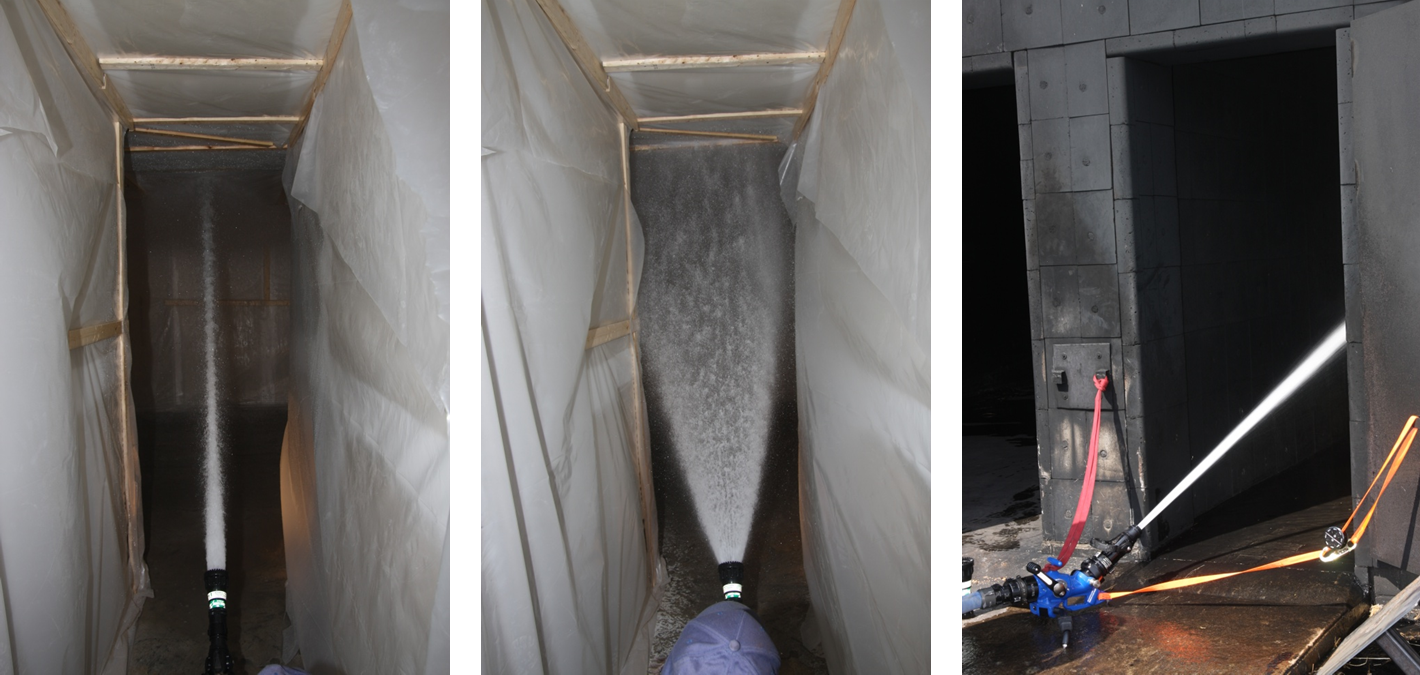
\includegraphics[width=6in]{../Figures/Pictures/Flows}
	\caption{Spray Density Nozzle Patterns}
	\label{fig:Spray_Density_Nozzle_Patterns}
\end{figure}

\subsection{Gas Cooling}
\label{sec:desc_Gas_Cooling}

Eighty-eight experiments were conducted to study the effectiveness of cooling the upper gas layer in a space adjacent to the area of fire involvement. These tests examined five different hose stream patterns, two nozzle types, and both compressed air foam and water as the suppression agent. The focus of this experimental series was to study the impact of the test variables on interior conditions throughout the structure when suppression tactics were applied to a room adjacent to the fire room. Detailed discussion of the tests and results are in Section~\ref{sec:Gas_Cooling}.

\subsection{Fire Suppression}
\label{sec:desc_Fire_Suppression}

The fire suppression series included 18 tests in two single-story experimental structures and one two-story structure. Fourteen tests were conducted in the single story structures (7 tests in each structure) using both water and CAFS application as a suppression agent. The nozzle patterns were varied from straight stream to narrow fog. Two of the tests examined suppression tactics for attic fires in residential dwellings, one in each structure. For the attic tests, a smooth bore nozzle was used. The 4 two-story tests used both water and CAFS from a straight-stream nozzle.

\section{Experimental Facilities}
\label{sec:Experimental_Facility}

The series of tests described within this report were conducted at the Delaware County Emergency Services Training Center, located in Sharon Hill, PA. A burn building as well as two purpose built concrete structures are located on the grounds of the ESTC. The burn building was used for the gas cooling experiments and the purpose built concrete structures were used for the fire suppression experiments.

\subsection{Fire Training Structure}
\label{sec:Burn_Building}

The burn building is a live fire training structure with both a two story and three story section. The building is supported with reinforced concrete beams and columns. The floors and ceilings are also concrete with the interior walls constructed of cement block. The walls and ceiling of the burn rooms are protected with a 25~mm thick layer of calcium silicate insulation and is covered by a 50~mm thick concrete tile. The floor of the burn rooms is protected with fire brick. Tests were conducted in the two-story, two-room configuration which has overall dimensions of 6.5~m (21.3~ft) by 9.2~m (30.2~ft) (cf. Fig.~\ref{fig:Delaware_County,_PA_Burn_Building_Layout}).

\begin{figure}[!ht]
	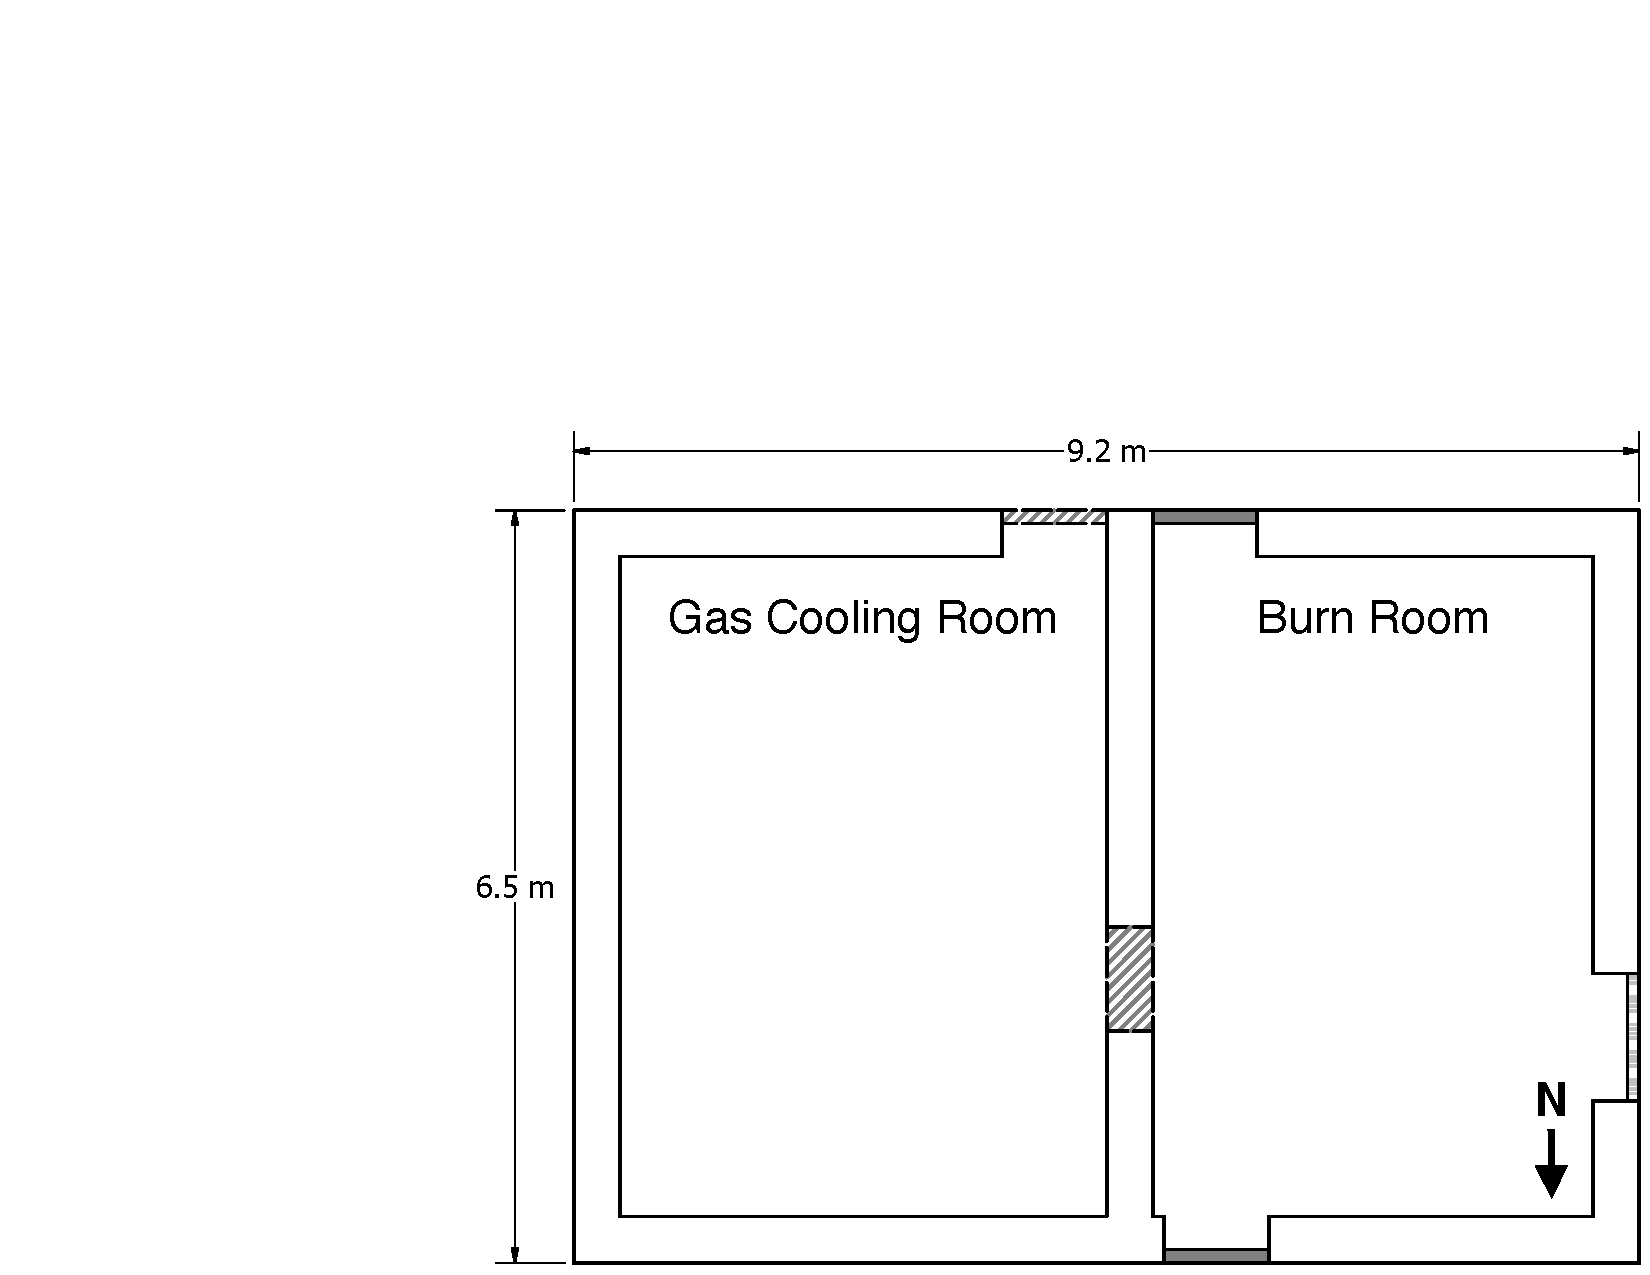
\includegraphics[width=\columnwidth]{../Figures/Floor_Plans/PDFs/West_Structure/DelCo_2012_West_Structure_Plain}
	\caption{Dimensioned Floor Plan Burn Building Layout}
	\label{fig:Delaware_County,_PA_Burn_Building_Layout}
\end{figure}

The burn room where the fuel load was located measured 3.8~m (12.5~ft) by 5.7~m (18.7~ft) with a ceiling height of 3.35~m (11.0~ft). The adjacent room where the water was applied for gas cooling measured 4.1~m (13.4~ft) by 5.7~m (18.7~ft), also with a ceiling height of 3.35~m (11.0~ft). The open door from the adjacent room to the exterior measured 2.0~m (6.5~ft) high and 0.9~m (2.9~ft) wide.

\subsection{Concrete Block Structures}
\label{sec:Experimental Structures}
\subsubsection*{Single Story Structures}

Two identical single story concrete structures were built on a concrete slab as shown in Fig.~\ref{fig:Delaware_County,_PA_Fire_Test_Structures}. They were designed to simulate a single floor of a residential structure.  The outer wall of each structure was composed of interlocking concrete blocks 0.61~m (2~ft) wide, 0.61~m (2~ft) high and 1.22~m (4~ft) long.  The interior dimensions of each structure were 6.1~m (20~ft) wide, 11~m (36~ft) long and 2.4~m (8~ft) high. The joints and gaps between the blocks were filled with high temperature insulation.

\begin{figure}[!ht]
	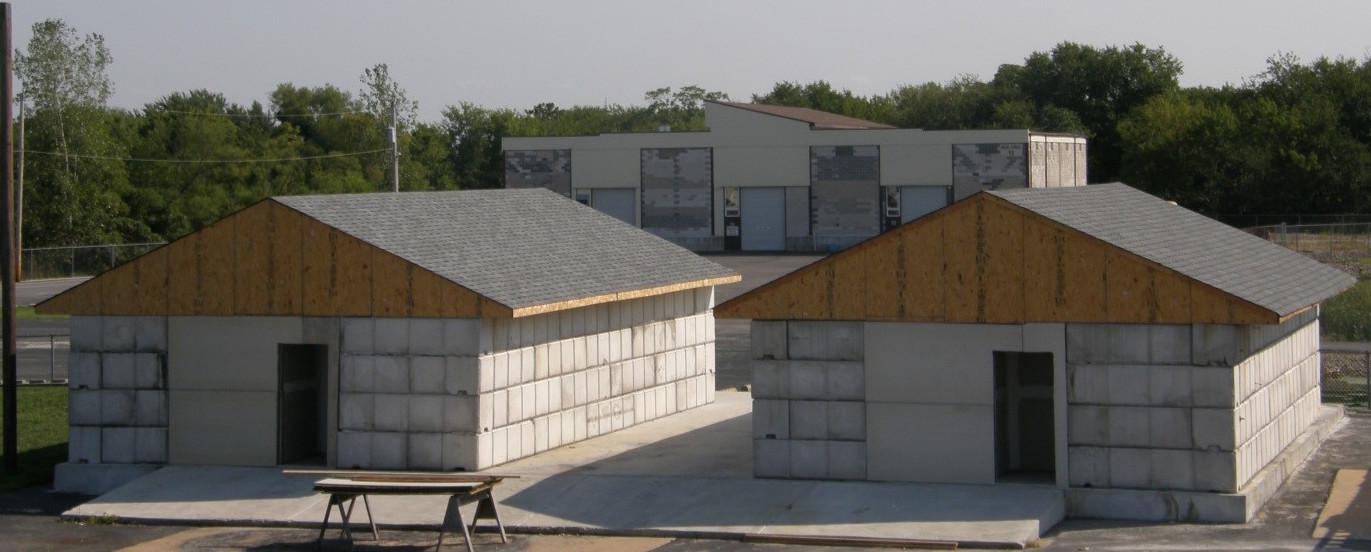
\includegraphics[width=6in]{../Figures/Pictures/DelCo_Structures}
	\caption{Delaware County, PA Fire Test Structures}
	\label{fig:Delaware_County,_PA_Fire_Test_Structures}
\end{figure}

Each structure had burn room, approximately 6.0~m (19.6~ft) by 4.4~m (14.3~ft) and 2.74~m (9.0~ft) in height and a hallway connecting the burn room to the front of the structure via a small entry foyer. The hallway was 0.95~m (3.1~ft) wide and 5.4~m (17.6~ft) long and the entry foyer was 1.2~m (4.1~ft) by 1.9~m (6.1~ft). The ceiling height in the hallway and entry foyer was 2.4~m (8~ft).  The open door on north side from the exterior to the entry foyer was 2.0~m (6.5~ft) high and 0.9~m (2.9~ft) wide. The opening on the south face of the structure from the exterior to the burn room was 2.4~m (7.75~ft) high and 1.09~m (3.6~ft) wide. A dimensioned, plan view of the structure is included in Fig.~\ref{fig:Test_Structure_Floor_Plan}.

\begin{figure}[!ht]
	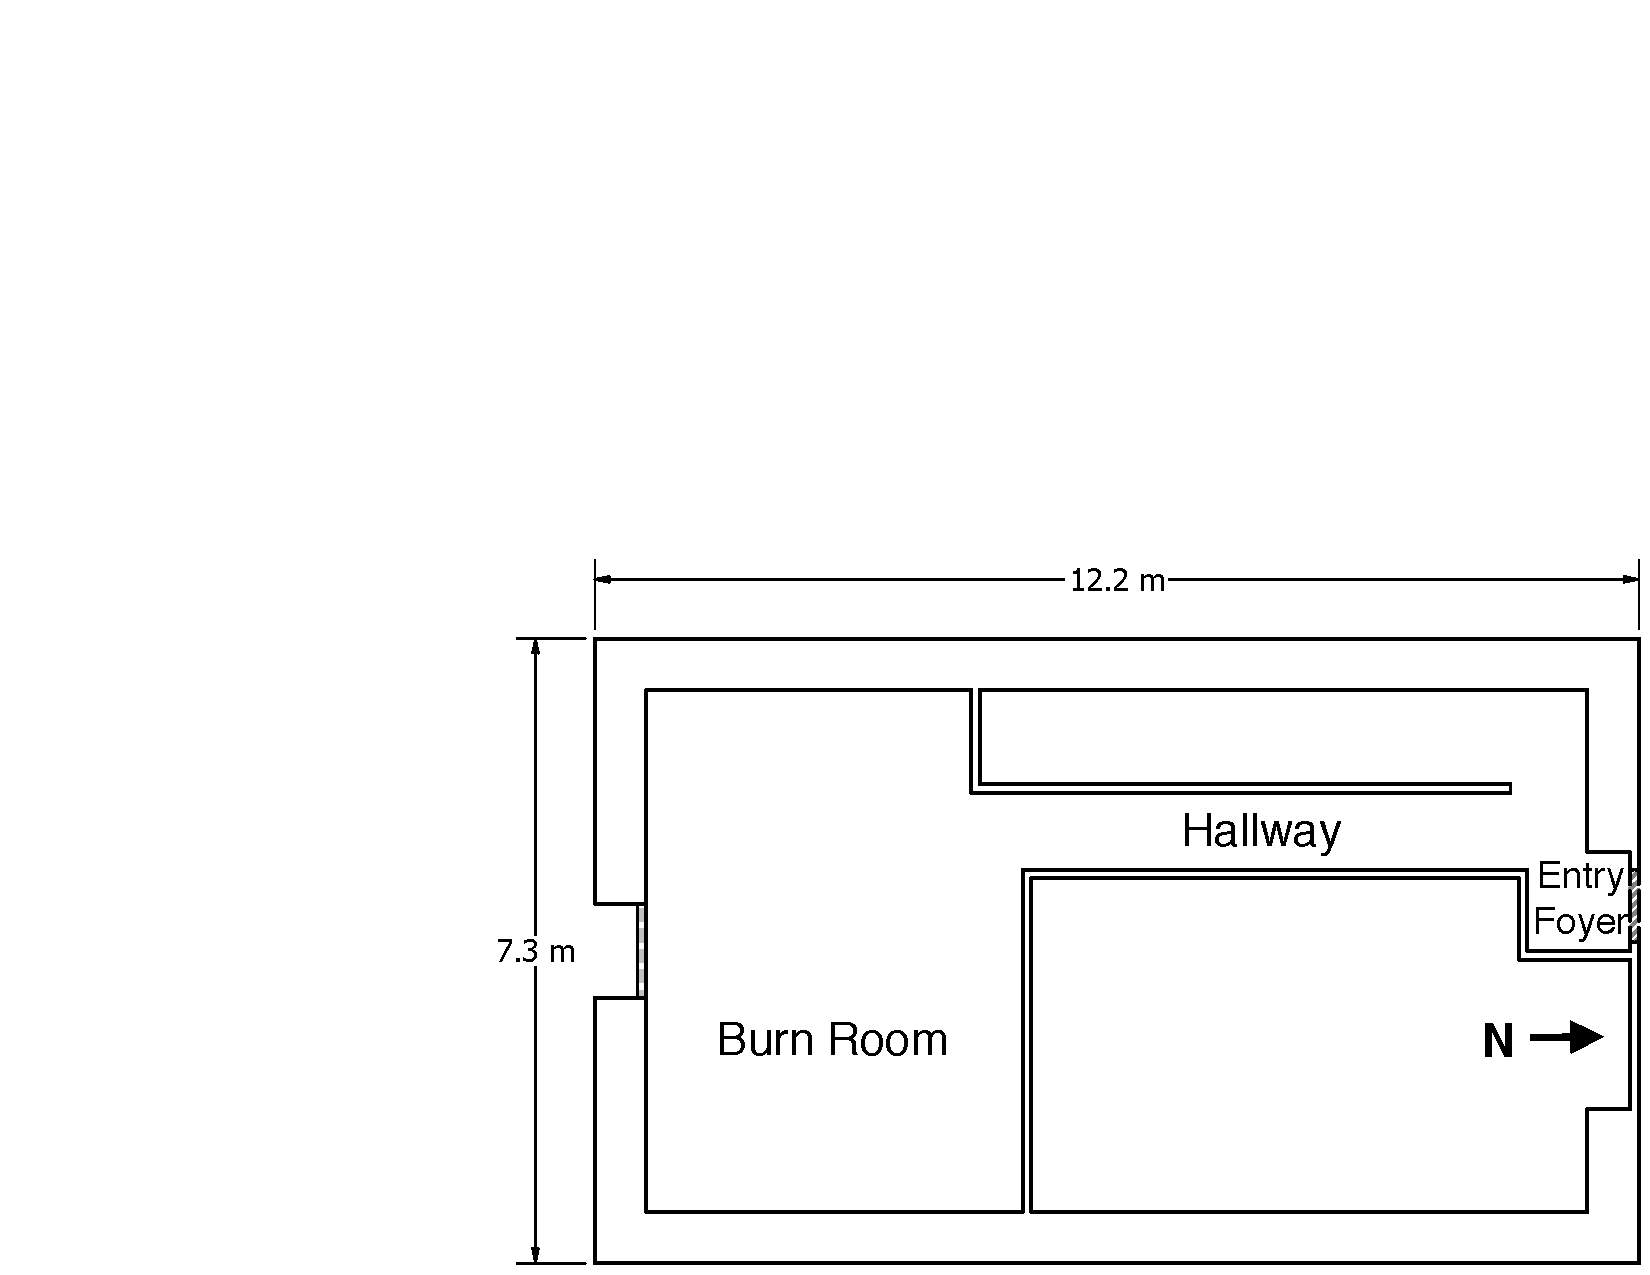
\includegraphics[width=\columnwidth]{../Figures/Floor_Plans/PDFs/East_Structure/DelCo_2012_East_Structure_Plain}
	\caption{Dimensioned Floor Plan of the Test Structure.}
	\label{fig:Test_Structure_Floor_Plan}
\end{figure}

The floor of the structure was the concrete pad. The interior walls of the structure were framed with steel studs and track.  The studs were set to 0.40~m (16~in) centers. The ceiling support was composed of wood truss joist I-beams (TJIs) with a 299~mm (11.75~in) depth. The TJI was composed of laminated veneer lumber flanges with a cross section of 29~mm (1.125~in) x 44~mm (1.75~in) and an 11~mm (0.43~in) thick oriented strand board web. Tongue and grove, 18.3~mm (0.72~in) thick, oriented strand board was attached to the top of the TJIs.

The interior walls of the burn room were lined with 13~mm (0.5~in) thick cement board. The ceiling of the burn room was the exposed ``floor assembly". The walls of the hallway and entry foyer were composed of 16~mm (0.625~in) Type X gypsum board. The ceiling of the hallway and entry foyer was composed of two layers of 13~mm (0.5~in) thick cement board.

\subsubsection*{Two Story Structure}

The west structure was modified to add second story to test larger fires and remote suppression effects (cf. Fig~\ref{fig:delco_2story}).

\begin{figure}[!ht]
	\includegraphics[width=6in]{../Figures/Pictures/DelCo}
	\caption{Delaware County, PA Fire Two-Story Test Structure}
	\label{fig:delco_2story}
\end{figure}

The outer walls of the bottom floor of the two-story structure were identical to that of the single story structures described above but with an open floor plan. The interior dimensions were 6.1~m (20~ft) wide, 11~m (36~ft) long and 2.4~m (8~ft) high. Figure~\ref{fig:dimensioned_first_2story} shows the dimensions of the reconfigured first floor. A stairwell was built to connect the floors. Stairs started 1.6~m (5.25~ft) off the South wall with a width of 1.2~m (4~ft) off the East wall. The second story walls were wood framed with 51~mm (2~in) by 102~mm (4~in) studs. The studs were set to 0.40~m (16~in) centers. The interior  walls were protected by 16~mm (5/8~in) fire rated gypsum board, 16~mm (5/8~in) durarock board, and a second layer of 16~mm (5/8~in) fire rated gypsum board. The exterior walls were protected with 11~mm (7/16~in) oriented strand board and 8~mm (5/16~in) fiber cement lap siding. Figure~\ref{fig:dimensioned_second_2story} shows the dimensions of the second story of the modified west structure.

\begin{figure}[!ht]
	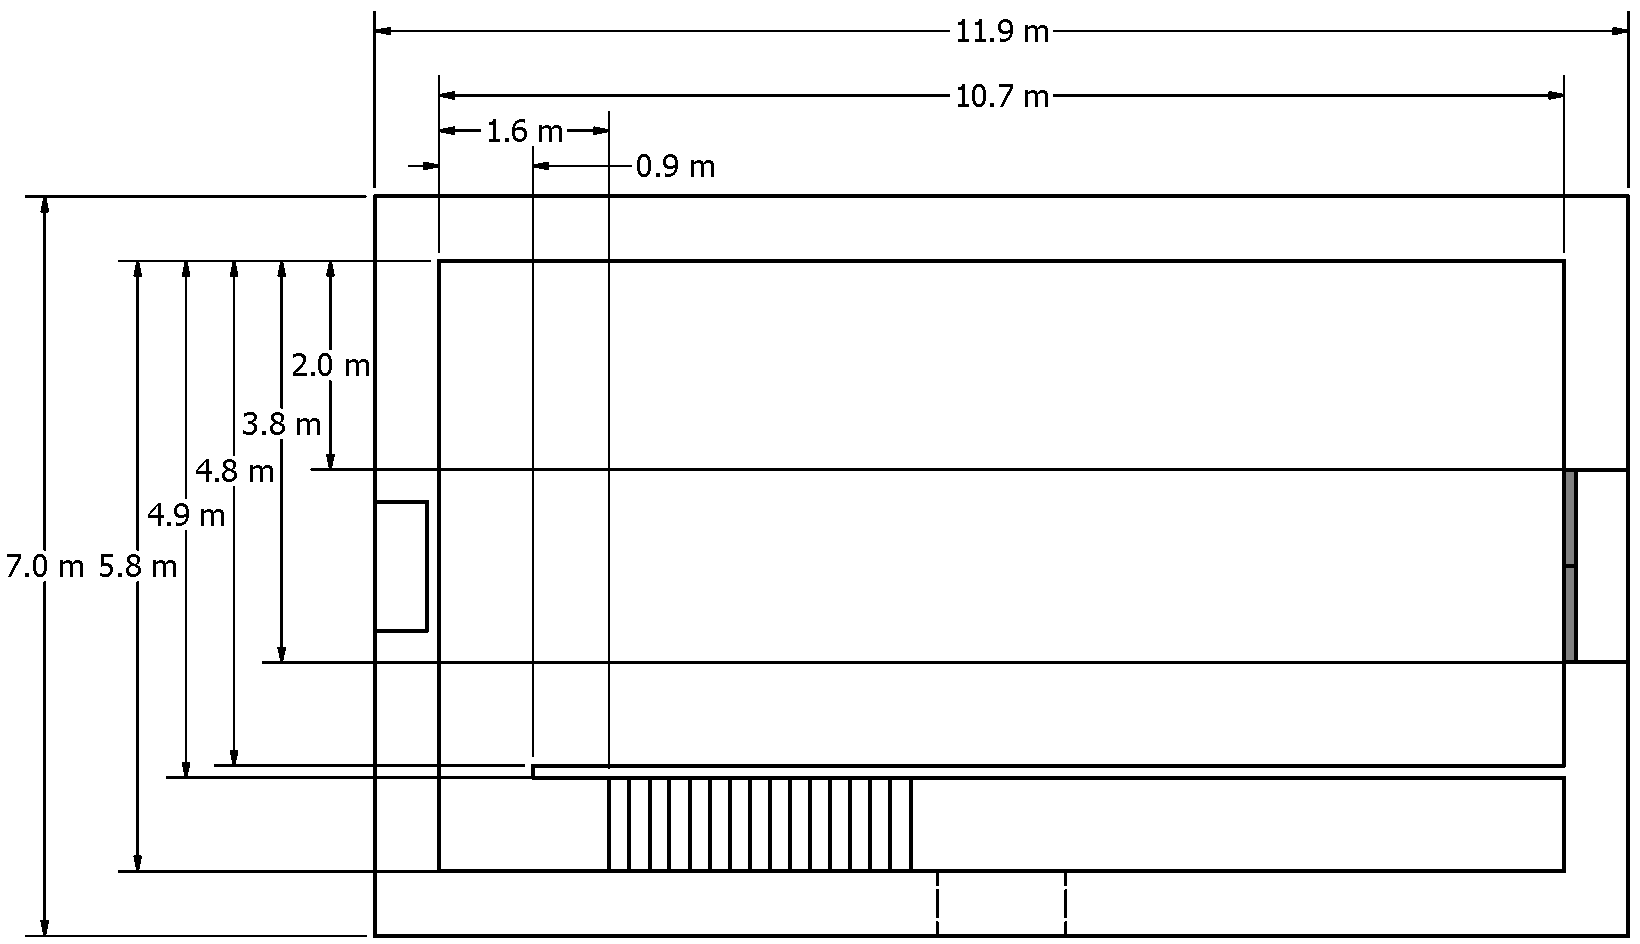
\includegraphics[width=\columnwidth]{../../DelCo_2014_2015/Drawings/PDFs/CAFS/West_Structure_1st_Floor_Plain}
	\caption{Dimensioned Floor Plan of First Floor of Two Story Structure.}
	\label{fig:dimensioned_first_2story}
\end{figure}


\begin{figure}[!ht]
	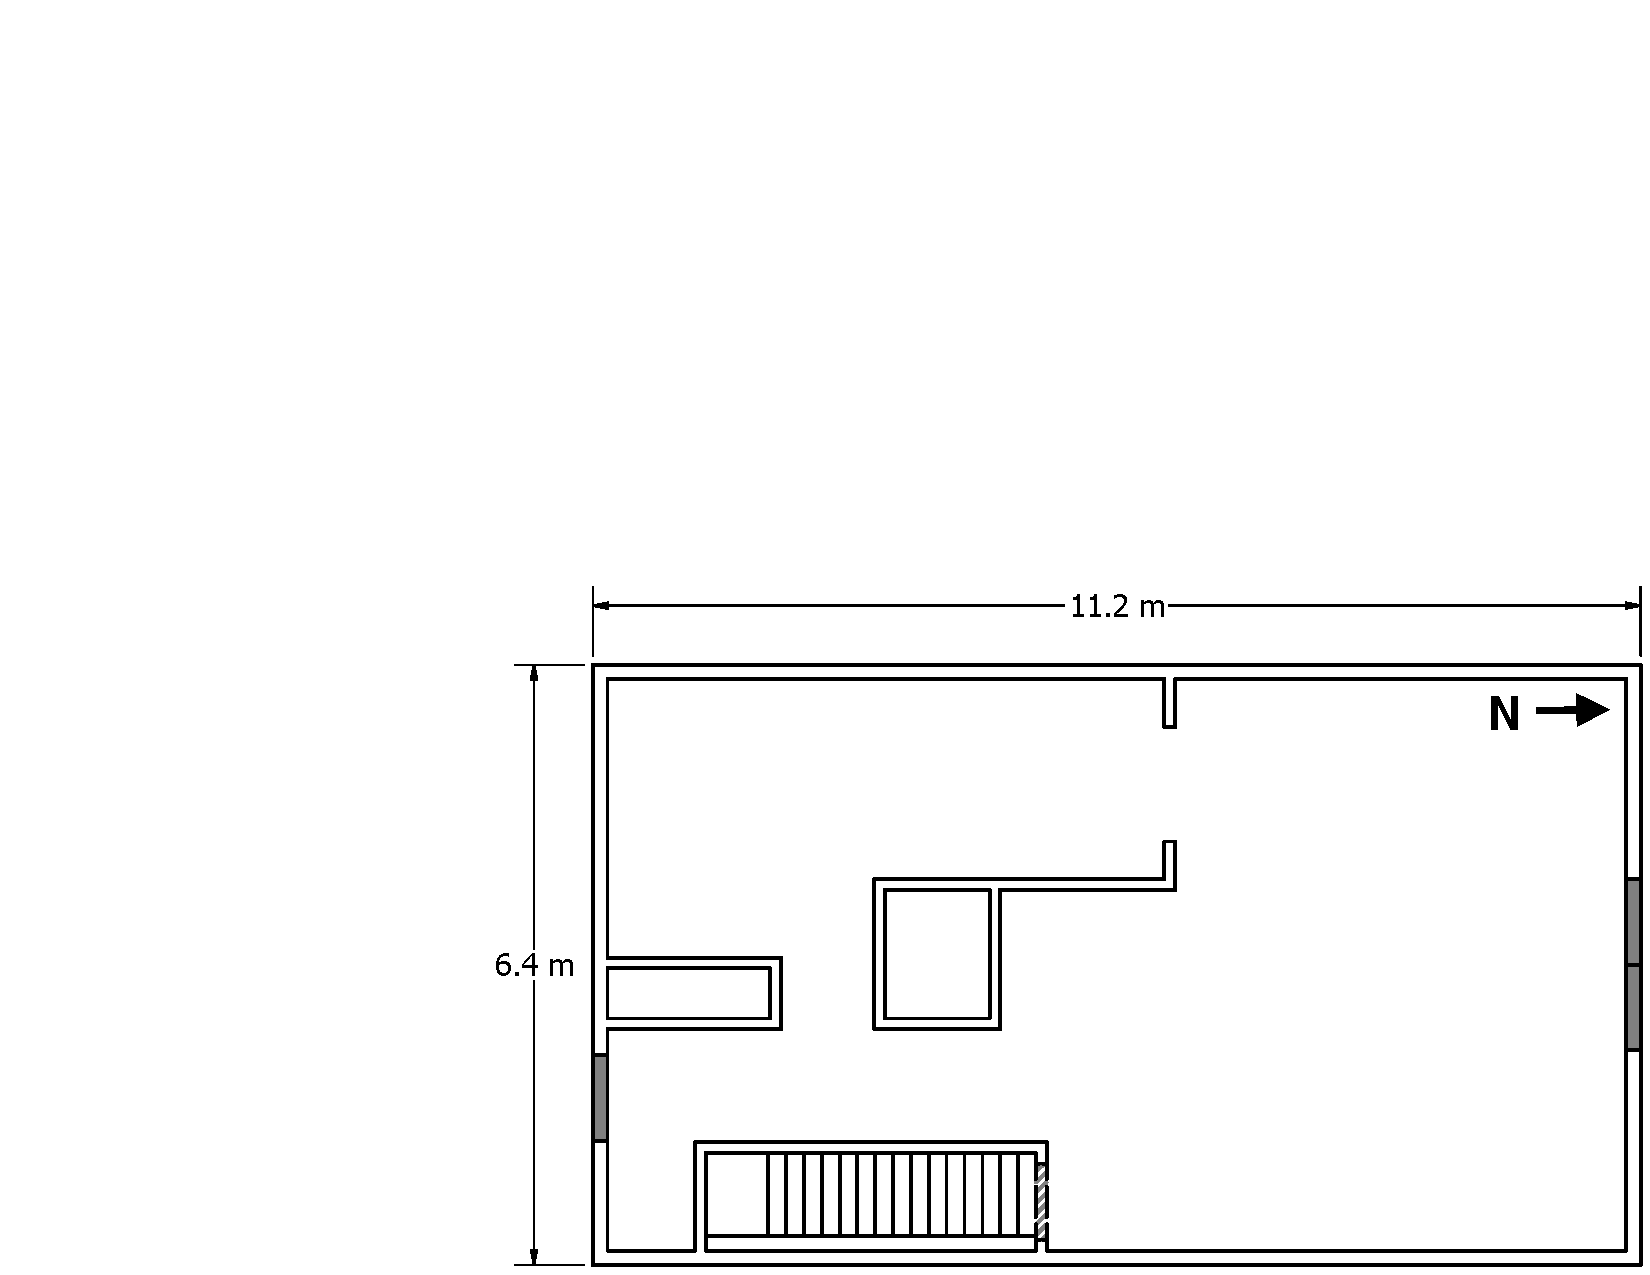
\includegraphics[width=\columnwidth]{../../DelCo_2014_2015/Drawings/PDFs/CAFS/West_Structure_2nd_Floor_Plain}
	\caption{Dimensioned Floor Plan of Second Floor of Two Story Structure.}
	\label{fig:dimensioned_second_2story}
\end{figure}

\clearpage

\section{Instrumentation}
\label{sec:Instrumentation}

The structures were instrumented for temperature, gas velocity, and heat flux measurements. Gas temperatures in the burn rooms were measured with bare-bead, Chromel-Alumel (type K) thermocouples. Additional single thermocouples were installed in conjunction with the bi-directional probes for gas velocity measurements. The single thermocouples were bare-bead, Chromel-Alumel (type K) thermocouples with a 1.0~mm (0.04~in) nominal diameter. The thermocouple wire was protected with an 3.2~mm (0.125~in) diameter inconel sheath. Schmidt-Boelter gauges were used to measure both total heat flux and radiant heat flux (radiometer). A radiometer is a total heat flux gauge with a zirconium plate to prevent contributions from convective heat transfer. A legend, which clarifies the instrumentation schematics discussed in the follow sections, is included in Fig.~\ref{fig:Instrumentation_Legend}.

\begin{figure}[!ht]
	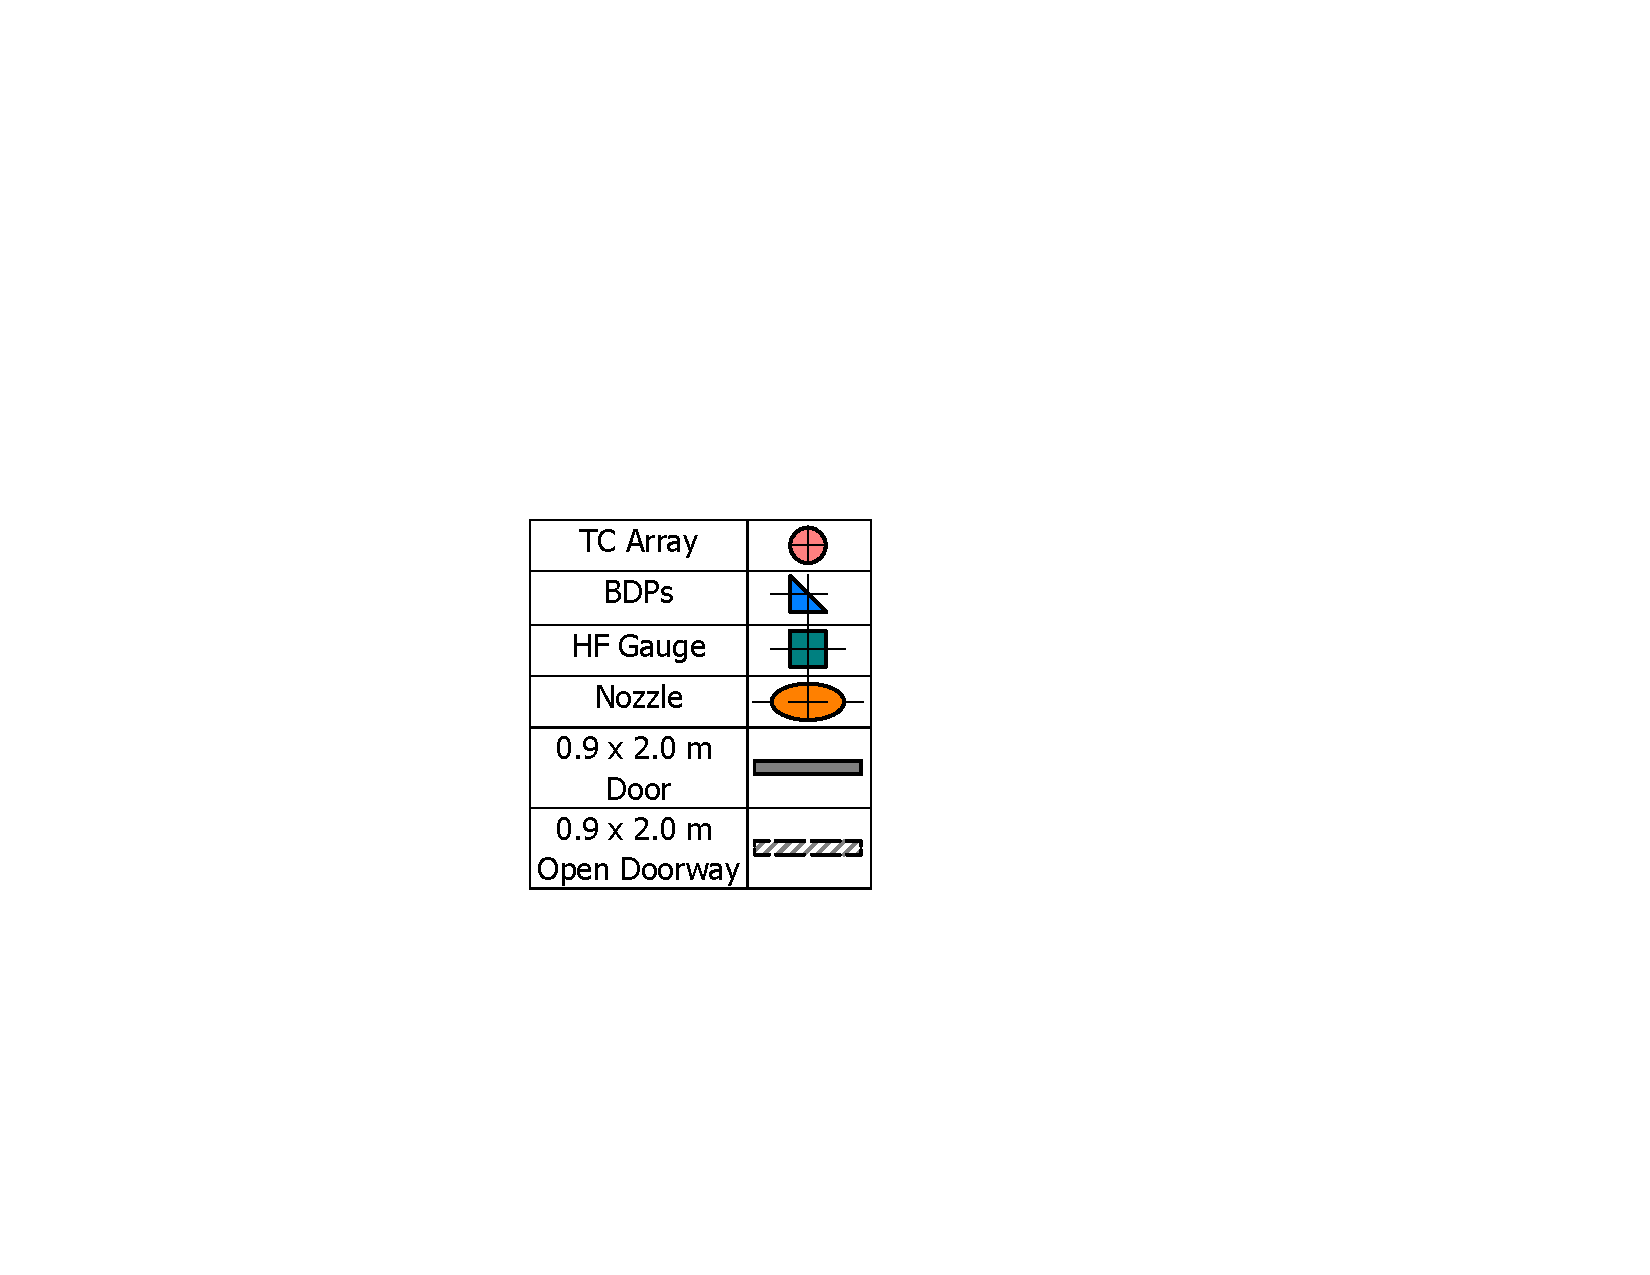
\includegraphics[width=.35\columnwidth]{../Figures/Floor_Plans/PDFs/DelCo_2012_Instrumentation_Legend.pdf}
	\caption{Instrumentation Legend.}
	\label{fig:Instrumentation_Legend}
\end{figure}

\subsection{Gas Cooling}
\label{subsec:Gas_Cooling_Instrumentation}

The gas cooling tests included 4 bare-bead thermocouple arrays  a bi-directional probe plus solid thermocouple array, and a total heat flux gauge/radiometer pair. Figure~\ref{fig:Gas_Cooling_Instrumentation_Dimensions} provides the positions within the burn room and gas cooling room where the senors were located (cf. Fig.~\ref{fig:Instrumentation_Legend} for reference on the symbols). Each of the bare-bead thermocouple array had 11 thermocouples. The top thermocouple was placed at the ceiling and each subsequent thermocouple was spaced 0.3~m (1~ft) apart with the bottom thermocouple being 3.05~m (10ft) below the ceiling. There were 6 velocity probes and solid thermocouples centered at the external doorway to the gas cooling room. The top probes were 0.15~m (0.5~ft) below the door soffit, the second probes were 0.3~m (1~ft), and the remaining 4 were spaced 0.3~m (1~ft) apart with the bottom probe being 1.52~m (5~ft) below the soffit. The total heat flux guage/radiometer were set to be 0.15~m (0.5~ft) off the ground and aimed to view the ceiling.

\begin{figure}[!ht]
	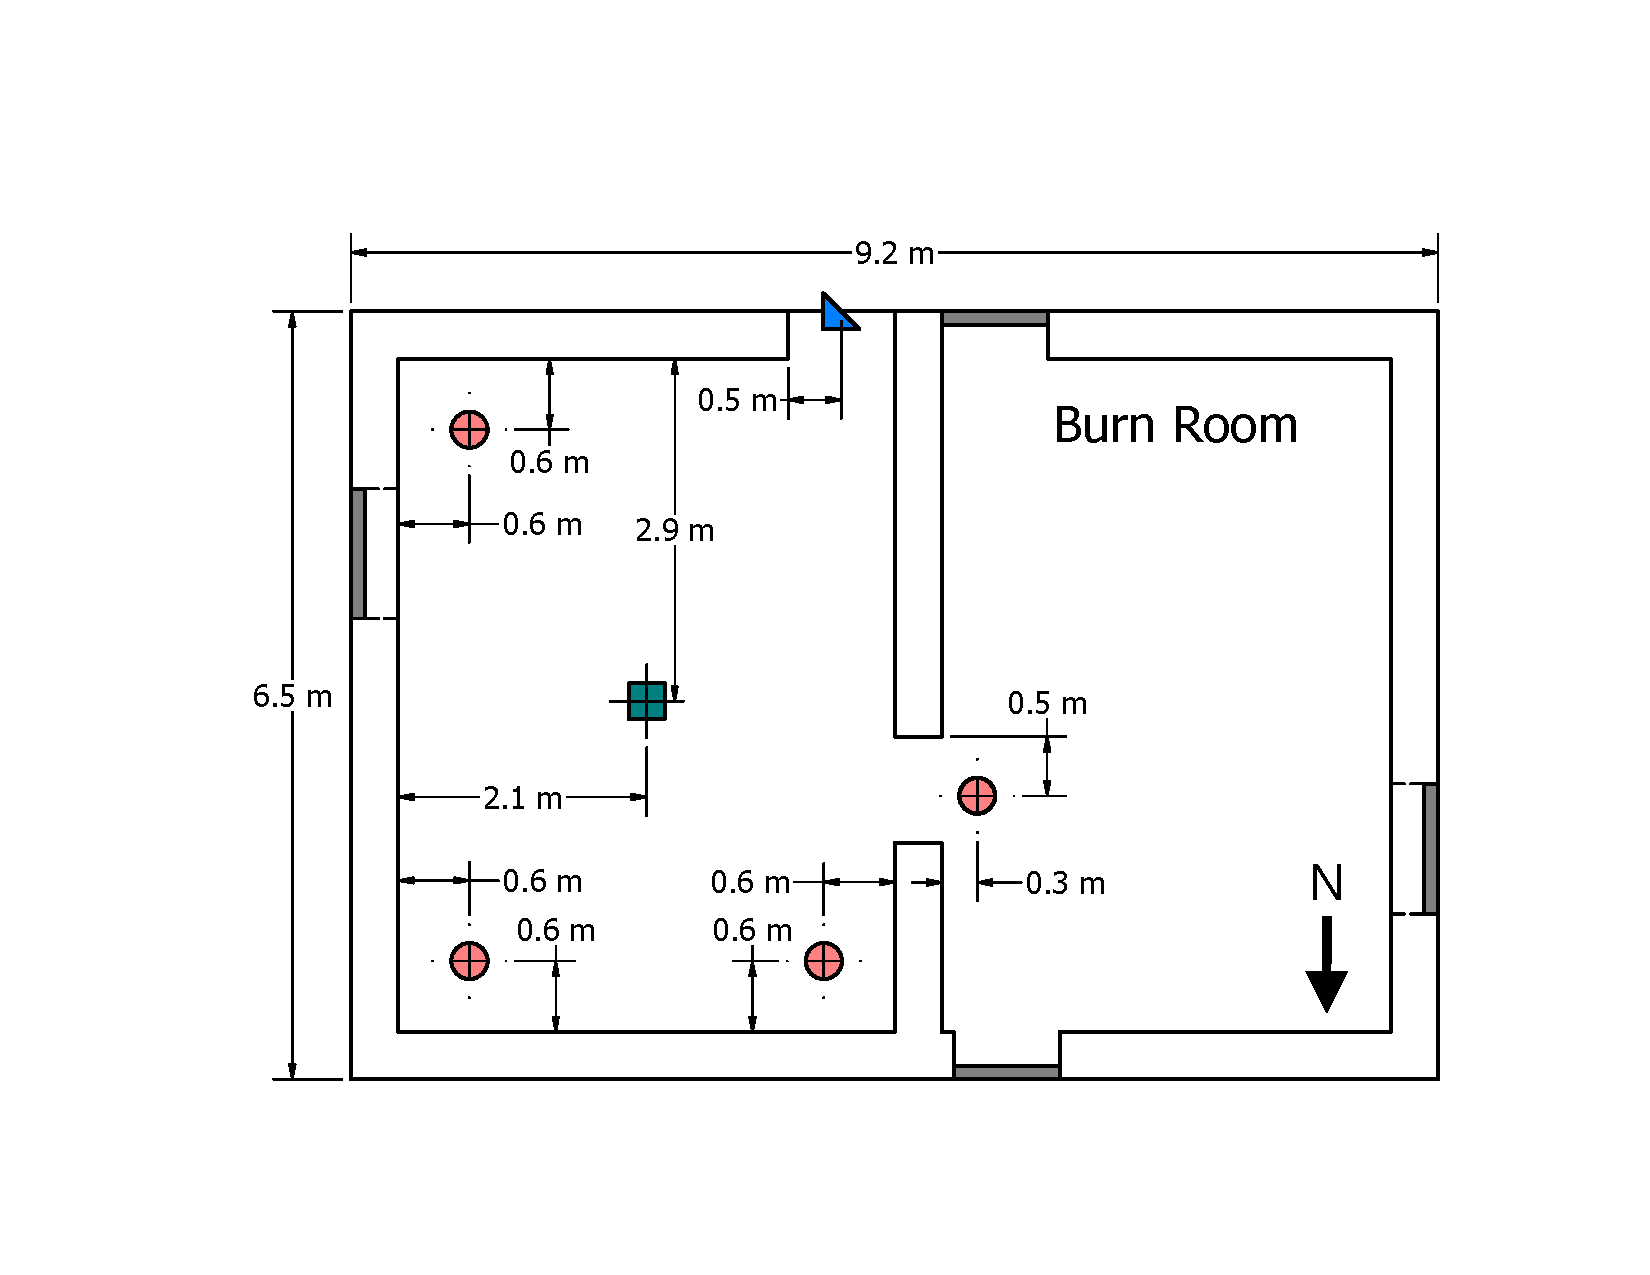
\includegraphics[width=\columnwidth]{../Figures/Floor_Plans/PDFs/West_Structure/DelCo_2012_West_Structure_Instrumentation}
	\caption{Instrumentation Schematic for the Gas Cooling Experiments.}
	\label{fig:Gas_Cooling_Instrumentation_Dimensions}
\end{figure}

\clearpage

\subsection{Fire Suppression}
\label{subsec:Fire_Suppression_Instrumentation}

\subsubsection*{Single Story Structure}

The fire suppression testing in the single story included 2 bare-bead thermocouple arrays, three bi-directional probe plus solid thermocouple arrays, 2 total heat flux gauge pairs, and 2 total heat flux guage/radiometer pairs. Figure~\ref{fig:Fire_Suppression_Instrumentation_Dimensions} provides the positions within the burn room, hallway, and entrance foyer where the senors were located (cf. Fig.~\ref{fig:Instrumentation_Legend} for reference on the symbols). Each bare-bead thermocouple array had 8 thermocouples. The top sensor was 0.03~m (1~in) below the ceiling and the remaining thermocouples were space 0.3~m (1~ft) apart with the bottom thermocouple being 2.13~m (7~ft) below the ceiling. The three bi-directional probe arrays had unique sensor locations. For the window array there were four sensor pairs located 0.28~m (0.95~ft), 0.58~m (1.90~ft), 0.84~m (2.85~ft), and 1.16~m (3.8~ft) below the soffit. For the hallway array, the 7 sensor pairs started 0.3~m (1~ft) below the ceiling and were spaced every 0.3~m (1~ft) ending 2.13~m (7~ft) below the ceiling. The doorway array also had 7 sensor pairs, but the first sensors were located 0.15~m (0.5~ft) below the soffit. The remaining sensors were spaced every 0.3~m (1~ft) with the bottom pair 1.83~m (6~ft) below the doorway soffit. The total heat flux guage/radiometer pairs were set to be 0.15~m (0.5~ft) off the ground and aimed to view the ceiling. The pairs of total heat flux guages were set 1~m (3~ft) off the ground with one sense ``looking'' vertical and the other horizontal.

\begin{figure}[!ht]
	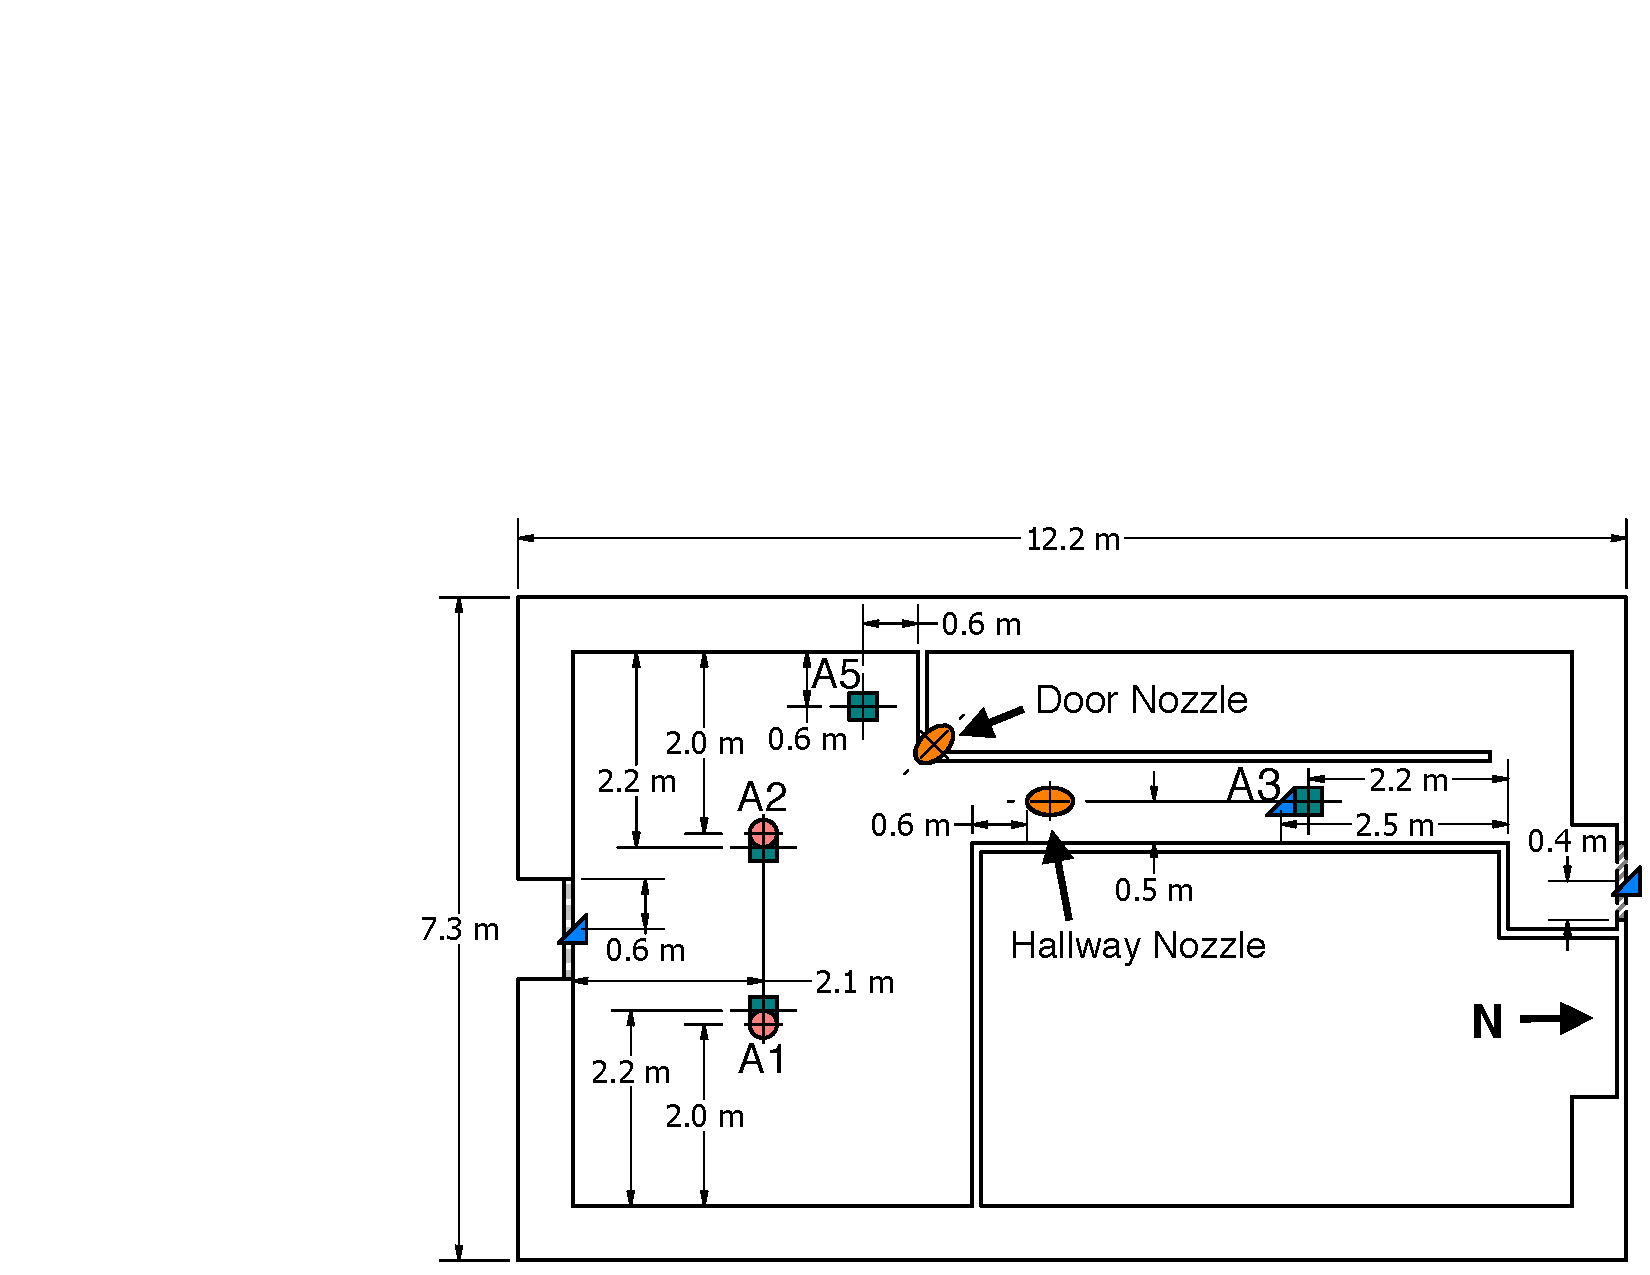
\includegraphics[width=\columnwidth]{../Figures/Floor_Plans/PDFs/East_Structure/DelCo_2012_East_Structure_Instrumentation}
	\caption{Instrumentation Schematic for the Single Story Fire Suppression Experiments.}
	\label{fig:Fire_Suppression_Instrumentation_Dimensions}
\end{figure}

\subsubsection*{Two Story Structure}

Fire suppression testing in the two-story structure included similar types instrumentation but included more sensors. Three bare-bead thermocouple arrays and 2 bi-directional probe plus solid thermocouples arrays were used in the first floor. Fig.~\ref{fig:fire_supp_first_2story} shows the positions of the instrumentation (cf. Fig.~\ref{fig:Instrumentation_Legend} for reference on the symbols). Each of the bare-bead arrays had 8 thermocouples with the same spacing as the single-story tests. The bi-directional probe and solid thermocouple arrays also had 8 sensors with the first probe 0.08~m (0.25~ft) below the soffit with the remaining probes at 0.34~m (1.1~ft), 0.61~m (2~ft), 0.88~m (2.9~ft), 1.15~m (3.7~ft), 1.42~m (4.7~ft), 1.68~m (5.5~ft), and 1.95~m (6.4~ft) below the soffit.

\begin{figure}[!ht]
	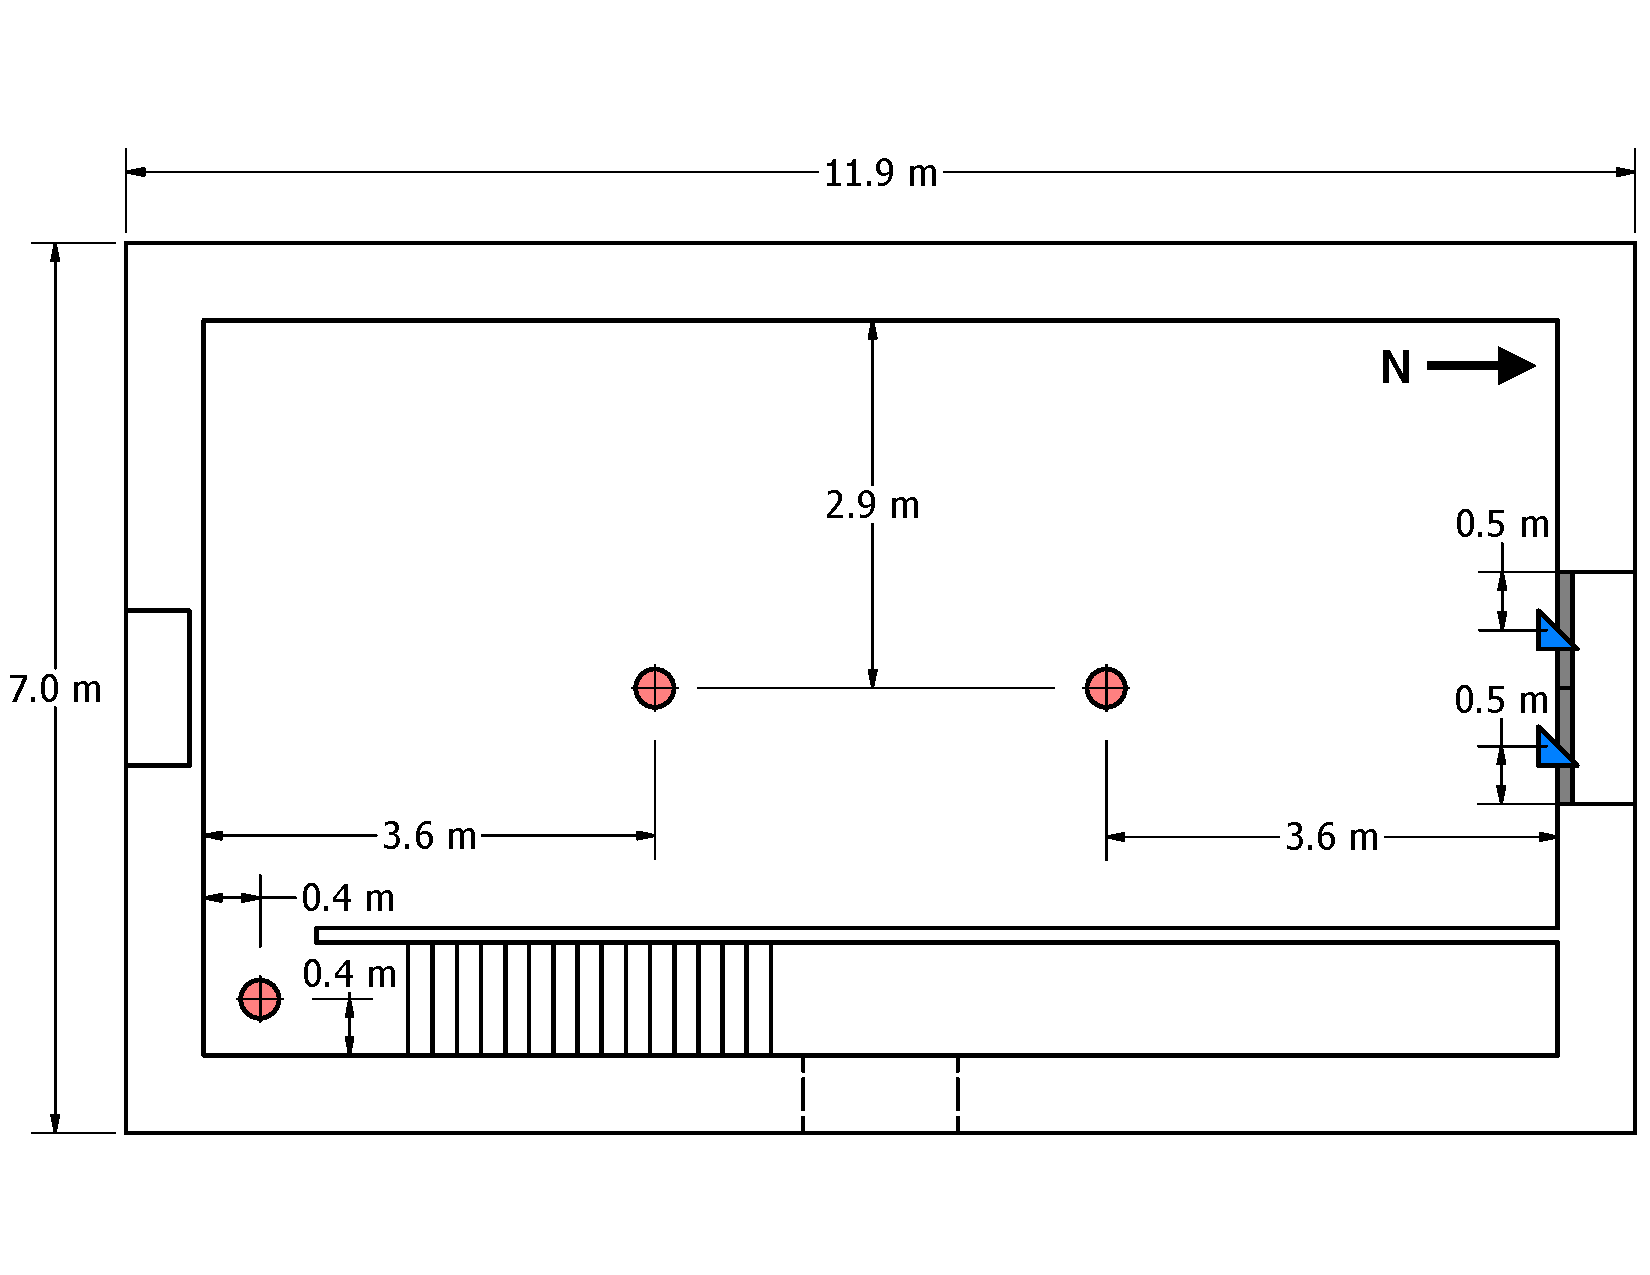
\includegraphics[width=\columnwidth]{../../DelCo_2014_2015/Drawings/PDFs/CAFS/West_Structure_1st_Floor_Instrumentation}
	\caption{Instrumentation Schematic for the First Floor of Fire Suppression Experiments in Two Story Structure.}
	\label{fig:fire_supp_first_2story}
\end{figure}

The second story featured 6 bare-bead arrays and 3 bi-directional probe plus solid thermocouple arrays. The second floor also had three heat flux sensor pairs (one facing horizontal and one facing vertical) that were 1~m (3~ft) off the ground. Fig.~\ref{fig:fire_supp_second_2story} shows the positions of the instrumentation (cf. Fig.~\ref{fig:Instrumentation_Legend} for reference on the symbols). The bare-bead thermocouple arrays featured 8 sensors with the same spacing as the basement level. The bi-direction probe arrays at the south wall door and at the top of the stairwell were comprised of 8 sensor pairs with the same spacing as the basement level. The third bi-directional probe array (3~m (9~ft) off the North wall and 0.6~m (2~ft) off the East wall) has 8 sensor pairs with the same spacing at the bare-bead thermocouple arrays.

\begin{figure}[!ht]
	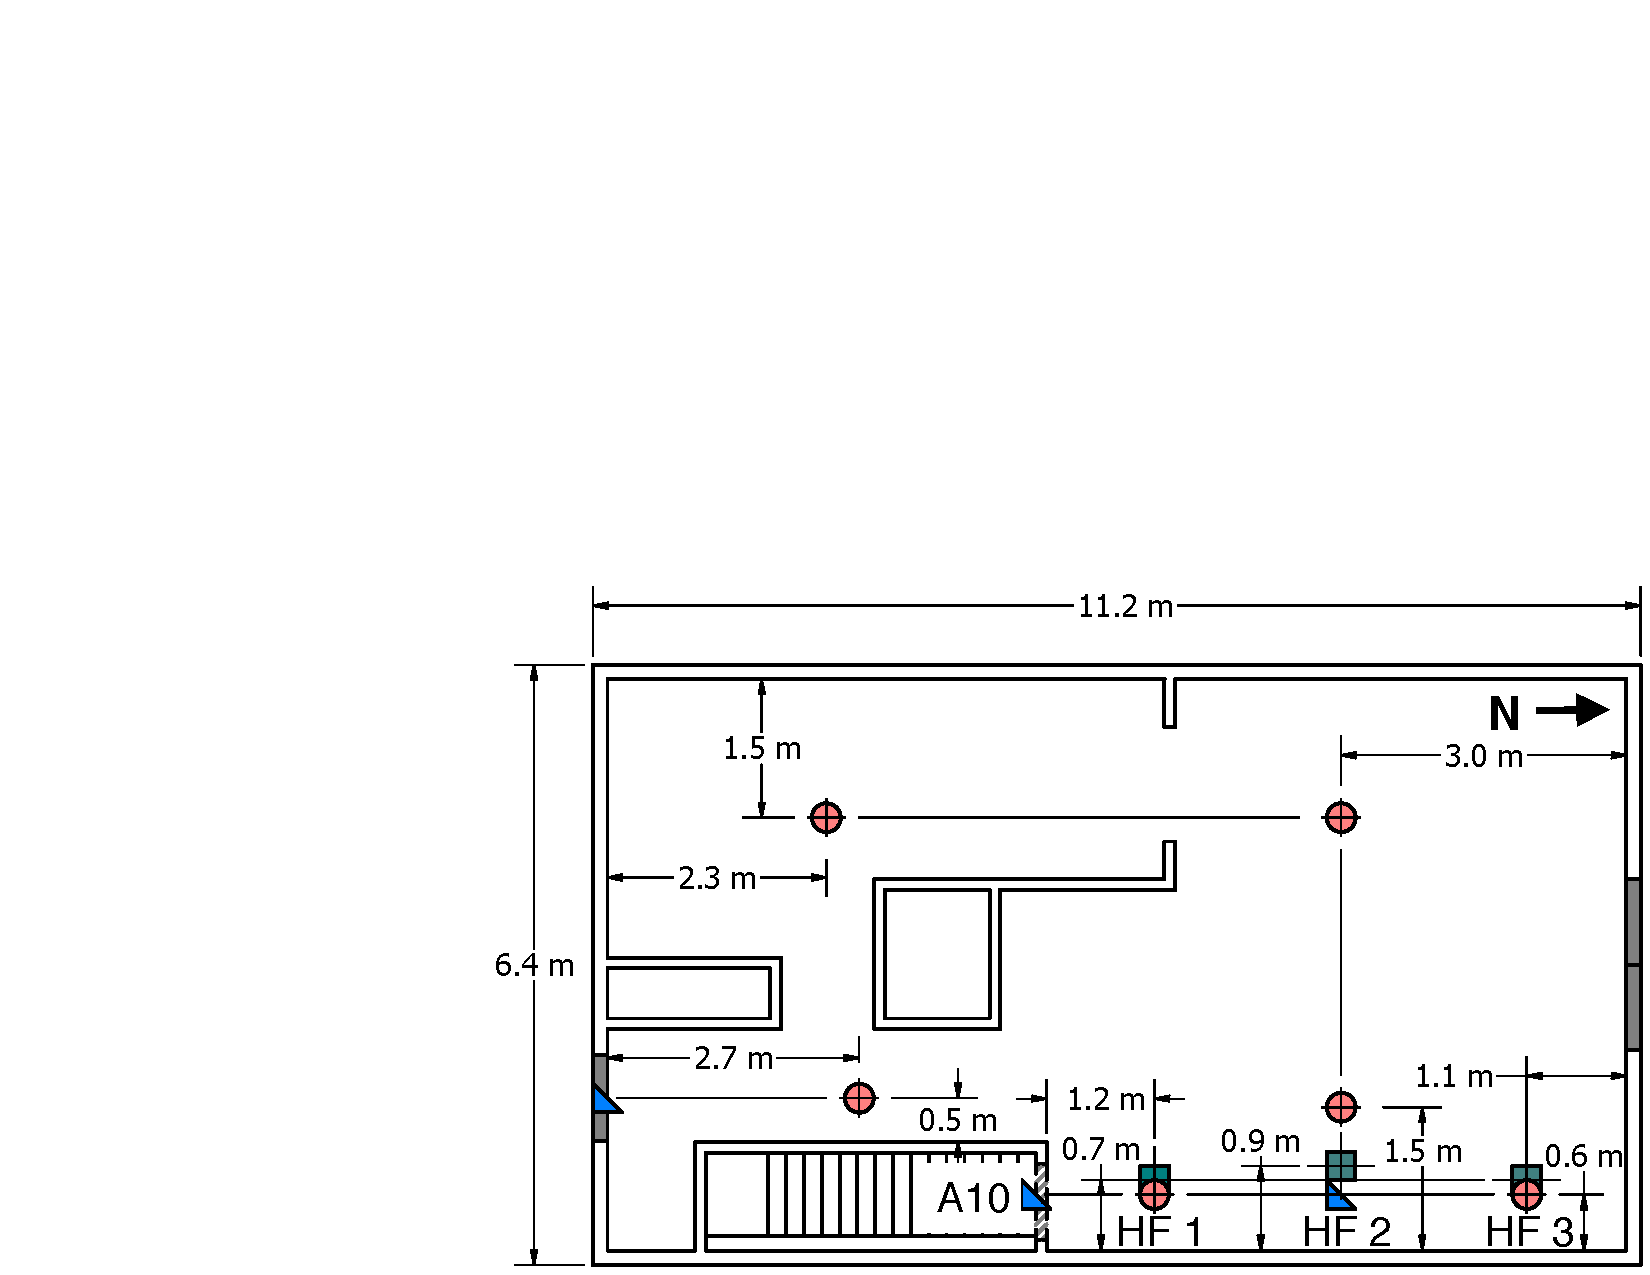
\includegraphics[width=\columnwidth]{../../DelCo_2014_2015/Drawings/PDFs/CAFS/West_Structure_2nd_Floor_Instrumentation}
	\caption{Instrumentation Schematic for the Second Floor of Fire Suppression Experiments in Two Story Structure.}
	\label{fig:fire_supp_second_2story}
\end{figure}

\clearpage

\subsection{Measurement Uncertainty}
\label{subsec:Uncertainty}

There are different components of uncertainty in the length, mass, temperature, heat flux, gas concentration, differential pressure, gas velocity and heat release rate reported here. Uncertainties are grouped into two categories according to the method used to estimate them. Type A uncertainties are those which are evaluated by statistical methods, and Type B are those which are evaluated by other means~\cite{Taylor&Kuyatt:1994}. Type B analysis of systematic uncertainties involves estimating the upper (+ a) and lower (- a) limits for the quantity in question such that the probability that the value would be in the interval ($\pm$ a) is essentially 100~\%. After estimating uncertainties by either Type A or B analysis, the uncertainties are combined in quadrature to yield the combined standard uncertainty. Then the combined standard uncertainty is multiplied by a coverage factor of two, which results in the expanded uncertainty with a 95~\% confidence interval (2$\sigma$).  For some of these components, such as the zero and calibration elements, uncertainties are derived from referenced instrument specifications. For other components, referenced research results and past experience with the instruments provided input in the uncertainty determination.

Each length measurement was taken carefully. Length measurements such as the room dimensions, instrumentation array locations and fire apparatus (for example nozzle, sprinkler, or fan) placement were made with a hand held laser measurement device which has an accuracy of $\pm$ 6.0~mm (0.25~in) over a range of 0.61~m (2.00~ft) to 15.3~m (50.0~ft)~\cite{StanleyTools}. However, conditions affecting the measurement, such as levelness of the device, yields an estimated uncertainty of $\pm$ 0.5~\% for measurements in the 2.0~m (6.6~ft) to 10.0~m (32.8~ft) range.  Steel measuring tapes with a resolution of  $\pm$ 0.5~mm (0.02~in) were used to locate individual sensors within a measurement array and to measure and position the furniture. The steel measuring tapes were manufactured in compliance with NIST Manual 44, which specifies a tolerance of $\pm$ 1.6~mm (0.06~in) for 9.1~m (30~ft) tapes and $\pm$ 6.4~mm (0.25~in) for 30.5~m (100~ft) tapes~\cite{Butcher:2012}. Some issues, such as ``soft'' edges on the upholstered furniture, result in an estimated total expanded uncertainty of $\pm$ 1.0~\%.

The load cell used to weigh the fuels prior to the experiments had a range of 0~kg (0~lb) to 200~kg (440~lb) with a resolution of a 0.05~kg (0.11~lb) and a calibration uncertainty within 1~\%~\cite{Ohaus:2000}. The expanded uncertainty is estimated to be less than $\pm$ 5~\%.

The standard uncertainty in temperature of the thermocouple wire itself is $\pm$ 2.2 $^{\circ}$C at 277 $^{\circ}$C and increases to $\pm$ 9.5~$^{\circ}$C at 871~$^{\circ}$C as determined by the wire manufacturer\cite{Omega:2004}. The variation of the temperature in the environment surrounding the thermocouple is known to be much greater than that of the wire uncertainty~\cite{Blevins:1999,Pitts:2003}. Small diameter thermocouples were used to limit the impact of radiative heating and cooling. The estimated total expanded uncertainty for temperature in these experiments is $\pm$ 15~\%.

In this study, total heat flux measurements were made with water-cooled Schimidt-Bolter gauges. The manufacturer reports a $\pm$ 3~\% calibration expanded uncertainty for these devices~\cite{Medtherm:2003}. Results from an international study on total heat flux gauge calibration and response demonstrated that the uncertainty of a Schmidt-Boelter gauge is typically $\pm$ 8~\%~\cite{Pitts:2006}.

The gas measurement instruments and sampling system used in this series of experiments have demonstrated an expanded (k = 2) relative uncertainty of $\pm$ 1~\% when compared with span gas volume fractions~\cite{Bundy:2007}. Given the non-uniformities and movement of the fire gas environment and the limited set of sampling points in these experiments an estimated uncertainty of $\pm$ 12~\% is being applied to the results~\cite{Lock:1}.

Differential pressure reading uncertainty components were derived from pressure transducer instrument specifications and previous experience with pressure transducers. The transducers were factory calibrated and the zero and span of each was checked in the laboratory prior to the experiments yielding an accuracy of $\pm$ 1~\%~\cite{Setra:2002}. The total expanded uncertainty was estimated at 10~\%.

Bi-directional probes and single thermocouples were used to measure the velocity. The bi-directional probes used similar pressure transducers as those used for the differential pressure measurements discussed above. Bare-bead Type K thermocouple are co-located with the probe. A gas velocity measurement study examining the doorway flow of pre-flashover compartment fires yielded expanded uncertainty measurements ranging from $\pm$ 0.14 to $\pm$ 0.22 for bi-directional probes of similar design~\cite{Bryant:FSJ2009}. The total expanded uncertainty for gas velocity in these experiments was estimated to be $\pm$ 18~\%.

Water flowrate was measured with a pressure and flow meter combination. The meter consists of a section of 6.35~cm (2.5~inch) cast aluminum pipe with a 0 - 4.1~MPa (0 - 600~psi) pressure transducer and a paddlewheel type flow sensor with a range of 0 to 4800~lpm (1250~gpm). The pressure transducer and paddlewheel both connect to the battery operated control box where the pressure transducer voltage is converted to a pressure and the paddlewheel pulse count is converted to a volumetric flow rate.  The manufacturer reports a $\pm$ 5~\% calibration expanded uncertainty for the flow sensor and $\pm$ 3~\%  for the pressure sensor~\cite{Akron:2009}. The pressure transducer was calibrated with a known analog pressure gauge. The flow meter was calibrated by capturing water over time and measuring that mass of water to determine the flowrate. The total expanded uncertainty was estimated at $\pm$ 10~\%.

\section{Fuel Load}
\label{sec:fuel_load}

\subsection{Gas Cooling}
\label{sec:Fuel_Load_Gas_Cooling}

Wood pallets were used as the fuel source for the gas cooling experiments. The pallets were approximately 1.2~m (4.0~ft) by 1.0~m (3.3~ft) by 0.13~m (0.42~ft) thick. The pallets ranged in mass from 13.6~kg (29.9~lb) to 26.4~kg (58.1~lb) with an average of 18.4~kg (40.5~lbs). The initial fuel load consisted of 10 pallets, arranged in two stacks of five as shown in Fig.~\ref{fig:Burn_Building_Fuel_Load}. Approximately one half of a bale of excelsior, 13.0~kg (28.6~lb), was mixed with the pallets to aid with ignition. Fig.~\ref{fig:Burn_Building_Fuel_Load}, also provides dimensioned locations of the two stacks of pallets within the burn room.

\begin{figure}[!ht]
	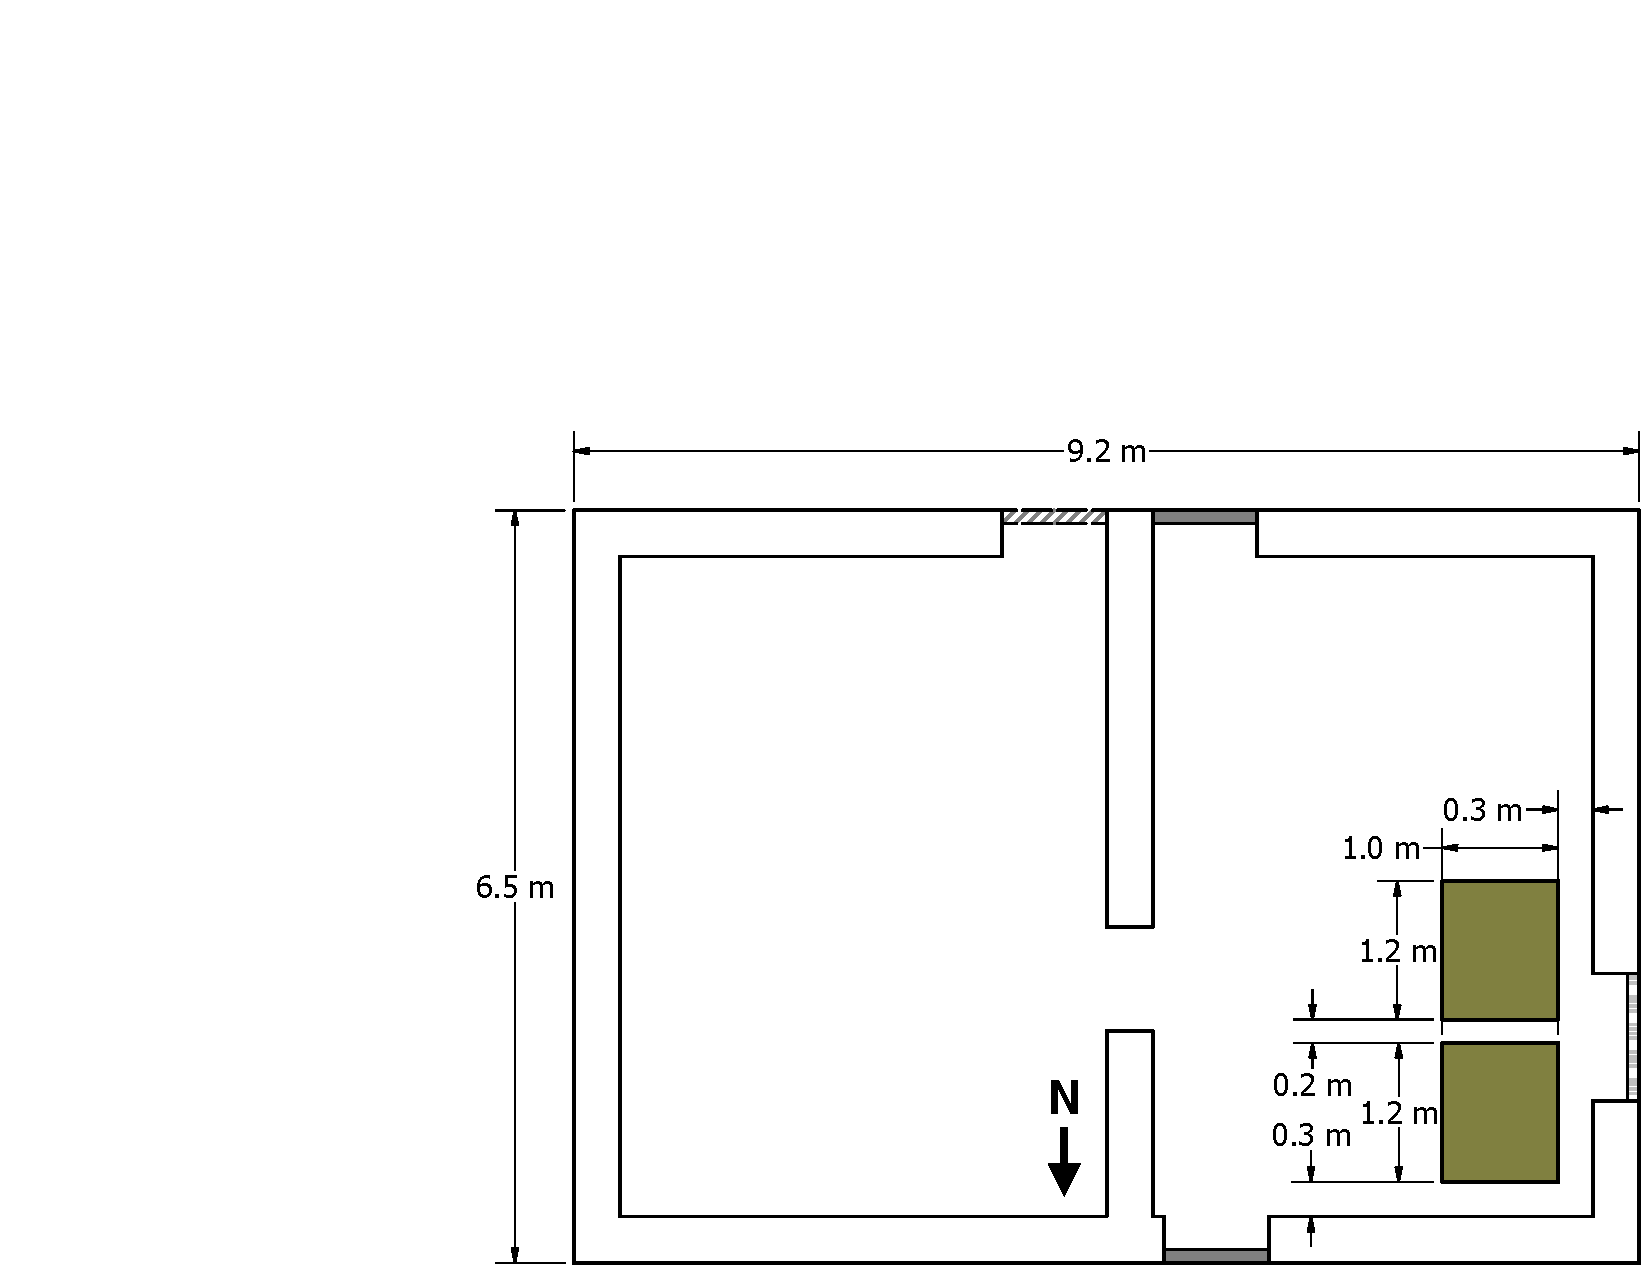
\includegraphics[width=\columnwidth]{../Figures/Floor_Plans/PDFs/West_Structure/DelCo_2012_West_Structure_Pallets}
	\caption{Burn Building Fuel Load.}
	\label{fig:Burn_Building_Fuel_Load}
\end{figure}

Note, that as the pallets burned away and the hot gas layer temperatures decreased, the steel shutters on the window to the burn room were opened and additional pallets were added. Pallets were added to the existing fuel locations until the flames from the piles reached the ceiling of the burn room again. The number of pallets added each time varied.

\clearpage

\subsection{Fire Suppression}
\label{sec:Fuel_Load_Fire_Suppression}

\subsubsection*{Single Story Structure}
\label{sec:suppresion_single}

\subsubsection{Wood Fuel Package}
\label{sec:fire_suppression_pallet_fuel}

The fuel load for these experiments consisted of one bale of hay, twelve pallets, eleven and a half sheets plywood on the walls and the wood ``floor assembly". Two stacks of pallets with hay were used as the first items ignited in each experiment. Each stack was composed of six pallets with a half bale of hay. The hay was layered between each pallet. Figure~\ref{fig:Wood_Fuel_Load} shows the pallets prior to ignition. The pallets and hay were weighed prior to each experiment. For the four pallet experiments, the average mass of the two stacks of pallets and the bale of hay was 232.4~kg (511.3~lb).
\begin{figure}[!ht]
	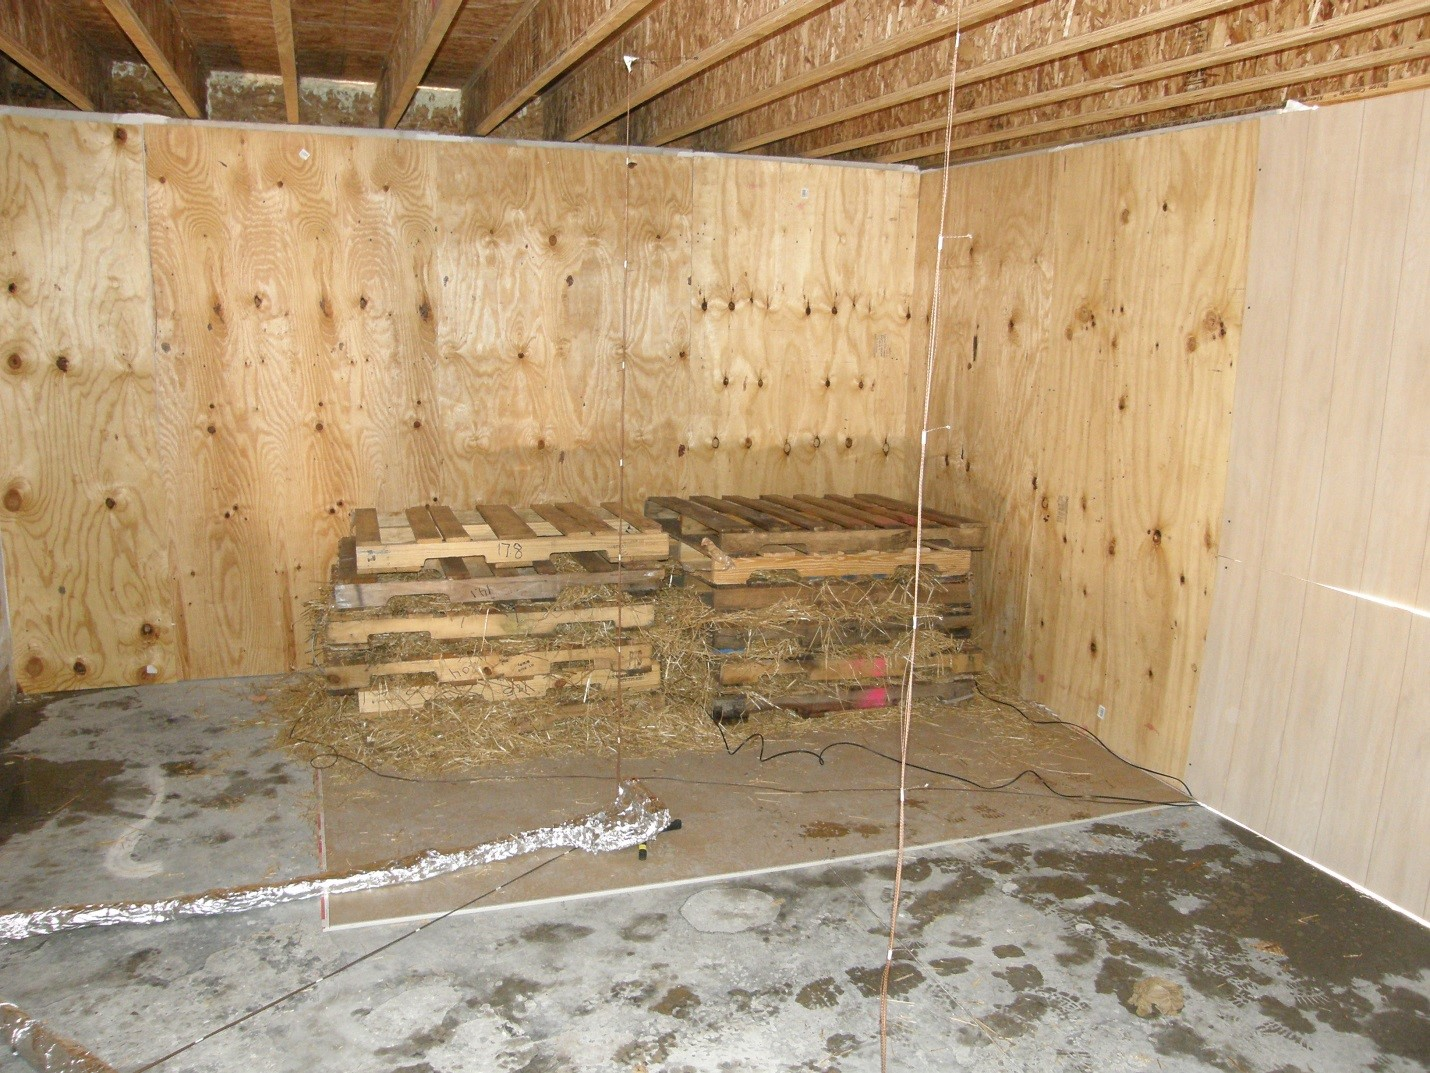
\includegraphics[width=0.65\columnwidth]{../Figures/Pictures/Wood_Fuel_Package}
	\caption{Photograph of Southeast corner of burn room with wood fuel load.}
	\label{fig:Wood_Fuel_Load}
\end{figure}

The pallet stacks were located 0.3~m (12~in) away from the east and south walls of the burn room (cf. Fig.~\ref{fig:Wood_Fuel_Load_Dimensions}). The pallets were 1.2~m (48~in) long, 1.0~m (40~in) and 123~mm (4.8~in) high. The stacks were spaced 150~mm (6~in) apart. One layer of 13~mm (0.5~in) thick gypsum board panels were laid on the concrete floor under the wood pallets to form a protective layer to minimize thermal damage to the concrete floor. The east and south wall of the burn room was covered with 15~mm (0.59~in) thick, sheets of plywood.  The ``wood flooring assembly", composed of 12 TGIs and 9 sheets of OSB, served as the ceiling of the burn room. The open doorway to the burn room on the south side was covered with a 2.4~m (8~ft) tall by 1.2~m (4~ft) wide piece of medium density fiberboard paneling that was 5~mm (0.19~in) thick.

\begin{figure}[!ht]
	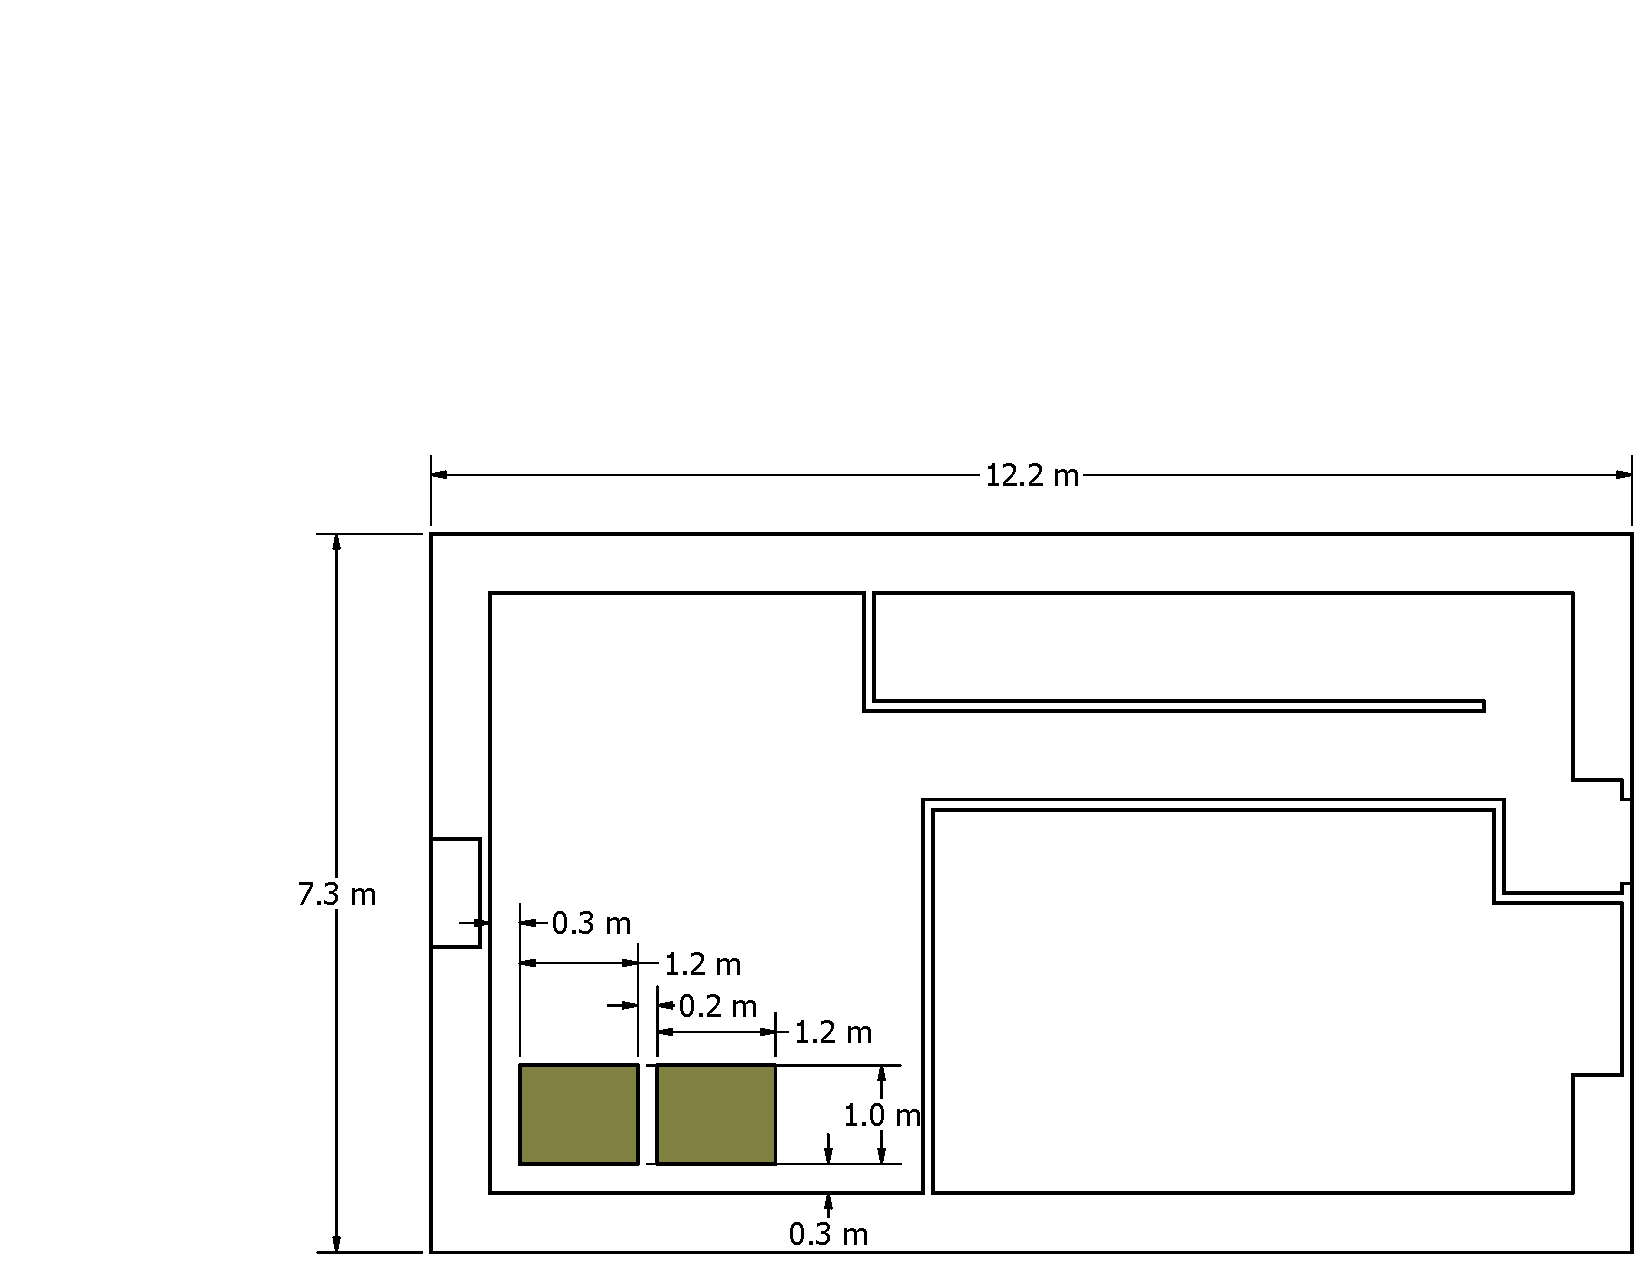
\includegraphics[width=.8\columnwidth]{../Figures/Floor_Plans/PDFs/East_Structure/DelCo_2012_East_Structure_Pallets}
	\caption{Wood Fuel Load in Single Story Structure.}
	\label{fig:Wood_Fuel_Load_Dimensions}
\end{figure}

\subsubsection{Furniture Fuel Package}
\label{sec:fire_suppression_furniture_fuel}

The fuel load for these experiments consisted of 2 sleeper sofas and 2 chairs, carpet, padding, and wood paneling along the southeast corner walls. An image of the fuel arrangement is shown in Fig.~\ref{fig:Furniture_Fuel_Load}. The couches and chairs are setup to mimic a typical seating area with one couch against the south and east wall respectively with each being 0.9~m (36~in) away from the corner. A chair is placed adjacent to each couch and the specific locations can be found in the dimensioned schematic, Fig.~\ref{fig:Furniture_Fuel_Load_Dimensions}. In total, this fuel package contains approximately 336 kg of fuel consisting of wood, polyurethane (PU), polyester (PET),and polypropylene (PP). Table~\ref{tab:Fire_Suppression_Fuel_Masses} provides a breakdown on the fuel composition for these experiments.

\begin{figure}[!ht]
	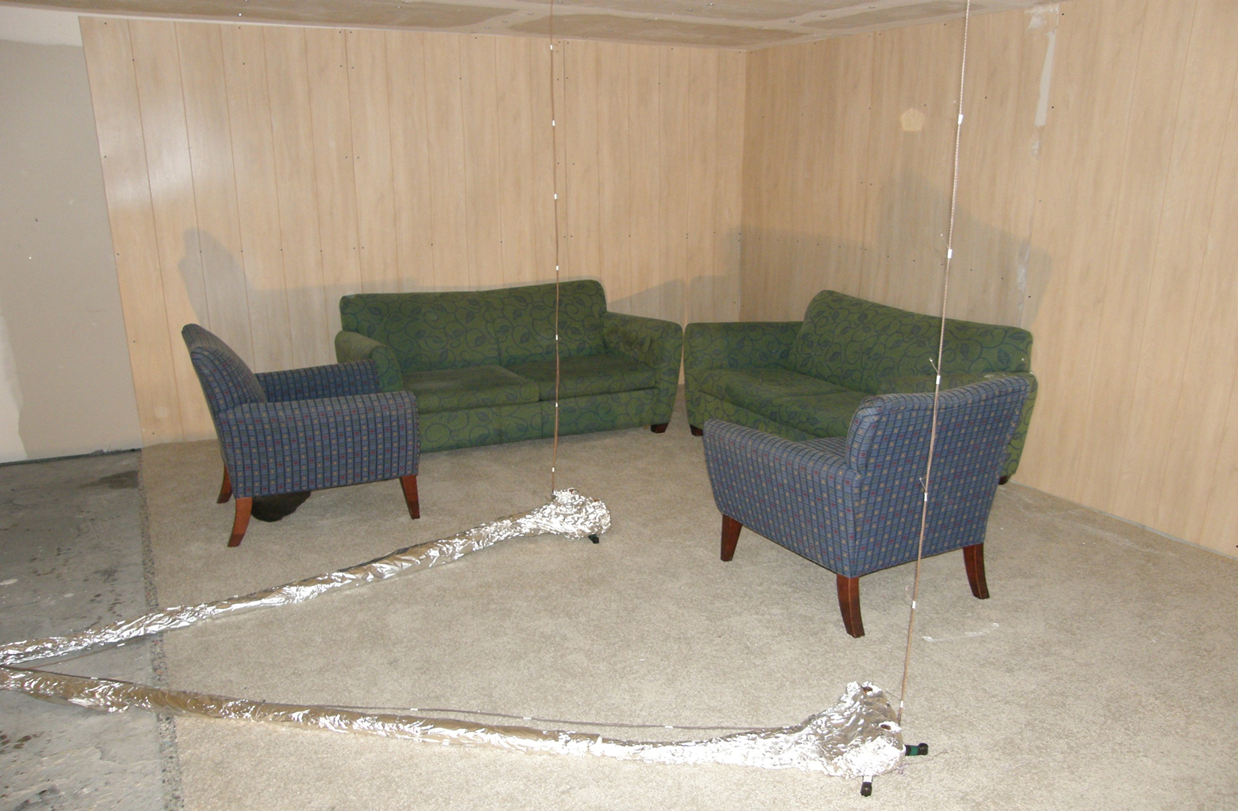
\includegraphics[width=.8\columnwidth]{../Figures/Pictures/Furniture_Fuel_Load}
	\caption{Furniture Fuel Load in Single Story Structure}
	\label{fig:Furniture_Fuel_Load}
\end{figure}

\begin{figure}[!ht]
	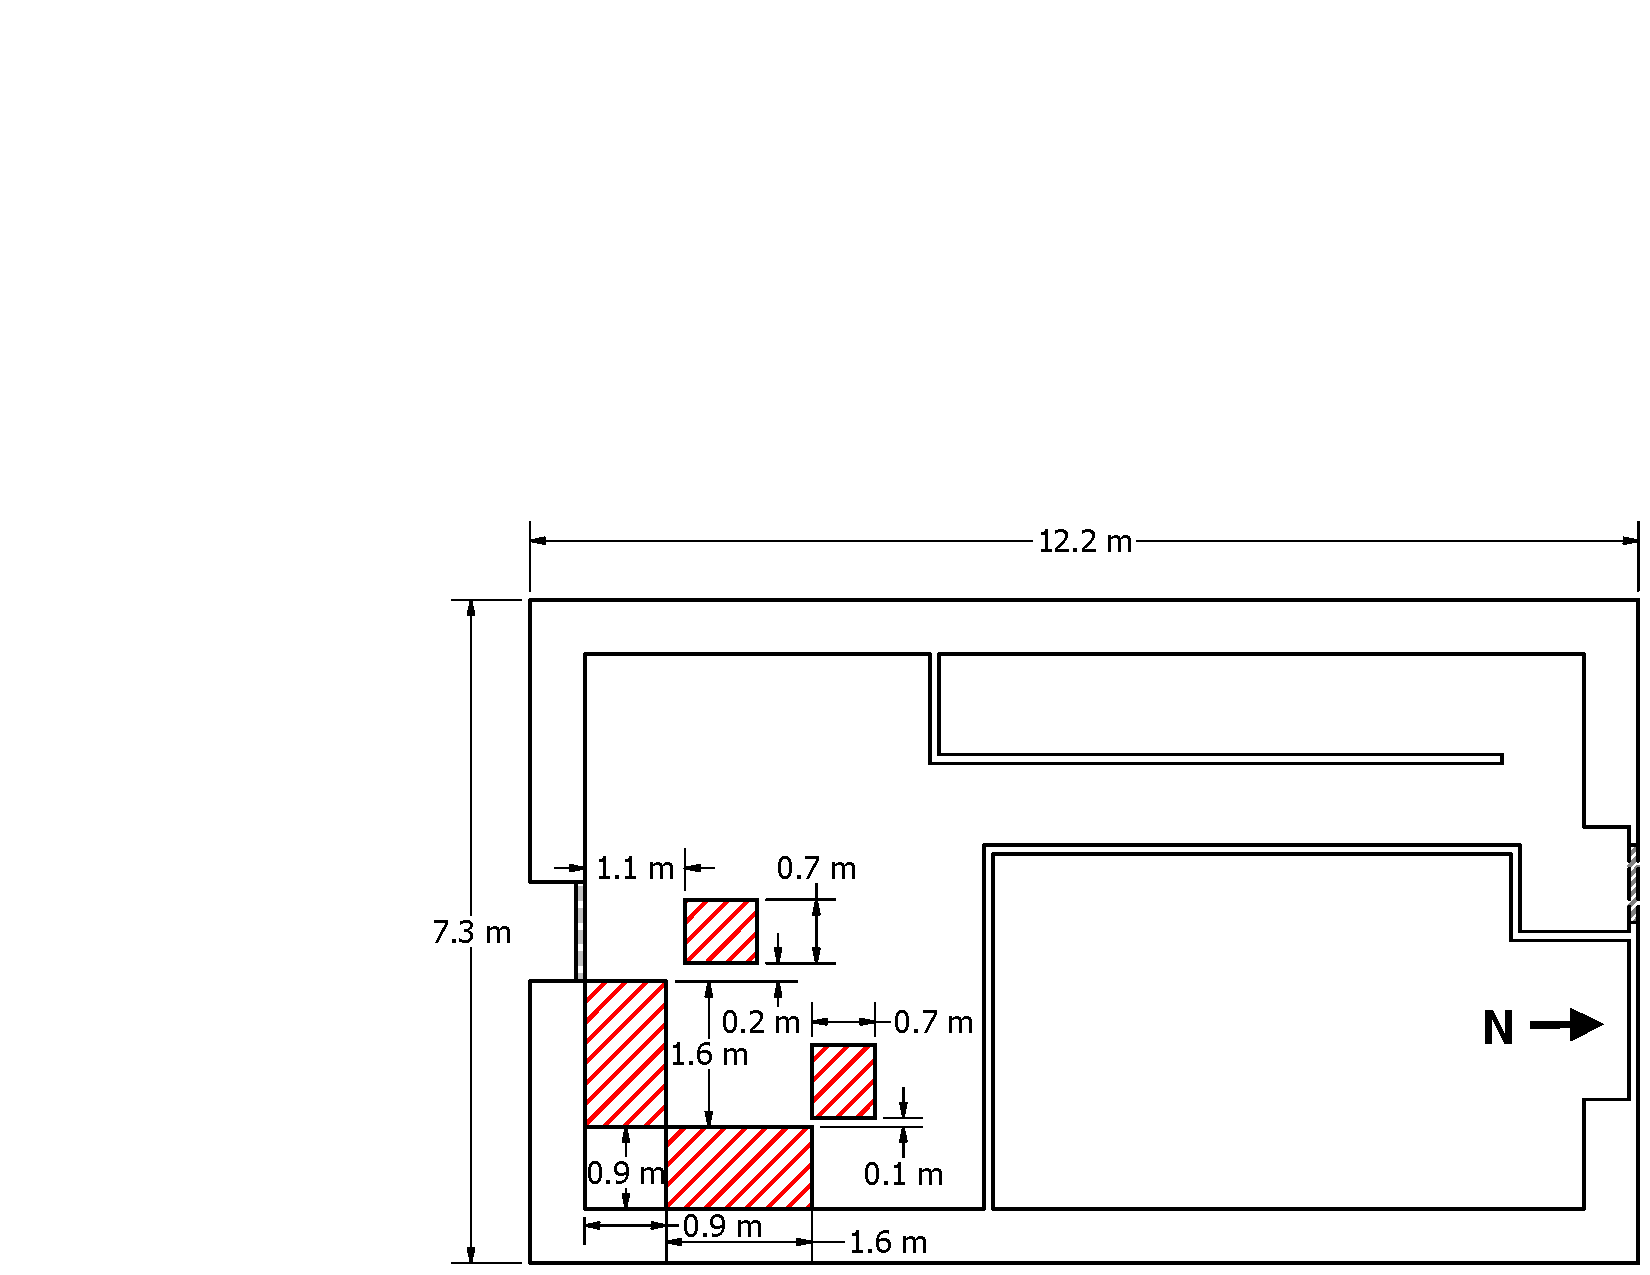
\includegraphics[width=.8\columnwidth]{../Figures/Floor_Plans/PDFs/East_Structure/DelCo_2012_East_Structure_Furniture}
	\caption{Furniture Fuel Load Dimensions in Single Story Structure.}
	\label{fig:Furniture_Fuel_Load_Dimensions}
\end{figure}

\begin{sidewaystable}[!ht]
	\centering
	\scriptsize
	\caption{Fire Suppression Fuel masses}
	\renewcommand{\tabcolsep}{1pt}
	\begin{tabular}{lllllcc}
		\toprule[1.5pt]
		Item               & Component		& Quantity		&  Material Description             			&  Dimensions (m)            	&  Mass (kg)  		& Total Mass (kg) \\
		\midrule
		2-seat Sofa        &				& 2				& 85~\% PU Foam, 15~\% PET Fiber, Wood Frame 	&  1.68 L X 0.90 D X 0.86 H  	&  72.4    			& 144.8 \\
		           	 	   & Mattress	    & 1 per sofa	& Cover: 52~\% PP, 48~\% PET,                   &  1.83 L X 1.21 W X 0.14 H     &  14.6             & \\
		           	 	   &                &               & Filling: 66~\% PET Pad, 34~\% PET Batting     &                               &                   & \\
			           	   & Cushion    	& 2 per sofa	& 85~\% PU Foam, 15~\% PET Fiber   				&  0.69 L X 0.58 D X 0.14 H  	&  2.2     			& \\
		Blue Chair         &				& 2				& 85~\% PU Foam, 15~\% PET Fiber, Wood Frame   	&  0.81 L X 0.75 D X 0.91 H  	&  17.4    			& 34.8 \\
		    			   & Cushion        & 1 per chair   & 85~\% PU Foam, 15~\% PET Fiber				&  0.51 L X 0.57 D X 0.14 H  	&  1.7    			& \\
		Blue/Green Chair   & 				& 2				& 85~\% PU Foam, 15~\% PET Fiber, Wood Frame    &  0.77 L X 0.71 D X 0.89 H  	&  16    			& 32 \\
		                   & Cushion    	& 1 per chair	& 85~\% PU Foam, 15~\% PET Fiber		        &  0.55 L X 0.53 D X 0.15 H  	&  1.6    			& \\
		Paneling           &				& 8 panels		& Medium density fiberboard                     &  2.44 L X 1.22 W X 3.2~mm H   &  9    			& 72 \\
		Carpeting          &				& 22.3 m$^2$	& 100~\% PET                  					&  3.68 L X 6.05 W  			&  32.2				& 32.2 \\
		Carpet Padding     &				& 22.3 m$^2$	& PU                       	 				    &  3.68 L X 6.05 W X 11~mm H    &  19.8			    & 19.8 \\
		                   &                &               &                                               &                               & Total Mass        & 335.6 \\
		\bottomrule[1.25pt]
	\end{tabular}
	\label{tab:Fire_Suppression_Fuel_Masses}
\end{sidewaystable}

\subsubsection*{Two Story Structure}
\label{sec:suppresion_two}

\subsubsection{Furniture Fuel Package}
\label{sec:fire_suppression_furniture_fuel_2}

The fuel load for two of the experiments consisted of three sofas with an average mass of 48.7~kg; 51.4~m$^2$ (559~ft$^2$) of carpet and padding; and approximately 38 sheets of oriented strand board (OSB) paneling with dimensions 16~mm (0.63~in) x 1.2~m (4~ft) x 2.4~m (8~ft) along the East, West, and South walls and ceiling. The three couches are aligned along the West wall and spaced 1.2~m (4~ft) apart. The specific locations can be found in the dimensioned schematic, Fig.~\ref{fig:furniture_2story}. In total, this fuel package was composed of wood, polyurethane (PU), polyester (PET),and polyprolene (PP).

\begin{figure}[!ht]
	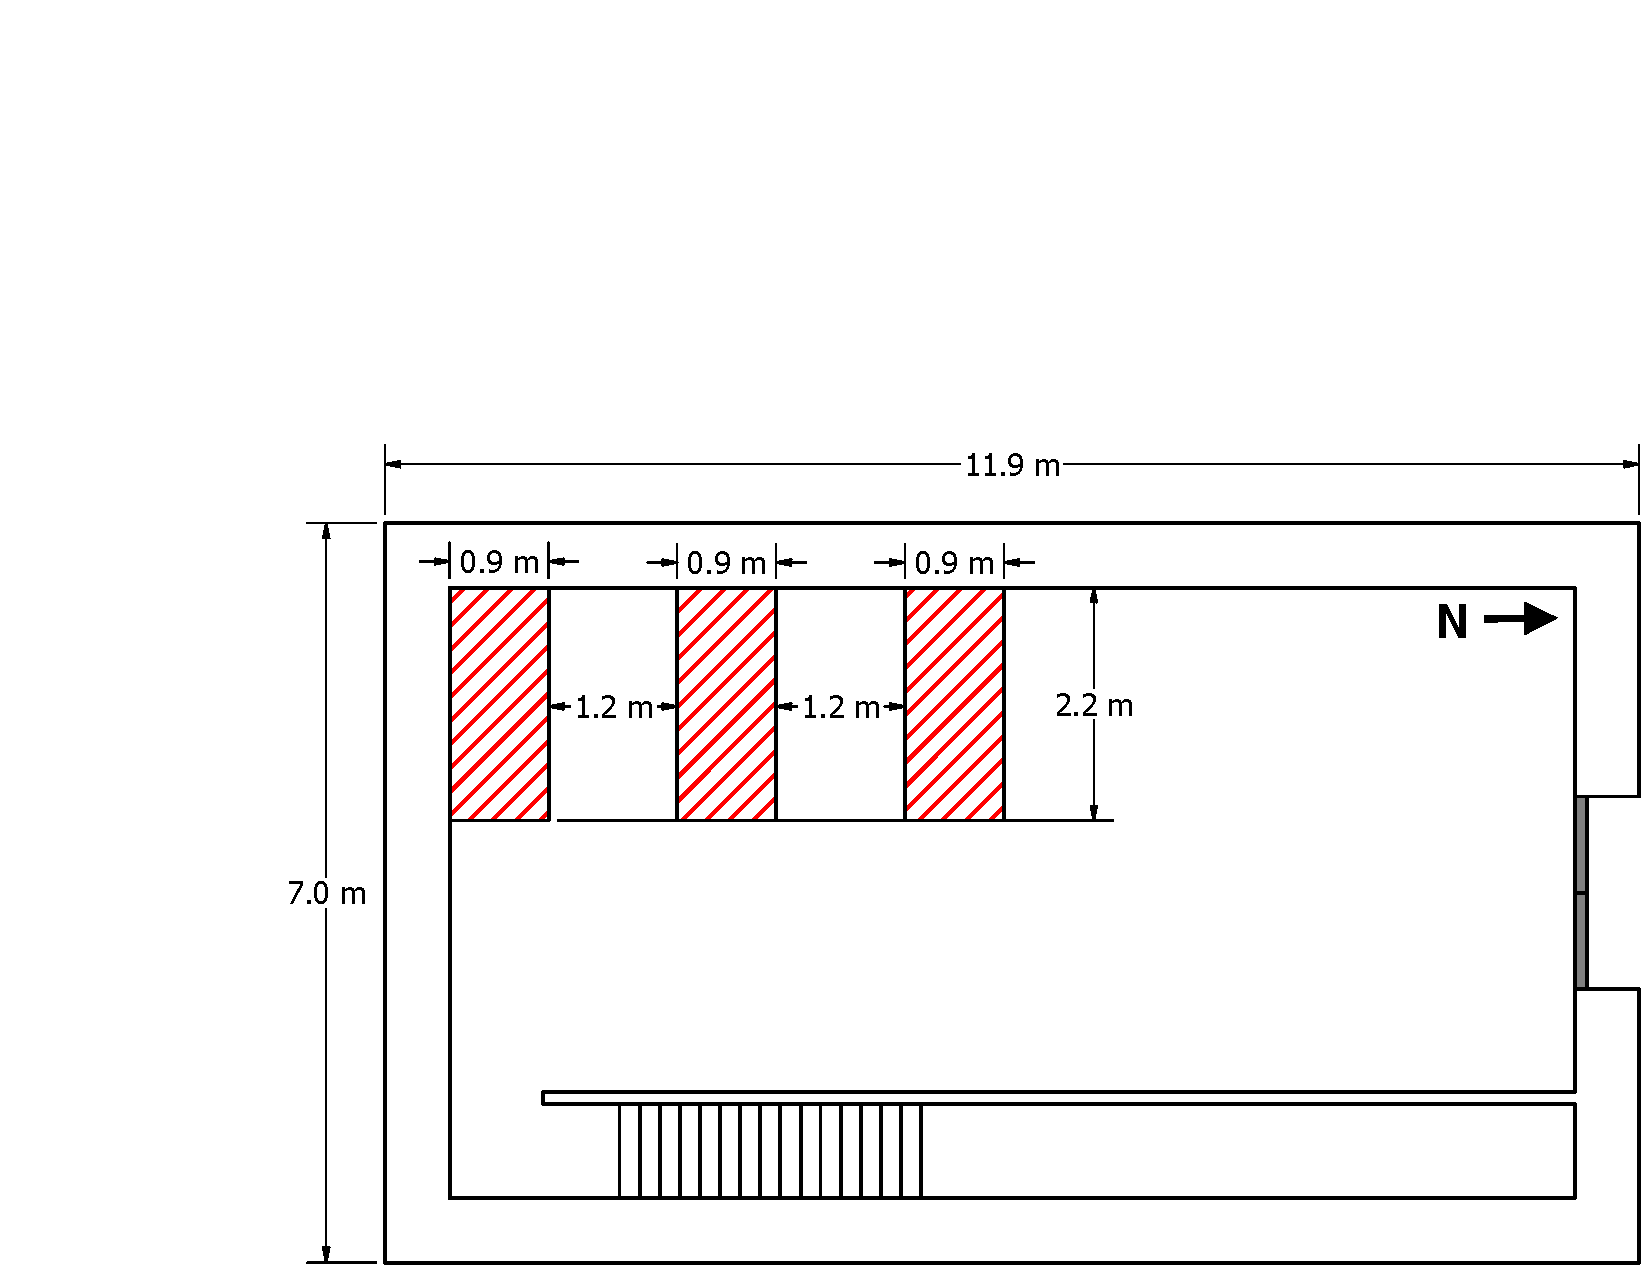
\includegraphics[width=\columnwidth]{../../DelCo_2014_2015/Drawings/PDFs/CAFS/West_Structure_1st_Floor_Furniture_Only}
	\caption{Furniture Fuel Load in First Floor of Two-Story Structure.}
	\label{fig:furniture_2story}
\end{figure}

\subsubsection{Furniture and Pallet Fuel Package}
\label{sec:fire_suppression_combo_fuel_2}

In June 2015 two stacks of pallets were added to the fuel load which consisted of three sofas, OSB lining on the ceiling and walls and the polypropylene carpeting over puf padding.  Each stack had 10 pallets.  The mass of each stack was approximately 175 kg .    When hay was added for ignition, the bales of hay averaged 12 kg.


\begin{figure}[!ht]
	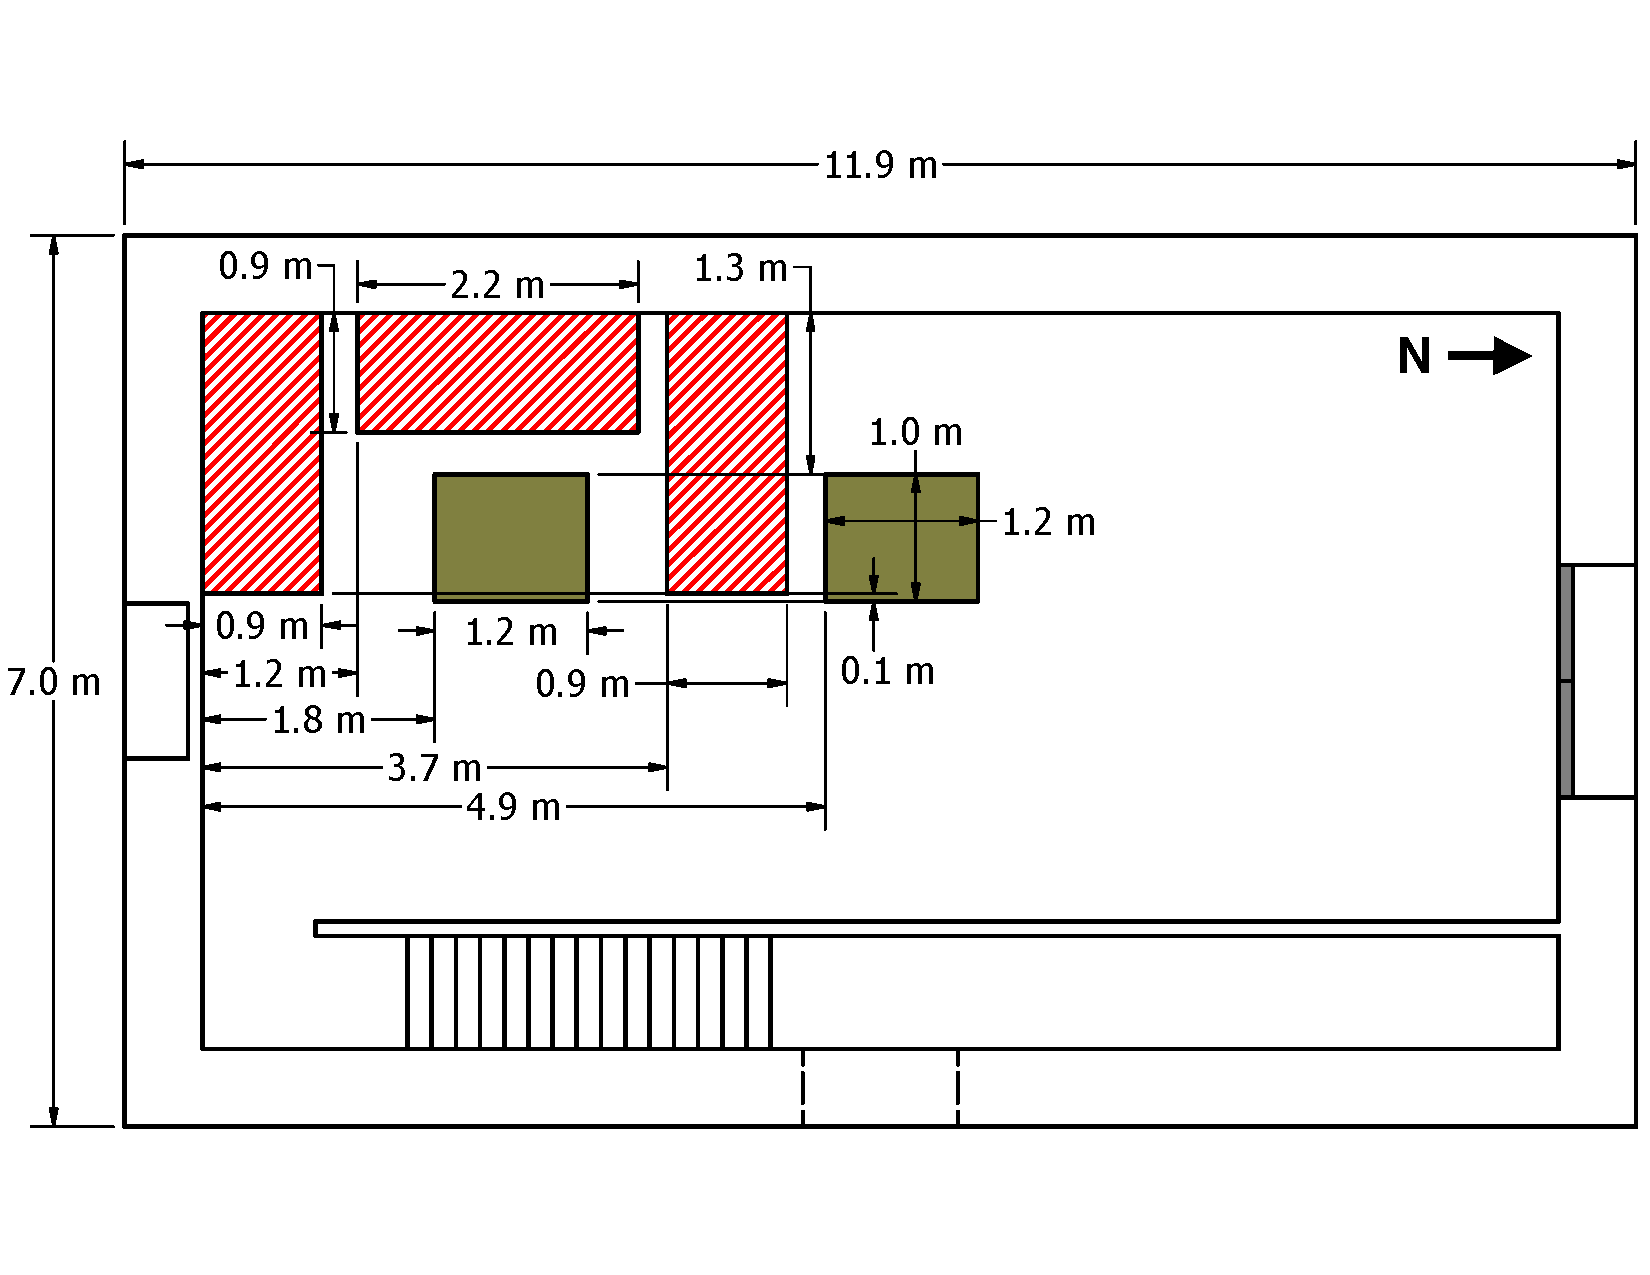
\includegraphics[width=\columnwidth]{../../DelCo_2014_2015/Drawings/PDFs/CAFS/West_Structure_1st_Floor_Furniture_Pallets}
	\caption{Furniture and Pallet Fuel Load in First Floor of Two-Story Structure.}
	\label{fig:pallet_furniture_2story}
\end{figure}



\chapter{Experiments and Results}
\label{chap:Experiments_and_Results}

\section{Spray Density}
\label{sec:Spray_Density}

Spray density experiments were conducted by placing 0.23~m$^2$ (2.5~ft$^2$) interlocking collector bins across the floor surface area of the burn rooms within each structure. The buildings were sheathed in plastic for the spray density tests to protect and preserve as much of the structure as possible before any fire suppression tests were conducted. Water flowed for a specified duration and upon completion the bins were removed from the structure. Each bin was then weighed to quantify the impact of nozzle location and spray pattern. Thirty-three spray density tests were conducted; 21 were in the burn building for the gas cooling tests and 12 were in the concrete structure for the suppression experiments. The flow rate for each test was 120~gpm for water and 120~gpm plus 60~cfm for CAFS. Tables\ref{tab:spray_density_tests} and \ref{tab:spray_density_tests2} provide an overview of each experiment. In the table, GC stands for the gas cooling experiments while SE stands for the suppression experiments. For all of the experiments, 100~ft (30~m) of 1~3/4~inch hoseline connected to a Blitz Fire monitor with a Metro 1 nozzle was used.

For the gas cooling tests, Table~\ref{tab:spray_density_tests}, the mid position had center line of the stream aimed at 2.44~m (8~ft) south of the North wall and 2.13~m (7~ft) west of the East wall in the concrete burn building. The back position had the center line of the stream aimed at 3.36~m (11~ft) south of the North wall and 2.13~m west (7~ft) of the East wall in the concrete burn building.

\begin{table}[!ht]
\footnotesize
\centering
\captionof{table}{Spray Density Test Matrix for Gas Cooling Experiments}\label{tab:spray_density_tests}
\begin{tabular}{lllll}
\toprule[1.5pt]
Test \#    &  Duration (s)  & Agent  &  Pattern            & Nozzle Position  \\
\midrule
GC1        &  15            & Water  &  Solid Stream       & Back             \\
GC2        &  23            & Water  &  Solid Stream       & Back             \\
GC3        &  15            & Water  &  Solid Stream       & Mid              \\
GC4        &  15            & Water  &  Solid Stream       & Mid              \\
GC5        &  20            & Water  &  Solid Stream       & Mid              \\
GC6        &  21            & Water  &  30$^{\circ}$ Fog   & Mid              \\
GC7        &  20            & Water  &  30$^{\circ}$ Fog   & Mid              \\
GC8        &  22            & Water  &  30$^{\circ}$ Fog   & Back             \\
GC9        &  24            & Water  &  30$^{\circ}$ Fog   & Back             \\
GC10       &  20            & Water  &  Solid 7/8~in Slug  & Back             \\
GC11       &  22            & Water  &  Solid 7/8~in Slug  & Back             \\
GC12       &  15            & CAFS    &  Smooth Bore 7/8~in & Back             \\
GC13       &  10            & CAFS    &  Smooth Bore 7/8~in & Mid              \\
GC14       &  15            & CAFS    &  Smooth Bore 7/8~in & Back             \\
GC15       &  20            & CAFS    &  Smooth Bore 7/8~in & Mid              \\
GC16       &  15            & CAFS    &  30$^{\circ}$ Fog   & Mid              \\
GC17       &  20            & CAFS    &  Solid Stream       & Mid             \\
GC18       &  10            & CAFS    &  Solid Stream       & Mid             \\
GC19       &  15            & CAFS    &  30$^{\circ}$ Fog   & Back             \\
GC20       &  15            & CAFS    &  30$^{\circ}$ Fog   & Back             \\
GC21       &  15            & CAFS    &  Solid Stream       & Back             \\

\bottomrule[1.25pt]
\end{tabular}\par
\end{table}
For the fire suppression spray density experiments, Table~\ref{tab:spray_density_tests2}, the hallway position had the center of the stream aimed at the ceiling of the burn room, 2.14~m (7~ft) north of the South wall and 1.53~m (5~ft) east of the West wall. The fire room position had the center of the stream aimed at the ceiling of the burn room, 2.14~m (7~ft) north of the South wall and 3.05~m (10~ft) west of the East wall.

\begin{table}[!ht]
\footnotesize
\centering
\captionof{table}{Spray Density Test Matrix for Fire Suppression Experiments}\label{tab:spray_density_tests2}
\begin{tabular}{lllll}
\toprule[1.5pt]
Test \#    & Duration (s)  & Agent  &  Pattern            & Nozzle Location  \\
\midrule
SE1        & 7             & Water  &  Solid Stream       &    Fire Room          \\
SE2        & 18            & Water  &  Solid Stream       &    Fire Room          \\
SE3        & 19            & Water  &  Solid Stream       &    Fire Room          \\
SE4        & 21            & Water  &  Solid Stream       &    Fire Room          \\
SE5        & 22            & Water  &  30$^{\circ}$ Fog   &    Fire Room          \\
SE6        & 19            & Water  &  30$^{\circ}$ Fog   &    Fire Room          \\
SE7        & 16            & Water  &  Solid 7/8~in Slug  &    Fire Room          \\
SE8        & 17            & Water  &  Solid 7/8~in Slug  &    Hallway            \\
SE9        & 15            & Water  &  30$^{\circ}$ Fog   &    Hallway            \\
SE10       & 16            & Water  &  30$^{\circ}$ Fog   &    Hallway            \\
SE11       & 16            & Water  &  Solid Stream       &    Hallway            \\
SE12       & 16            & Water  &  Solid Stream       &    Hallway            \\
\bottomrule[1.25pt]
\end{tabular}\par
\end{table}

\clearpage

After weighing each of the bins the mass of water (kg) in each bin was plotted by position to visualize the spray distribution. Figure~\ref{fig:Burn_Building_Test_1} shows that with a straight stream in the back position, the majority of the water accumulated along the North and East walls of the gas cooling room within the burn building (cf. Fig.~\ref{fig:Delaware_County,_PA_Burn_Building_Layout}). Figure~\ref{fig:Burn_Building_Test_7} shows difference a fog stream as the distribution of water is far more dispersed around the gas cooling room. The remainder of the burn building spray density figures are included in Appnedix~\ref{app:spray_density}.

\begin{figure}[!ht]
	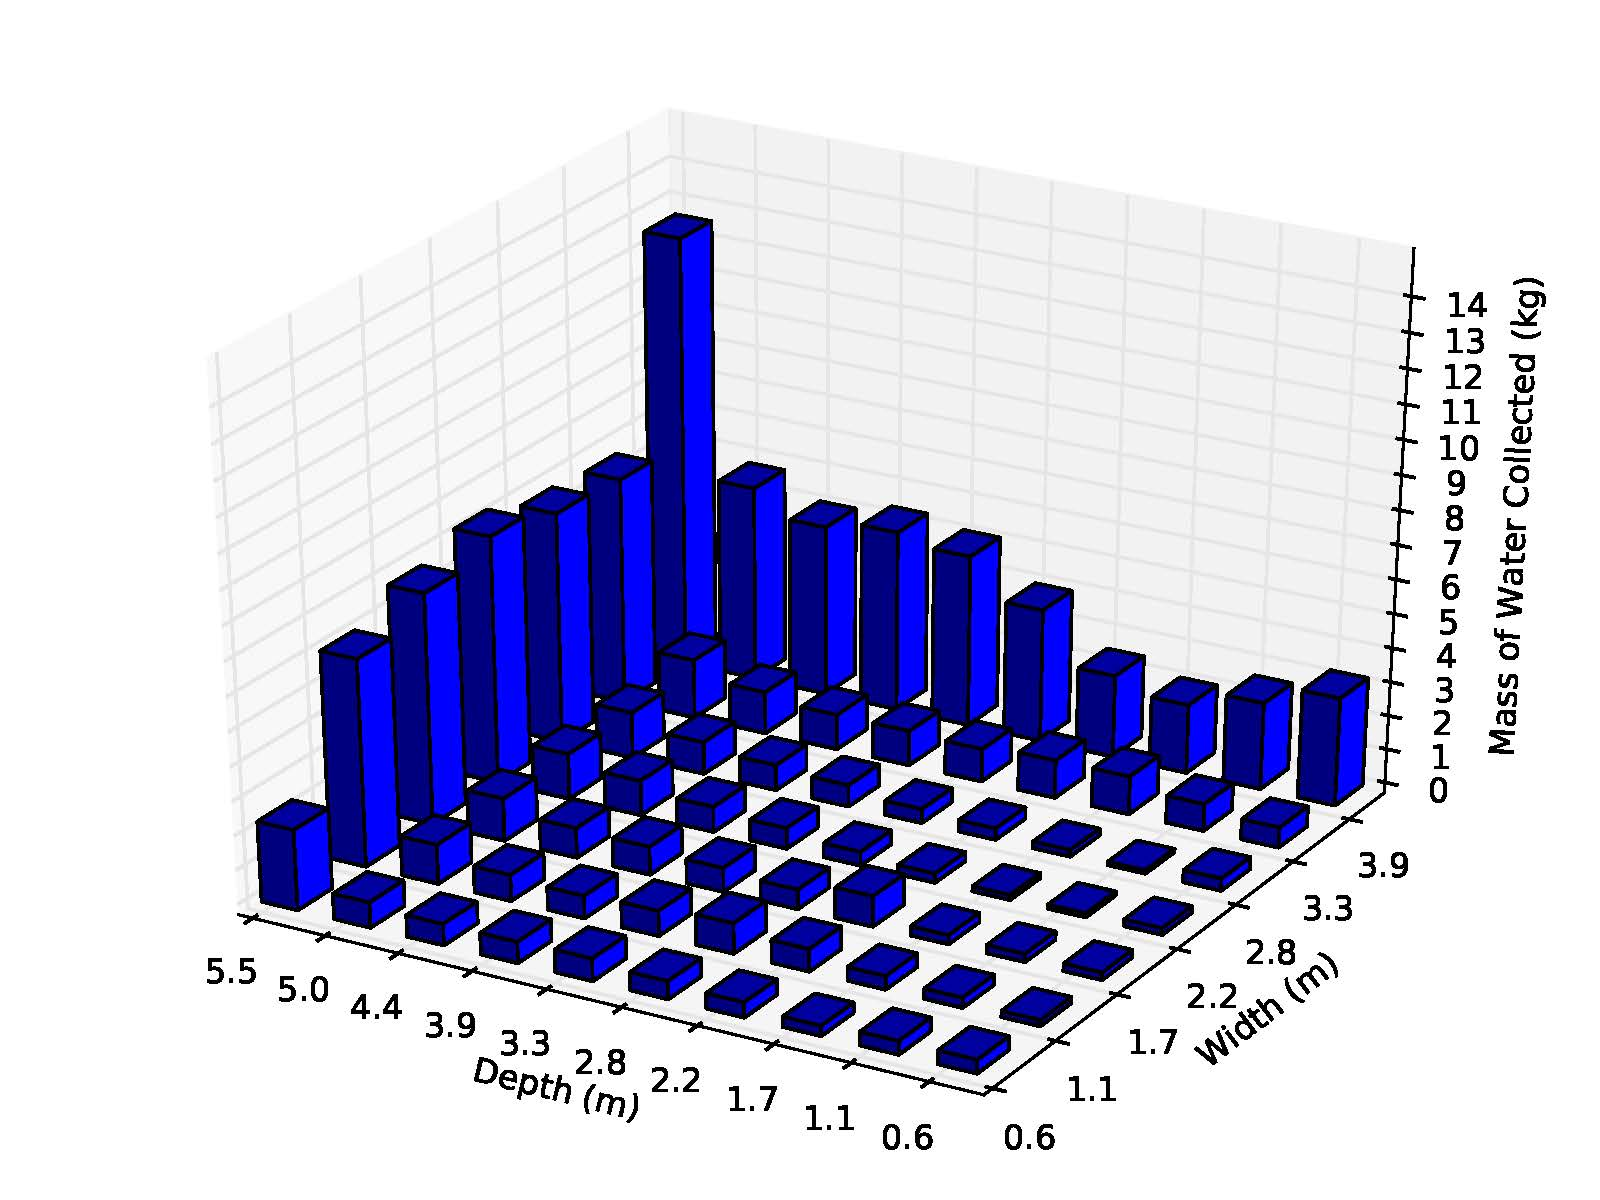
\includegraphics[width=4in]{../Figures/Bars/BB1}
	\caption{Gas Cooling Spray Density Test 1}
	\label{fig:Burn_Building_Test_1}
\end{figure}

\begin{figure}[!ht]
	\includegraphics[width=4in]{../Figures/Bars/BB7}
	\caption{Gas Cooling Spray Density Test 7}
	\label{fig:Burn_Building_Test_7}
\end{figure}


\clearpage

\section{Gas Cooling}
\label{sec:Gas_Cooling}

The 88 gas cooling events were completed as part of 9 separate tests in the burn building. During each test, the fire was ignited and then developed until the temperature 1.83~m (6~ft) below the ceiling in the gas cooling room reached or exceeded 250~$^{\circ}$C (482~$^{\circ}$F). Once this criteria was met, gas cooling began. Figure~\ref{fig:gas_cooling_exp4} shows 19 cooling events at one thermocouple array during a continuous test.

\begin{figure}[ht!]
	\includegraphics[width=\columnwidth]{../Figures/Gas_Cooling/GCSeries4_TC_A3}
	\caption{Time Series of Multiple Gas Cooling Events From a 1 of 9 Tests}
	\label{fig:gas_cooling_exp4}
\end{figure}

There were three thermocouple arrays in the gas cooling room (adjacent to the burn room in Fig.~\ref{fig:Gas_Cooling_Instrumentation_Dimensions}). Figures~\ref{fig:gas_cooling_sub1} and \ref{fig:gas_cooling_sub5} show the variation of the impact of the suppression stream on cooling location for three consecutive water and CAFS tests, respectively. For both sets a solid 7/8 in nozzle in the middle position was used. The data shows that thermocouples in the plot in the upper right of both figures has more significant temperature drops than the other two arrays; this is likely a result of that thermocouple array being directly ``hit'' by the suppression stream.

\begin{figure}[ht!]
	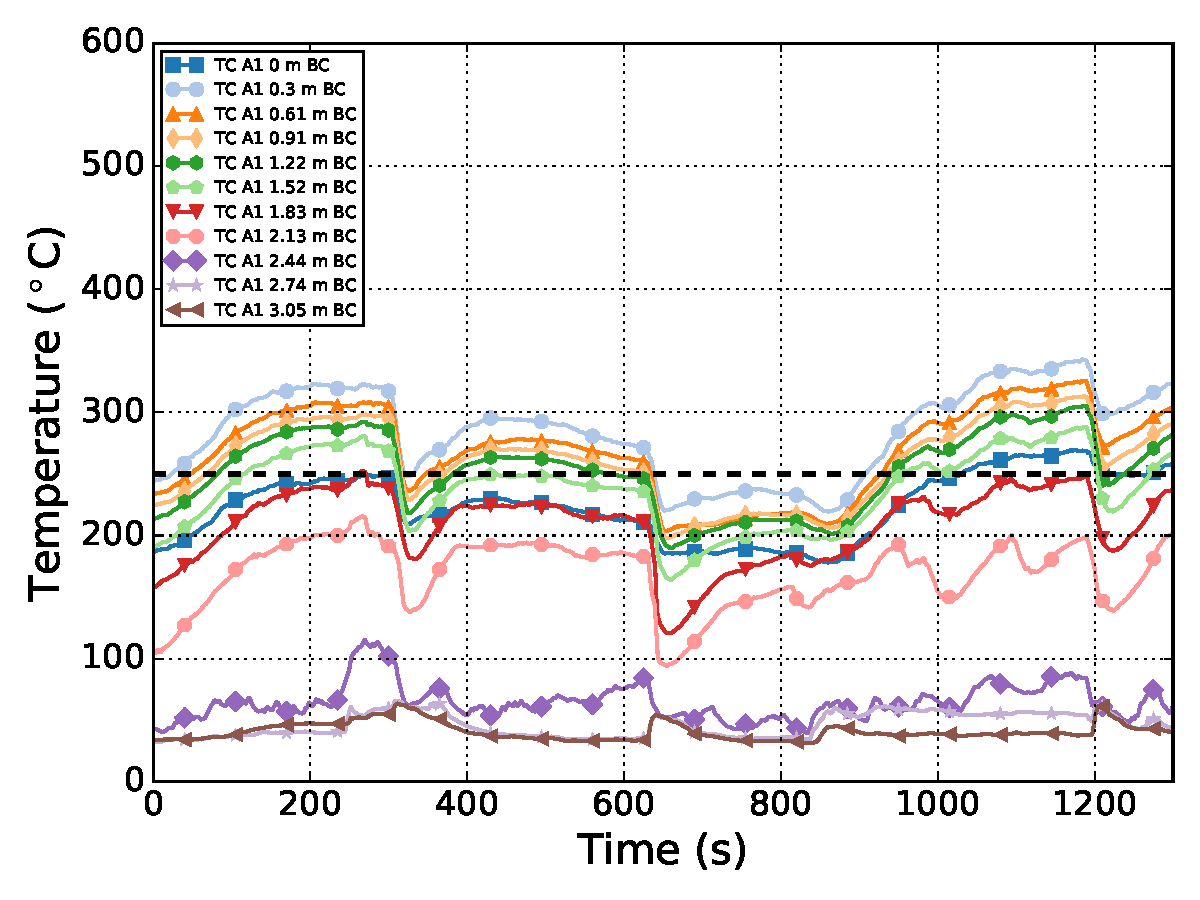
\includegraphics[width=.5\columnwidth]{../Figures/Gas_Cooling/GCSeries12_TC_A1}
	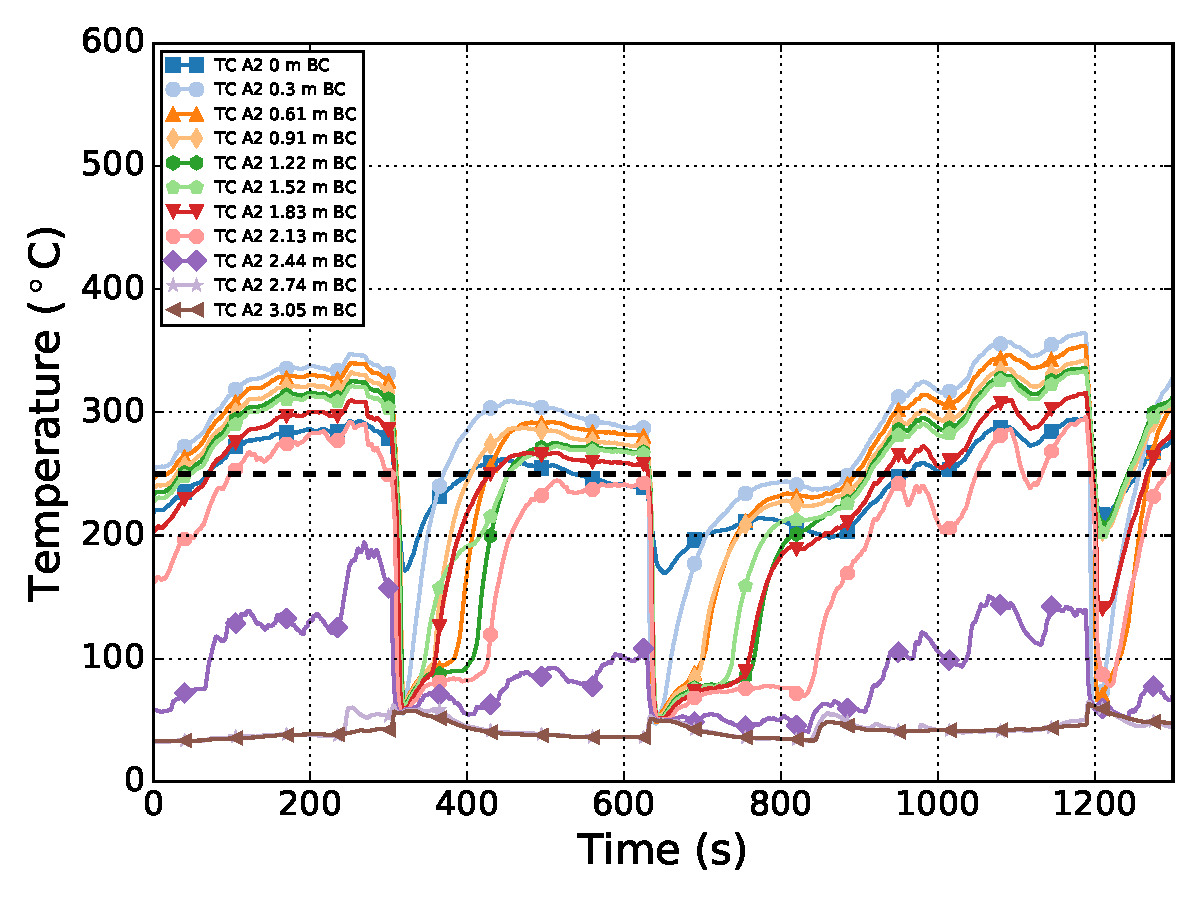
\includegraphics[width=.5\columnwidth]{../Figures/Gas_Cooling/GCSeries12_TC_A2}
	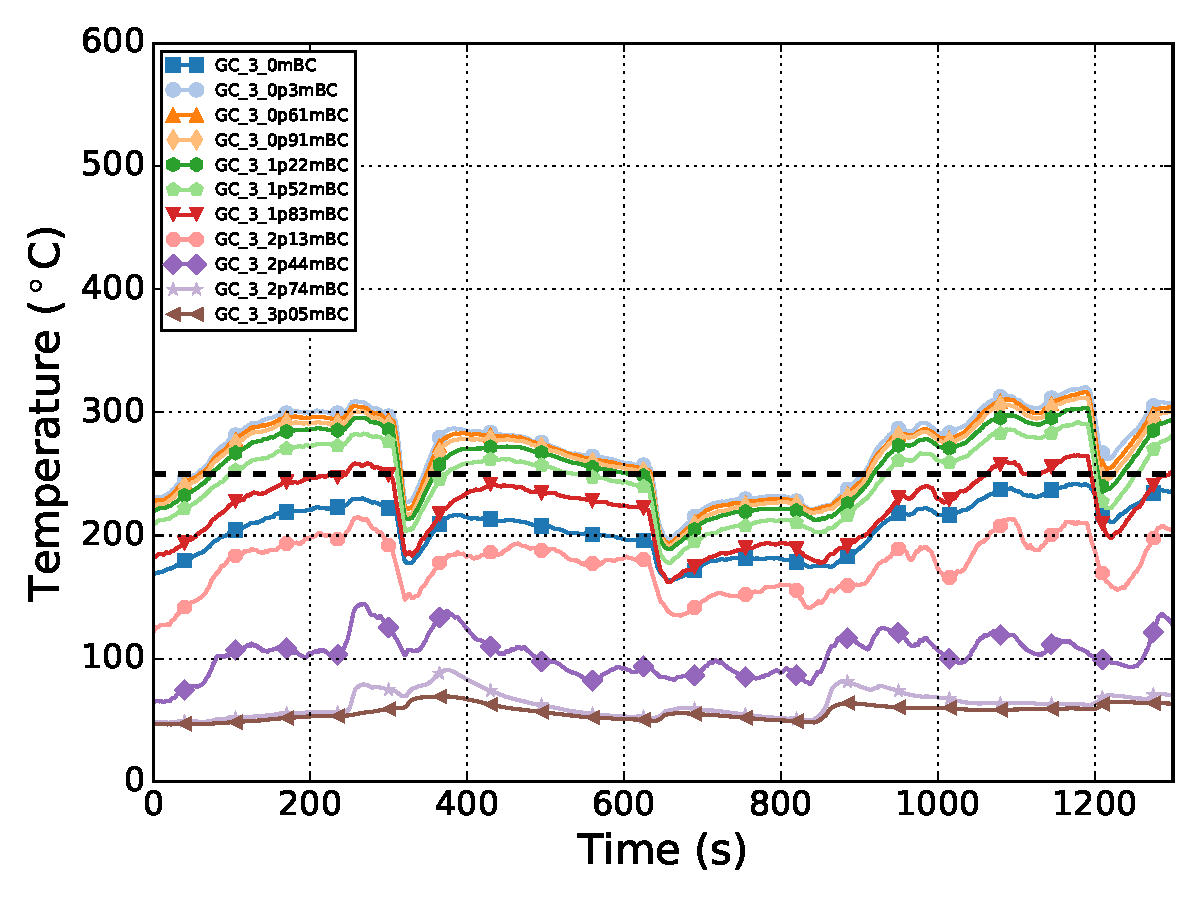
\includegraphics[width=.5\columnwidth]{../Figures/Gas_Cooling/GCSeries12_TC_A3}
	\caption{Time Series of Thermocouple Data from 3 Arrays in Gas Cooling Room with Water as Suppression Agent}
	\label{fig:gas_cooling_sub1}
\end{figure}

\begin{figure}[ht!]
	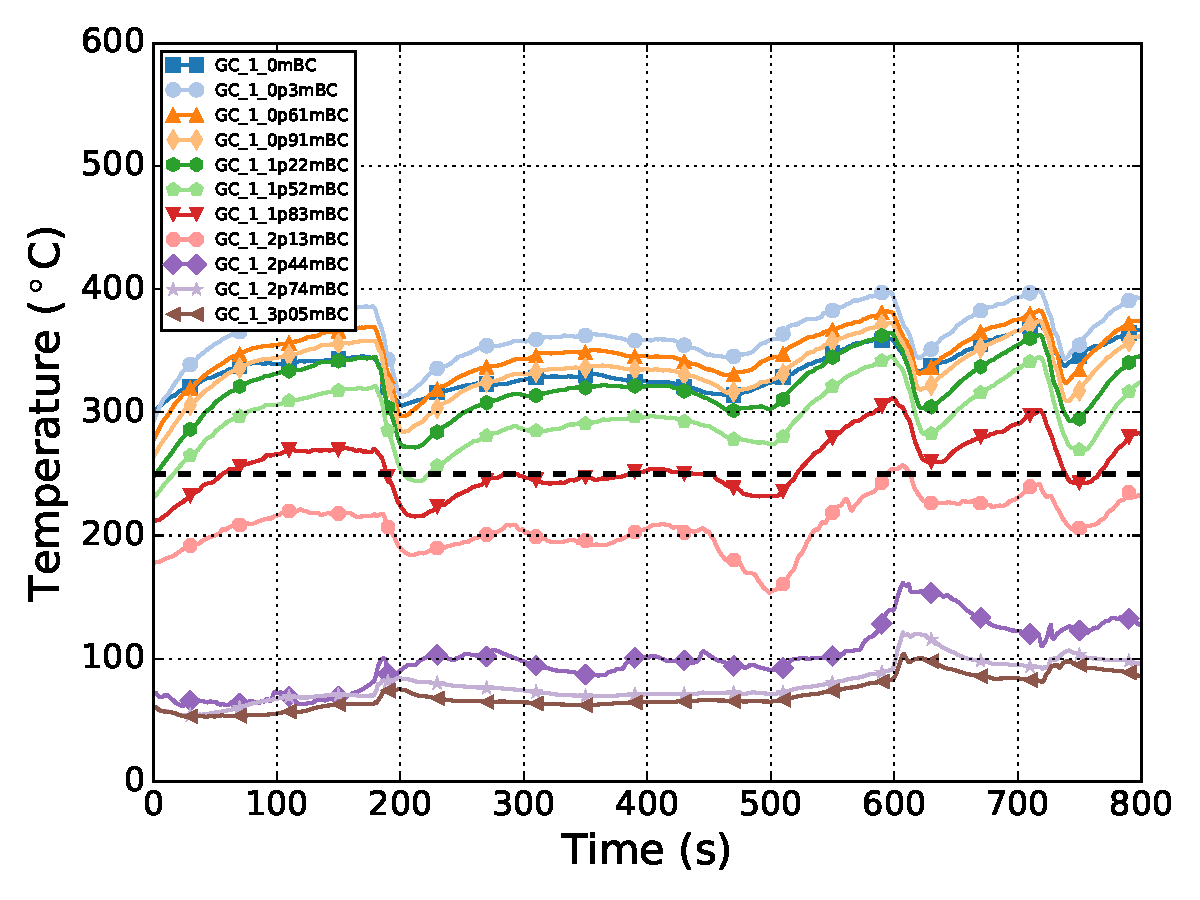
\includegraphics[width=.5\columnwidth]{../Figures/Gas_Cooling/GCSeries52_TC_A1}
	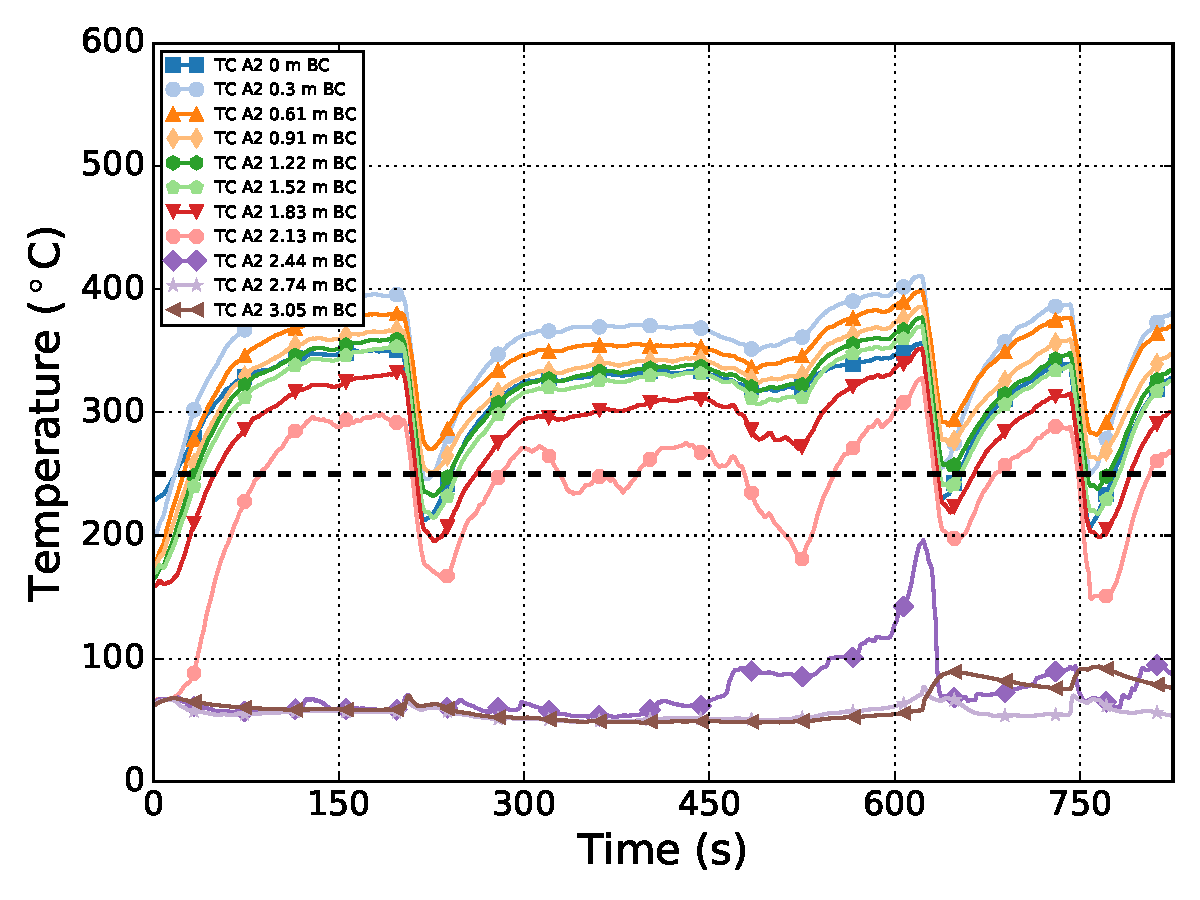
\includegraphics[width=.5\columnwidth]{../Figures/Gas_Cooling/GCSeries52_TC_A2}
	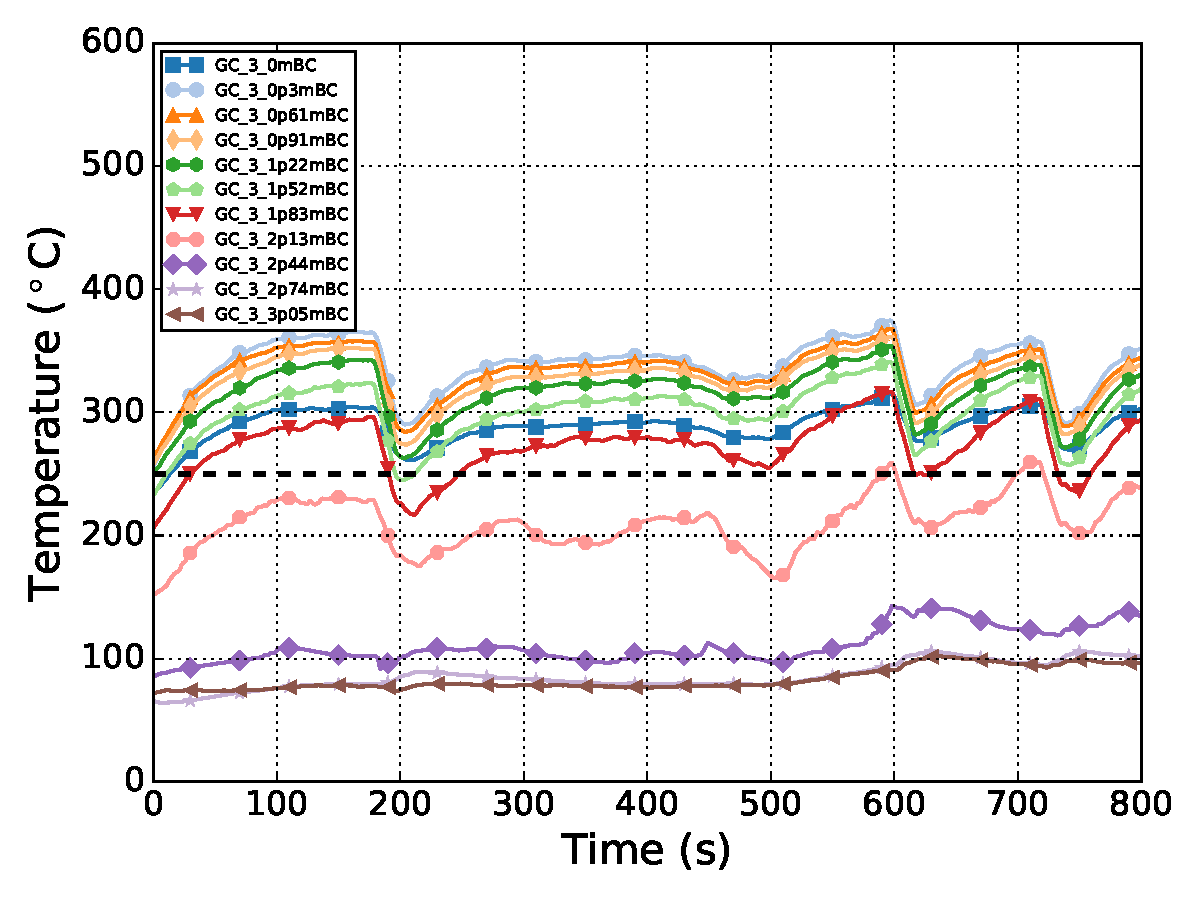
\includegraphics[width=.5\columnwidth]{../Figures/Gas_Cooling/GCSeries52_TC_A3}
	\caption{Time Series of Thermocouple Data from 3 Arrays in Gas Cooling Room with CAFS as Suppression Agent}
	\label{fig:gas_cooling_sub5}
\end{figure}

\clearpage

To better quantify the effectiveness of the suppression agents (CAFS, water), the maximum temperature differences associated with each gas cooling event for each agent from the three thermocouple trees were analyzed. Figure~\ref{fig:combined_all} compares the temperature differences at each thermocouple position (via a scatterplot) for the 30 replicate tests, 15 water and 15 CAFS, for all streams aimed at all positions.

\begin{figure}[!ht]
	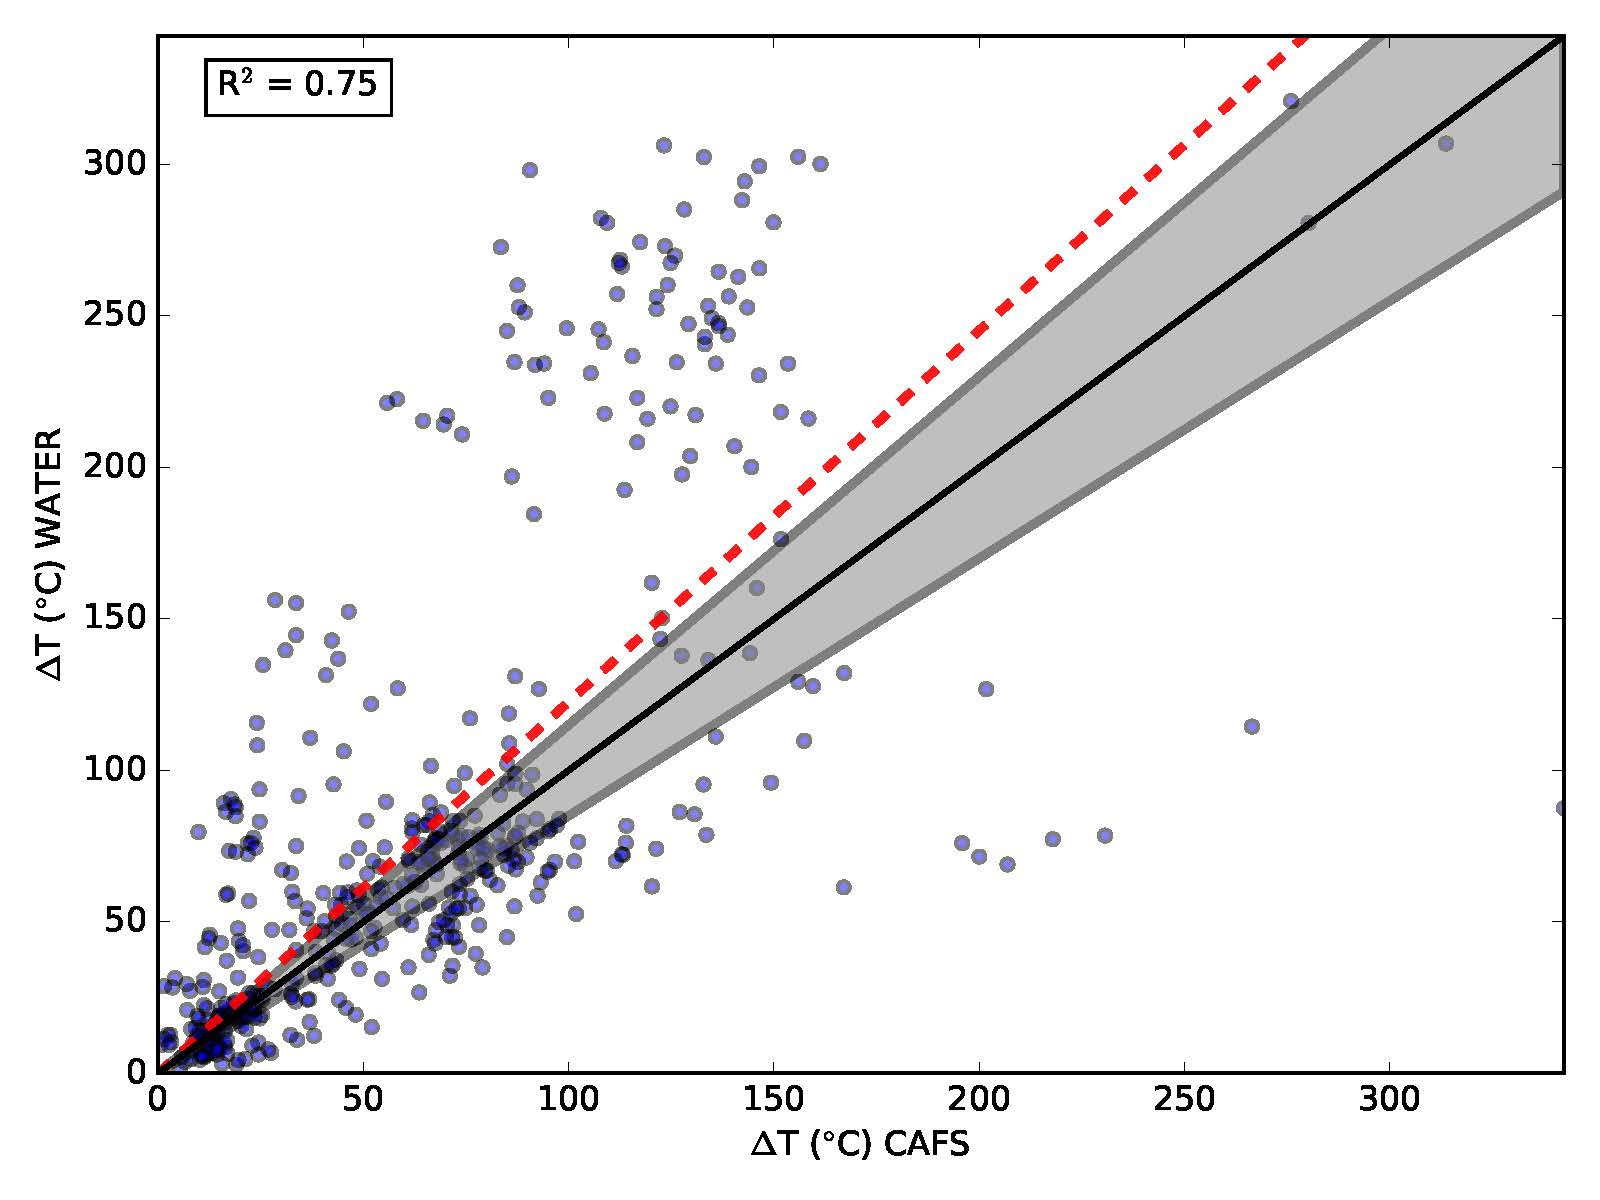
\includegraphics[width=.8\columnwidth]{../Figures/Gas_Cooling/Combined_scatter}
	\caption{CAFS vs Water Gas Cooling Comparison for All Replicate Tests}
	\label{fig:combined_all}
\end{figure}

The circles in Fig.~\ref{fig:combined_all} are the maximum temperature differences for each measurement point for all the replicate cooling events. If water and CAFS have the exact same temperature differences, all of the points would fall along solid black line in the figure. Circles that vary from that line represent measurements where either water (above) or CAFS (below) cooled more significantly than the other agent. The gray area surrounding the solid black line, represents measurement uncertainty (\ref{subsec:Uncertainty}). For data that fall within this area, there is an inability to determine which agent was more or less effective than the other. The red dashed line is the line the describes the data by minimizing the differences between the two suppression agents through a linear approximation of the data. Since this line falls above the gray area for the comparison, water shows a better ability to cool gas under the same test criteria as CAFS.

The data can be separated to examine the impact of nozzle position (back or middle position) on the ability to cool gases for each of the suppression agents. Figures~\ref{fig:CAFS_Water_mid} and \ref{fig:CAFS_Water_full} show the cooling comparison for 12 replicates in the back position and 3 replicates in the middle position respectively.

\begin{figure}[!ht]
	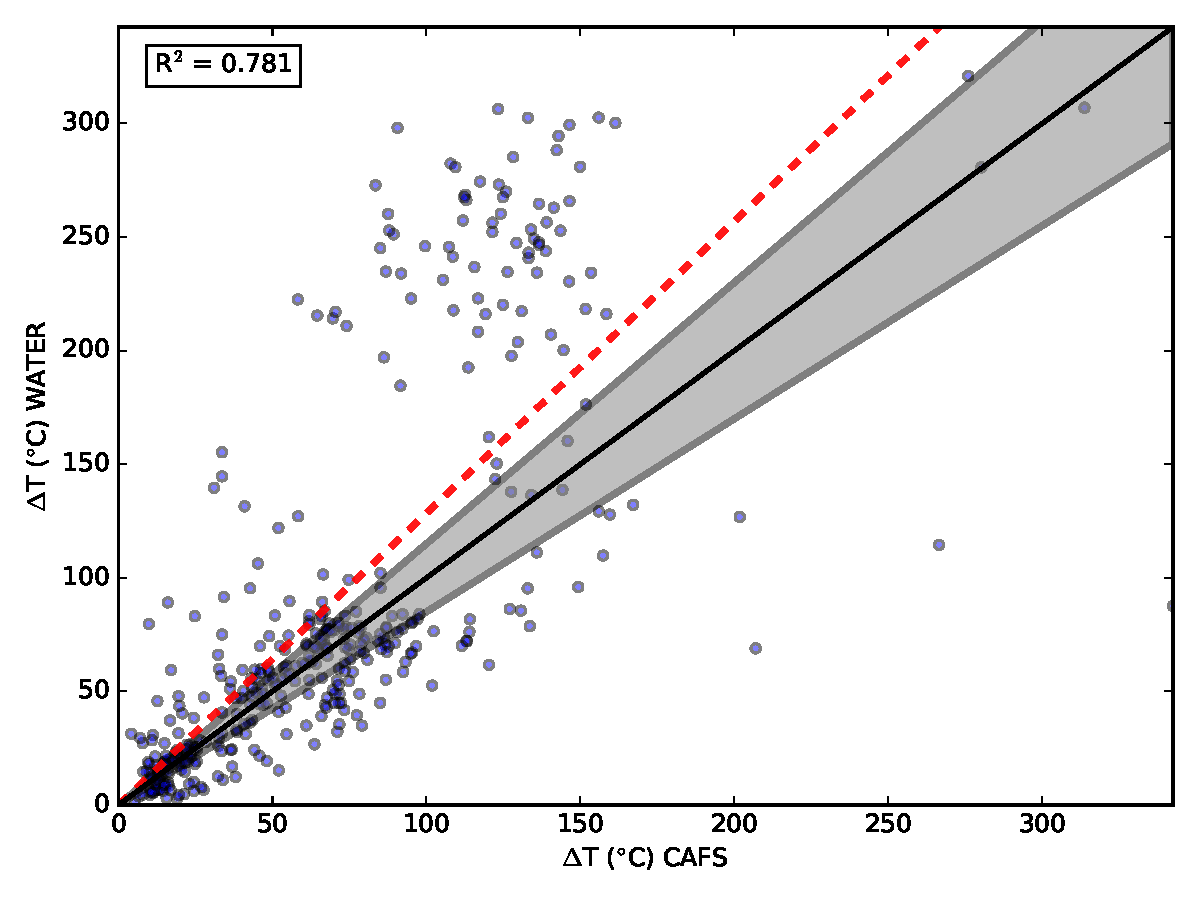
\includegraphics[width=.8\columnwidth]{../Figures/Gas_Cooling/Combined_mid_scatter}
	\caption{CAFS vs Water Gas Cooling Comparison for Middle Position}
	\label{fig:CAFS_Water_mid}
\end{figure}

\begin{figure}[!ht]
	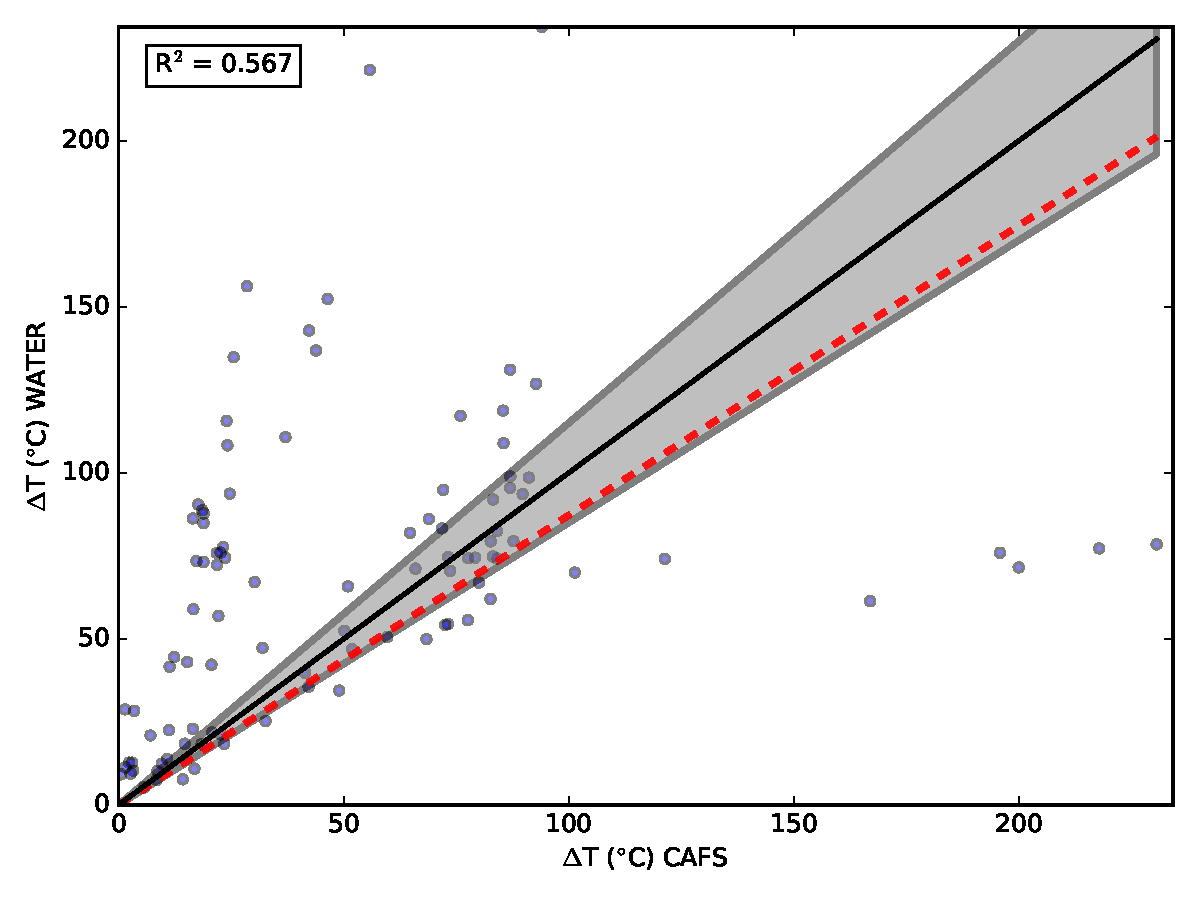
\includegraphics[width=.8\columnwidth]{../Figures/Gas_Cooling/Combined_fullback_scatter}
	\caption{CAFS vs Water Gas Cooling Comparison for Back Position}
	\label{fig:CAFS_Water_full}
\end{figure}

For the 12 middle position replicate comparisons (Fig.~\ref{fig:CAFS_Water_mid}), the results (via the dashed red line) show that water has a slight advantage in gas cooling relative to CAFS. At the back position (Fig.~\ref{fig:CAFS_Water_full}), for the 3 replicate comparison, the least squared error line falls within the experimental uncertainty. This indicates an inability to distinguish between the two suppression agents with statistical confidence. The data can be further divided to analyze the impact of the nozzle type on comparison between water and CAFS. Figures~\ref{fig:CAFS_Water_78_mid} and \ref{fig:CAFS_Water_SS_mid} show the results for 7 replicate comparisons of a 7/8~in. solid stream and 5 replicate comparisons of a straight stream respectively; both aimed at the middle position. 

\begin{figure}[!ht]
	\includegraphics[width=.8\columnwidth]{../Figures/Gas_Cooling/7_8_Solid_mid_scatter}
	\caption{CAFS vs Water Gas Cooling Comparison for 7/8~in. Solid Stream Mid Position}
	\label{fig:CAFS_Water_78_mid}
\end{figure}

\begin{figure}[!ht]
	\includegraphics[width=.8\columnwidth]{../Figures/Gas_Cooling/SS_mid_scatter}
	\caption{CAFS vs Water Gas Cooling Comparison for Straight Stream Mid Position}
	\label{fig:CAFS_Water_SS_mid}
\end{figure}

The 7 replicate tests comparing water and CAFS from a 7/8~in. solid stream nozzle aimed at the middle position show a large bias towards water. For the 5 replicate tests with a straight stream nozzle, the least squared error line fit through the data falls along the edge of the measurement uncertainty bounds on the water side of comparison. 

The back position can also be decomposed to compare stream type. Figure~\ref{fig:CAFS_Water_SS_back} shows a single comparison between water and CAFS for a straight stream in the back position while Fig.~\ref{fig:CAFS_Water_Fog_back} shows a 2 replicate comparison between water and CAFS for a 30$^{\circ}$ Fog in the back position.

\begin{figure}[!ht]
	\includegraphics[width=.8\columnwidth]{../Figures/Gas_Cooling/SS_full_back_scatter}
	\caption{CAFS vs Water Gas Cooling Comparison for Straight Stream Back Position}
	\label{fig:CAFS_Water_SS_back}
\end{figure}

\begin{figure}[!ht]
	\includegraphics[width=.8\columnwidth]{../Figures/Gas_Cooling/30_Fog_full_back_scatter}
	\caption{CAFS vs Water Gas Cooling Comparison for 30$^{\circ}$ Fog Back Position}
	\label{fig:CAFS_Water_Fog_back}
\end{figure}

For the straight stream comparison (Fig.~\ref{fig:CAFS_Water_SS_back}), there is an inability to distinguish between the suppression agents with statistical confidence. The 30$^{\circ}$ Fog replicate comparison (Fig.~\ref{fig:CAFS_Water_Fog_back}) shows that CAFS has better cooling potential compared to water.

\clearpage

\section{Fire Suppression}
\label{sec:Fire_Suppression}

\subsubsection*{Single Story Structure}
\label{sec:fire_supp_single}

There were 14 suppression tests conducted in the single story purpose-built concrete structure. Four of the tests used a wood pallet fuel load (Section~\ref{sec:fire_suppression_pallet_fuel}) and the remaining tests used a fuel load comprised of typical household furnishings that included wooden wall paneling, two sofas, two overstuffed chairs, carpet, and padding (Section~\ref{sec:fire_suppression_furniture_fuel}). Ignition occurred in the rear of the single story structures and the available ventilation was through the front doorway and for several tests a rear window was opened to provide additional ventilation (see Table~\ref{tab:Test_Descriptions}). The fires were intended to replicate room and contents fires typically seen within residential structures. Hose lines were pre-deployed with fixed nozzles set in two locations: one in the hallway on the approach to the burn room (hallway nozzle) and one just inside the burn room to the right side of the hallway (room nozzle). Each nozzle flowed 15~s of water or compressed air foam depending on the test. The hallway nozzle was intended to simulate a crew advancing into a structure towards the burn room. Suppression from this location would be in the form of gas cooling as the stream was not aimed at the seat of the fire (indirect interior attack). The room nozzle was intended to simulate a crew which had advanced into a structure, entered the fire room, positioned just to the side of the entry door, and began suppression on the seat of the fire (direct interior attack). Table~\ref{tab:Test_Descriptions} provides an overview of the suppression tests conducted.

\begin{table}[!ht]
\centering
\caption{Fire Suppression Test Descriptions}\label{tab:Test_Descriptions}
\begin{tabular}{clllll}
\toprule[1.5pt]
Test $\#$  & Name	& Stream			& Flow Rate		& Fuel           & Ventilation     \\
\midrule
 1 & CAFS~1   &  30$^{\circ}$ Fog   &  120~gpm/60~cfm   & Furniture      & Door            \\
 2 & Water~1  &  30$^{\circ}$ Fog  	&  120~gpm    		& Furniture      & Door            \\
 3 & CAFS~2   &  7/8'' Smooth Bore  &  120~gpm/60~cfm   & Furniture      & Door            \\
 4 & Water~2  &  7/8'' Smooth Bore  &  120~gpm    		& Furniture      & Door            \\
 5 & Water~3  &  30$^{\circ}$ Fog  	&  120~gpm    		& Furniture      & Door + Window   \\
 6 & CAFS~3   &  30$^{\circ}$ Fog   &  120~gpm/60~cfm   & Furniture      & Door + Window   \\
 7 & Water~4  &  30$^{\circ}$ Fog  	&  120~gpm    		& Furniture      & Door + Window   \\
 8 & CAFS~4   &  30$^{\circ}$ Fog   &  120~gpm/60~cfm   & Furniture      & Door + Window   \\
 9 & Attic~1  &  Straight Stream  	&  120~gpm    		& Furniture      & Door            \\
10 & Attic~2  &  Straight Stream  	&  120~gpm/60~cfm   & Furniture      & Door            \\
11 & Water~5  &  30$^{\circ}$ Fog  	&  120~gpm   		& Wood           & Door + Window   \\
12 & CAFS~5   &  30$^{\circ}$ Fog   &  120~gpm/60~cfm   & Wood           & Door + Window   \\
13 & Water~6  &  30$^{\circ}$ Fog  	&  120~gpm    		& Wood           & Door + Window   \\
14 & CAFS~6   &  30$^{\circ}$ Fog   &  120~gpm/60~cfm   & Wood           & Door + Window   \\
\bottomrule[1.25pt]
\end{tabular}\par
\end{table}

Table~\ref{tab:Test_Results} provides the impact of the two nozzle applications for the water and CAFS tests. The table provides change in temperature 0.3~m (1~ft) below the ceiling and 0.3~m (1~ft) above the floor as well as change in heat flux 0.15~m (6~in) above the floor at the measurement location closest to the fire. These values reported in the table are immediately before and after the 15~s application period to assess the application agent, stream, and location on interior conditions.

\begin{table}[!ht]
\centering
\caption{Fire Suppression Results}\label{tab:Test_Results}
\begin{tabular}{lccc}
\toprule[1.5pt]
                 & \multicolumn{2}{c}{Temperature Change}                                    & Heat Flux Change \\
Test 	         & 0.3~m (1~ft) Below Ceiling          & 0.3~m (1~ft) Above Floor	         & 0.15~m (6~in) Above Floor \\
\midrule
CAFS~1 Hallway   & 770~$^{\circ}$C - 190~$^{\circ}$C   & 680~$^{\circ}$C - 170~$^{\circ}$C   & 70~kW/m$^2$ - 20~kW/m$^2$  \\
CAFS~1 Room      & 250~$^{\circ}$C - 60~$^{\circ}$C    & 90~$^{\circ}$C - 70~$^{\circ}$C     & 25~kW/m$^2$ - 0~kW/m$^2$  \\ [.25cm]
Water~1 Hallway  & 770~$^{\circ}$C - 300~$^{\circ}$C   & 760~$^{\circ}$C - 180~$^{\circ}$C   & 40~kW/m$^2$ - 15~kW/m$^2$  \\
Water~1 Room     & 180~$^{\circ}$C - 80~$^{\circ}$C    & 80~$^{\circ}$C - 70~$^{\circ}$C     & 25~kW/m$^2$ - 0~kW/m$^2$  \\ [.25cm]
CAFS~2 Hallway   & 690~$^{\circ}$C - 290~$^{\circ}$C   & 690~$^{\circ}$C - 110~$^{\circ}$C   & 65~kW/m$^2$ - 10~kW/m$^2$  \\
CAFS~2 Room      & 220~$^{\circ}$C - 80~$^{\circ}$C    & 110~$^{\circ}$C - 70~$^{\circ}$C    & 30~kW/m$^2$ - 5~kW/m$^2$  \\ [.25cm]
Water~2 Hallway  & 770~$^{\circ}$C - 190~$^{\circ}$C   & 680~$^{\circ}$C - 170~$^{\circ}$C   & 70~kW/m$^2$ - 20~kW/m$^2$  \\
Water~2 Room     & 250~$^{\circ}$C - 50~$^{\circ}$C    & 80~$^{\circ}$C - 70~$^{\circ}$C     & 20~kW/m$^2$ - 5~kW/m$^2$  \\ [.25cm]
Water~3 Hallway  & 770~$^{\circ}$C - 190~$^{\circ}$C   & 680~$^{\circ}$C - 170~$^{\circ}$C   & 60~kW/m$^2$ - 10~kW/m$^2$  \\
Water~3 Room     & 260~$^{\circ}$C - 180~$^{\circ}$C   & 90~$^{\circ}$C - 20~$^{\circ}$C     & 30~kW/m$^2$ - 5~kW/m$^2$  \\ [.25cm]
CAFS~3 Hallway   & 880~$^{\circ}$C - 300~$^{\circ}$C   & 840~$^{\circ}$C - 230~$^{\circ}$C   & 80~kW/m$^2$ - 10~kW/m$^2$  \\
CAFS~3 Room      & 190~$^{\circ}$C - 60~$^{\circ}$C    & 80~$^{\circ}$C - 60~$^{\circ}$C     & 15~kW/m$^2$ - 5~kW/m$^2$  \\ [.25cm]
Water~4 Hallway  & 860~$^{\circ}$C - 430~$^{\circ}$C   & 870~$^{\circ}$C - 210~$^{\circ}$C   & 125~kW/m$^2$ - 10~kW/m$^2$  \\
Water~4 Room     & 260~$^{\circ}$C - 160~$^{\circ}$C   & 120~$^{\circ}$C - 50~$^{\circ}$C    & 15~kW/m$^2$ - 5~kW/m$^2$  \\ [.25cm]
CAFS~4 Hallway   & 620~$^{\circ}$C - 270~$^{\circ}$C   & 550~$^{\circ}$C - 220~$^{\circ}$C   & 50~kW/m$^2$ - 15~kW/m$^2$  \\
CAFS~4 Room      & 190~$^{\circ}$C - 120~$^{\circ}$C   & 120~$^{\circ}$C - 180~$^{\circ}$C   & 20~kW/m$^2$ - 5~kW/m$^2$  \\ [.25cm]
Water~5 Hallway  & 820~$^{\circ}$C - 380~$^{\circ}$C   & 420~$^{\circ}$C - 90~$^{\circ}$C    & 65~kW/m$^2$ - 20~kW/m$^2$  \\
Water~5 Room     & 400~$^{\circ}$C - 140~$^{\circ}$C   & 120~$^{\circ}$C - 90~$^{\circ}$C    & 20~kW/m$^2$ - 15~kW/m$^2$  \\ [.25cm]
CAFS~5 Hallway   & 650~$^{\circ}$C - 420~$^{\circ}$C   & 690~$^{\circ}$C - 20~$^{\circ}$C    & 40~kW/m$^2$ - 25~kW/m$^2$  \\
CAFS~5 Room      & 390~$^{\circ}$C - 210~$^{\circ}$C   &                                     & 10~kW/m$^2$ - 5~kW/m$^2$  \\ [.25cm]
Water~6 Hallway  & 800~$^{\circ}$C - 150~$^{\circ}$C   & 650~$^{\circ}$C - 20~$^{\circ}$C    & 60~kW/m$^2$ - 10~kW/m$^2$  \\
Water~6 Room     & 200~$^{\circ}$C - 90~$^{\circ}$C    & 60~$^{\circ}$C - 40~$^{\circ}$C     & 5~kW/m$^2$ - 0~kW/m$^2$  \\ [.25cm]
CAFS~6 Hallway   & 760~$^{\circ}$C - 180~$^{\circ}$C   & 340~$^{\circ}$C - 30~$^{\circ}$C    & 50~kW/m$^2$ - 10~kW/m$^2$  \\
CAFS~6 Room      & 180~$^{\circ}$C - 130~$^{\circ}$C   &                                     & 5~kW/m$^2$ - 0~kW/m$^2$  \\ [.25cm]
\bottomrule[1.25pt]
\end{tabular}\par
\end{table}

To better visualize the data presented in Table~\ref{tab:Test_Results}, Fig.~\ref{fig:fs_1_1} shows the thermocouple temperature and heat flux changes for CAFS Test 1 as a result of the hallway (first) and room (second) suppression actions.

\begin{figure}[ht!]
	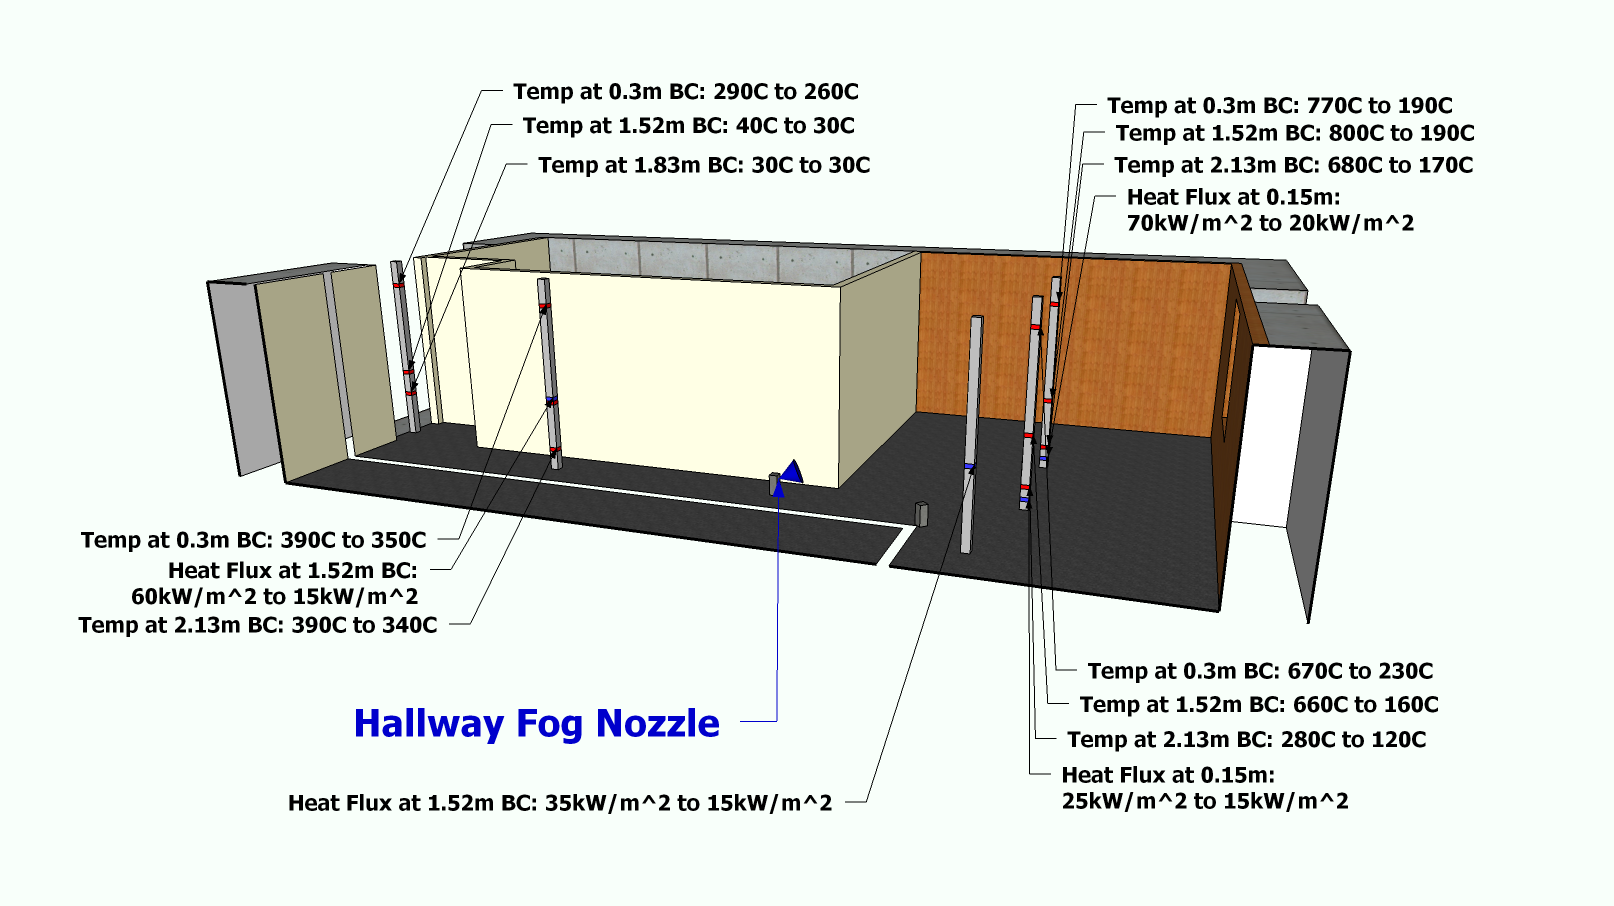
\includegraphics[width=\columnwidth]{../Figures/Pictures/Metric/DelCoFogTest1FirstSuppression}
	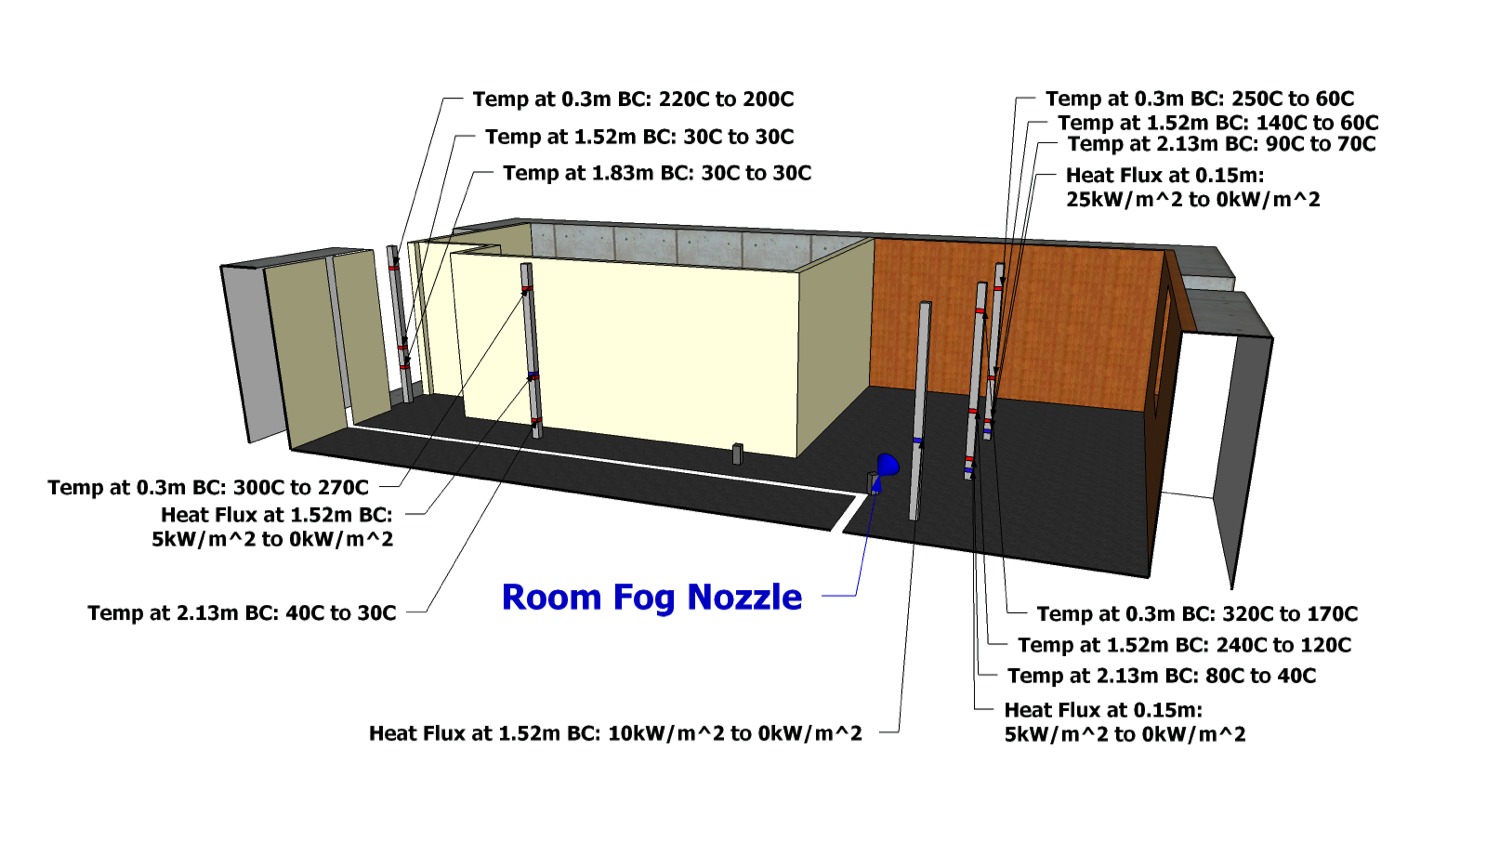
\includegraphics[width=\columnwidth]{../Figures/Pictures/Metric/DelCoFogTest1SecondSuppression}
	\caption{Impact of fire suppression actions on thermocouple and heat flux measurements for CAFS Test 1. The top image shows the hallway suppression impact and the bottom images shows the room suppression impact.}
	\label{fig:fs_1_1}
\end{figure}

Note that while there are some differences in the changes in temperature and heat flux when comparing CAFS to Water, differences are not substantial. Both suppression agents had similar, significant impact in reducing the high-temperature, high-heat flux environment that existed before suppression. The first (hallway) suppression, an indirect attack, did a majority of the cooling in all of the tests. This illustrates the impact of gas cooling, independent of suppression agent. In several cases rekindling occurred, as seen by the temperature increase between the two nozzle applications, but all cases the second (room) attack controlled the fire.

\subsubsection*{Two Story Structure}
\label{sec:fire_supp_two}

There were 7 suppression tests conducted in the two story purpose-built structure. All seven of the tests used a fuel load consisting of three sofas, polypropylene carpeting over polyurethane foam padding, and OSB paneling along three walls and the ceiling, and five of the seven tests had two stacks of wooden pallets in addition to this fuel load (Section~\ref{sec:fire_suppression_furniture_fuel}). Ignition occurred in the southwest corner of the basement and available ventilation was through the basement double doors and the 1st floor south door. The fires were intended to replicate room and contents basement fires typically seen within residential structures. Suppression occurred at the basement double doors of the structure. Table~\ref{tab:Test_Descriptions_2} provides an overview of the suppression tests conducted.

\begin{table}[!ht]
\centering
\footnotesize
\caption{Fire Suppression Test Descriptions}\label{tab:Test_Descriptions_2}
\begin{tabular}{clllll}
\toprule[1.5pt]
Test $\#$  & Name	& Stream			& Flow Rate		& Fuel                    & Ventilation  \\
\midrule
 38  & CAFS~7    &  Straight Stream  	&  120~gpm/60~cfm   & Furniture           & Basement Double Doors, 1st Floor Door \\
 39  & Water~7   &  Straight Stream  	&  120~gpm    		& Furniture           & Basement Double Doors, 1st Floor Door \\
 40a & CAFS~8a   &  Straight Stream  	&  120~gpm/60~cfm   & Furniture + Pallet  & Basement Double Doors, 1st Floor Door \\
 40b & CAFS~8b   &  Straight Stream  	&  120~gpm/60~cfm   & Furniture + Pallet  & Basement Double Doors, 1st Floor Door \\
 41a & Class A~1 &  Straight Stream  	&  120~gpm		    & Furniture + Pallet  & Basement Double Doors, 1st Floor Door \\
 41b & CAFS~9    &  1 3/8'' Ball    	&  120~gpm		    & Furniture + Pallet  & Basement Double Doors, 1st Floor Door \\
 41c & CAFS~9b   &  7/8'' Slub      	&  120~gpm		    & Furniture + Pallet  & Basement Double Doors, 1st Floor Door \\
\bottomrule[1.25pt]
\end{tabular}\par
\end{table}

Table~\ref{tab:Test_Results_2} provides the impact of suppression for the water and CAFS tests conducted in the two story structure. The measurement location is on the floor above the fire, at the doorway to the stairwell which connects the floor. This remote measurement location provides that is isolated from any direct contact from the suppression stream. The table provides change in temperature 0.3~m (1~ft) below the ceiling and 0.3~m (1~ft) above the floor as well as change in heat flux 1~m (3~ft) above the floor on the 1st floor level in front of the stairway door. The values reported in the table are immediately before and after the application period to assess the application agent, stream, and location on interior conditions.

\begin{table}[!ht]
\centering
\caption{Fire Suppression Results}\label{tab:Test_Results_2}
\begin{tabular}{lccc}
\toprule[1.5pt]
                     & \multicolumn{2}{c}{Temperature Change}                                    & Heat Flux Change \\
Test 	             & 0.3~m (1~ft) Below Ceiling          & 0.3~m (1~ft) Above Floor	         & 1~m (3~ft) Above Floor \\
\midrule
CAFS~7 Stairell      & 580~$^{\circ}$C - 260~$^{\circ}$C   & 490~$^{\circ}$C - 195~$^{\circ}$C   & 24~kW/m$^2$ - 17~kW/m$^2$  \\[.25cm]
Water~7 Stairwell    & 515~$^{\circ}$C - 260~$^{\circ}$C   & 455~$^{\circ}$C - 215~$^{\circ}$C   & 17~kW/m$^2$ - 17~kW/m$^2$  \\[.25cm]
CAFS~8a Stairwell    & 475~$^{\circ}$C - 285~$^{\circ}$C   & 425~$^{\circ}$C - 250~$^{\circ}$C   & 21~kW/m$^2$ - 14~kW/m$^2$  \\
CAFS~8b Stairwell    & 450~$^{\circ}$C - 240~$^{\circ}$C   & 390~$^{\circ}$C - 190~$^{\circ}$C   & 13~kW/m$^2$ - 12~kW/m$^2$  \\[.25cm]
Class A~1 Stairwell  & 440~$^{\circ}$C - 305~$^{\circ}$C   & 260~$^{\circ}$C - 235~$^{\circ}$C   & 13~kW/m$^2$ - 11~kW/m$^2$  \\
CAFS~9a Stairwell    & 470~$^{\circ}$C - 270~$^{\circ}$C   & 420~$^{\circ}$C - 235~$^{\circ}$C   & 17~kW/m$^2$ - 16~kW/m$^2$  \\
CAFS~9b Stairwell    & 510~$^{\circ}$C - 340~$^{\circ}$C   & 415~$^{\circ}$C - 295~$^{\circ}$C   & 20~kW/m$^2$ - 17~kW/m$^2$  \\
\bottomrule[1.25pt]
\end{tabular}\par
\end{table}

Similar to the single story fire suppression tests, there are some differences in the changes in temperature and heat flux when comparing CAFS to Water, but the differences are not substantial. Both suppression agents had similar, significant impact in reducing the high-temperature, high-heat flux environment that existed before suppression. 

\chapter{Discussion}
\label{chap:Discussion}

This study focused on two key types of fire experiments; gas cooling and fire suppression. In each type of experiment a comparison was conducted between plain water and compressed air foam being discharged from nozzles of similar type with similar mass flow rates.  In both types of experiments there were no measurable differences between the use of plain water or compressed air foam. These results were not surprising to some of the workshop attendees.  However other workshop attendees, that use CAF very successfully in their fire departments, had additional questions. The research team worked to address those follow-up questions by conducting additional fire suppression experiments, one where only wood based fuels were used and another where a larger space with more ventilation was used.  This section will discuss the results and provide potential explanations to support them.

\section{Gas Cooling}
\label{sec:Gas_Cooling_discuss}
 
Water is the most widely used fire extinguishing agent because it is effective, environmentally friendly, nontoxic, inexpensive and in many cases, readily available. In addition, water has a very high heat of vaporization per unit mass, at least four times as high as that of any other nonflammable liquid~\cite{NFPA}. The latent heat of vaporization of water is 2255~kJ/kg (970~Btu/lb.)~\cite{NFPA}. This means that 2255~kJ (2139~Btu) of energy is required to change 1~kg (2.2~lb.) of water into steam.  When water is vaporized, its volume increases approximately 1,700 times. Because the energy absorbing capabilities of water are well quantified, they can be used as a basis to calculate the theoretical minimum delivery rate of water needed to extinguish a burning material with a known heat (energy) release rate. Unfortunately, experience has shown that water must be applied at 10 to 100 times the theoretical rate in practice to control and extinguish the fire~\cite{Friedman:2}. As a result of this apparent inefficiency and the need to address fires containing a wide variety of materials, water-based fire fighting additives have been utilized for many years to enhance the fire fighting capabilities of ordinary water.

The most widely used of the water-based agents are the foams used on Class B (liquid hydrocarbon) fires. Agents designed primarily for Class A (ordinary combustible) fires have been used most extensively in conjunction with wildland fires. More recently these agents have been promoted for use on a wider range of Class A and in some cases Class B and D (combustible metal) fires. These agents are frequently claimed to be more effective than plain water while being environmentally safe. In some cases, they are also claimed to reduce the quantity and toxicity of smoke. To gain an understanding of how additives might enhance the fire suppression capabilities of water, it is important to examine the principles of fire suppression.

The gas cooling experiments were designed to measure the ability of water streams and CAFS streams to cool a hot gas layer with a minimum temperature of  250~$^{\circ}$C (482~$^{\circ}$F) at positions 1.83~m (6~ft) below the ceiling. During the planning of the experiments, some firefighters thought that the excellent heat absorbing capacity of plain water would exceed the heat absorbing capabilities of CAFS, since the injected air, air being a great insulator, would interfere and result in less cooling. It was the belief that the reduced gas cooling capabilities of CAFS may have lead to firefighter injuries during interior fire attacks. Other firefighters thought that the bubble structure would provide the same mass flowrate of water with more surface area, which would enable a faster heat transfer rate and therefore, improve the cooling of the hot gas layer. There were also thoughts that the CAFS would coat the ceiling and eliminate energy feedback from the ceiling to the hot gas layer, thereby providing enhanced cooling.

In each gas cooling experiment, the same mass flow rate of water was used for both the plain water stream and the CAF stream. Typically the volumetric flow rate of water was 7.57~L/s (120~gpm). The density of water is 1000~kg/m$^3$ (8.3~lb/gal), therefore the mass flow rate was 7.57~kg/s (16.7~lb/s).  The average time of flow was 15~s, therefore a total of 114~kg (251~lb) of water was introduced into each gas cooling experiment. When a CAFS stream was used it contained 0.3\% foam concentration by volume, check density of foam concentrate   point being mostly water.  Also calc the mass of air in the stream.

Compare flow rate with coverage estimates Iowa/NFA formulas. 

Ref Sean Mitchell report and then close with the ref back to the two comparison graphs.   Under the conditions of a residential scale room and contents fire it should be no surprise that the results are similar, the mass of water introduced into the hot gas layer is doing the work.  Air filled bubbles in the CAFS stream had no discernible impact in these experiments.   

\section{Fire Suppression}
\label{sec:Fire_Suppression_discussion}


\chapter{Summary}
\label{chap:Summary}

\chapter{Acknowledgments}
\label{chap:acknowledgments}

The authors would like to thank Roy McLane (currently with Thermal Fabrication), Kristopher Overholt (currently with Continuum Analytics), Keith Stakes (currently with UL FSRI), Adam Barowy (currently with UL), Kelly Opert (currently with UL) and Jay McElroy (retired) from NIST for their contributions in preparing and conducting these experiments. These experiments could not have been conducted without them. 

The Delaware County Emergency Services Training Center provided the location and logistical support for these experiments. The Delaware County team was under the direction of Kerby Kerber.

Thank you for assisting NIST in generating data that will assist the fire service in making tactical choices.


\bibliography{../../../Bibliography/FDS_refs,../../../Bibliography/FDS_general}

\appendix

\chapter{Spray Density Figures}
\label{app:spray_density}

\begin{figure}[ht]
\begin{tabular*}{\textwidth}{lr}
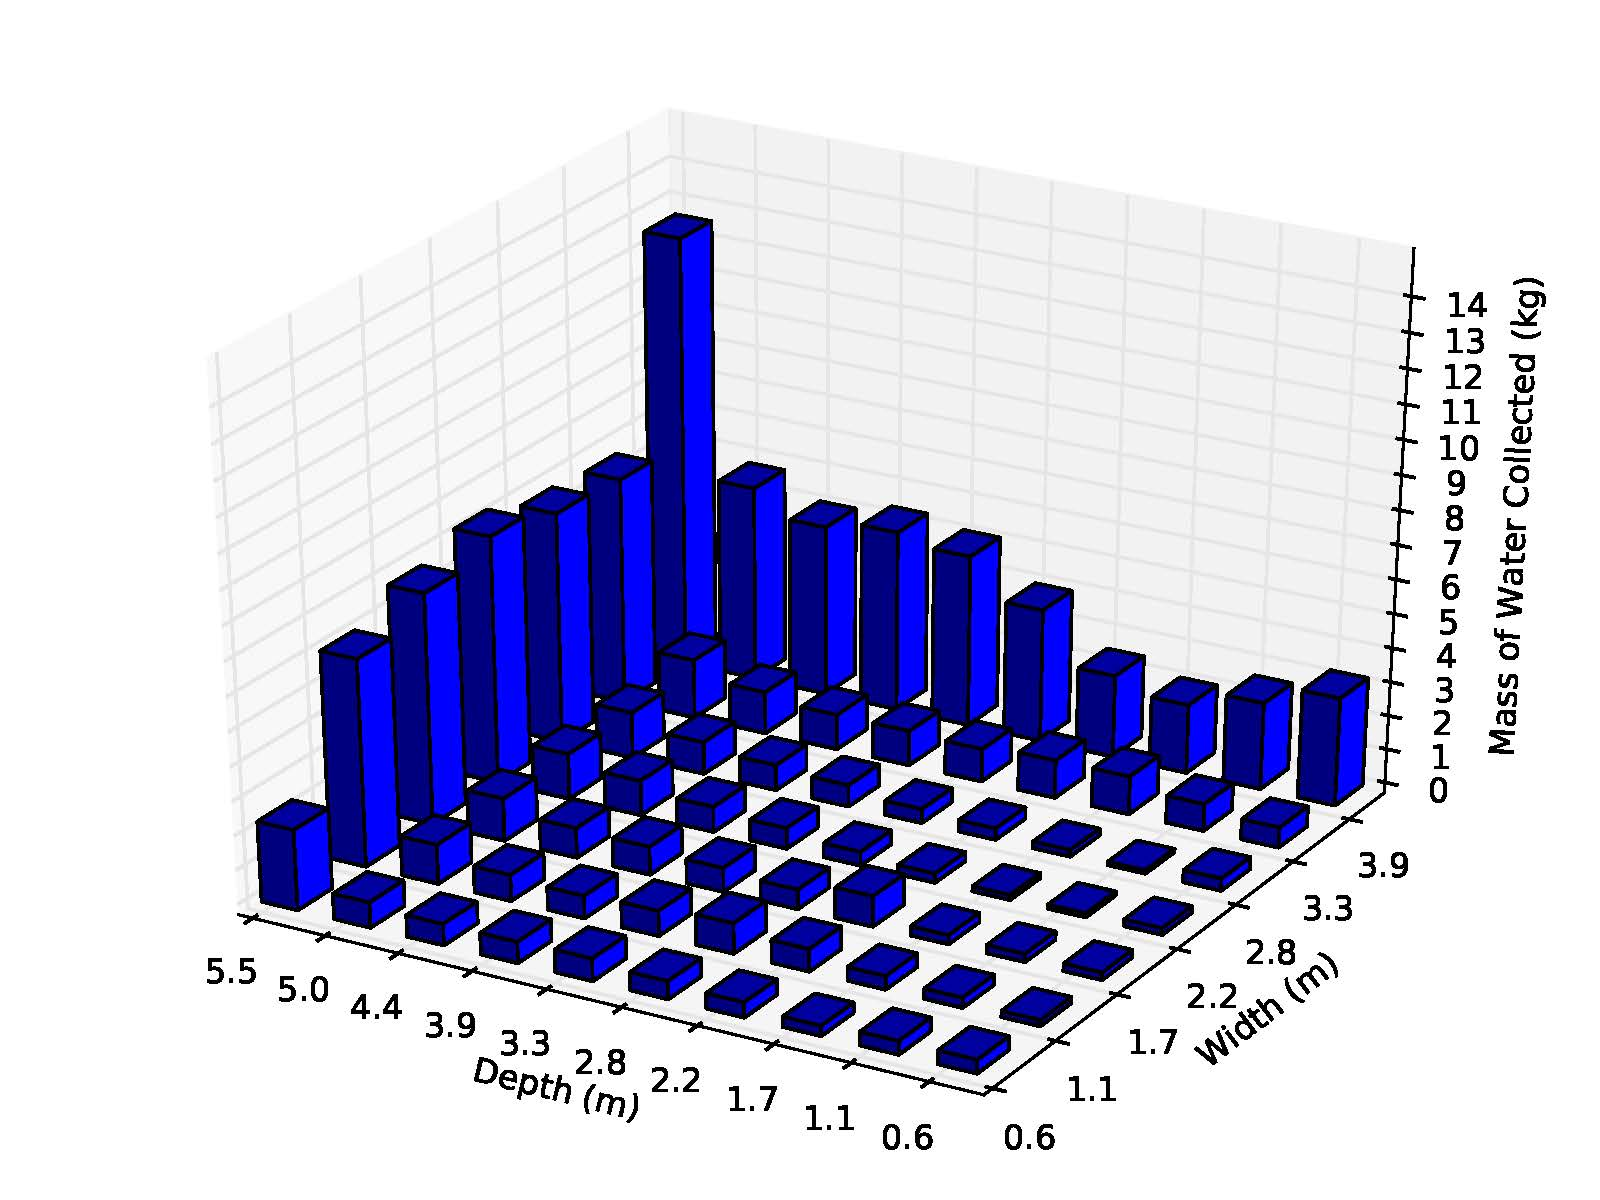
\includegraphics[width=3.2in]{../Figures/Bars/BB1} &
\includegraphics[width=3.2in]{../Figures/Bars/BB2} \\
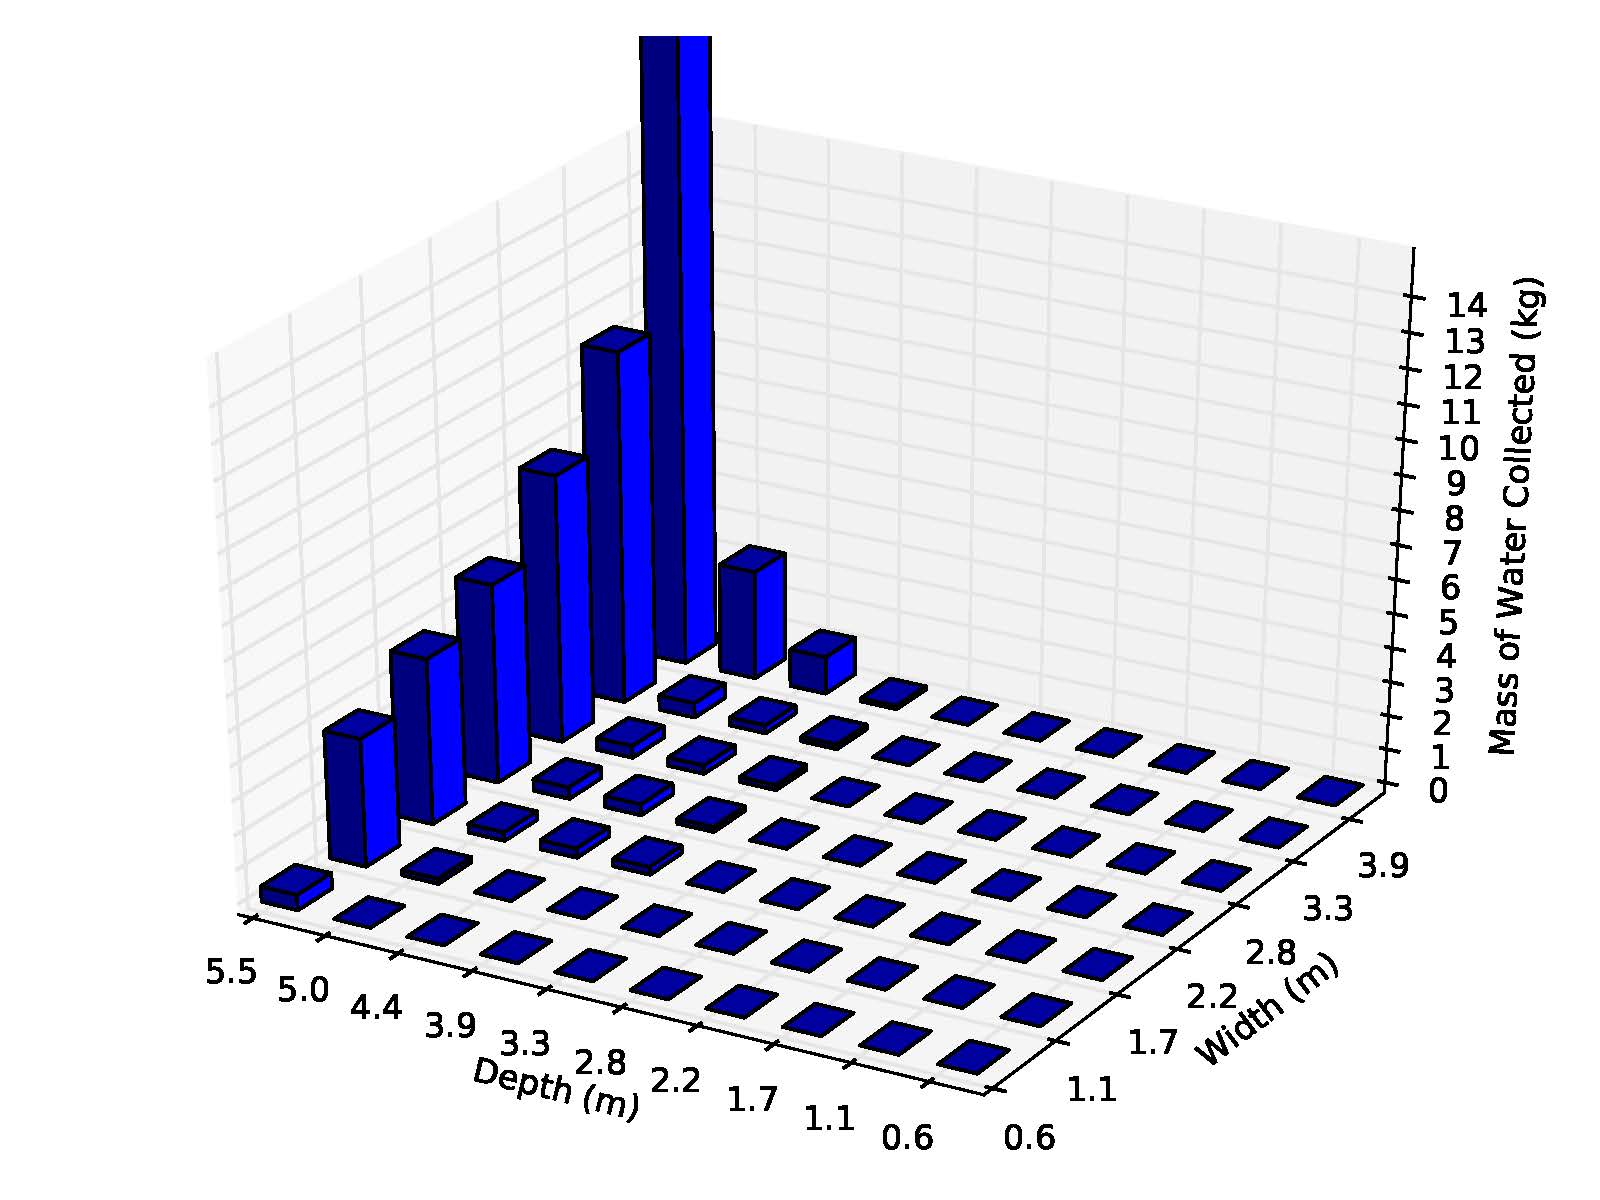
\includegraphics[width=3.2in]{../Figures/Bars/BB3} &
\includegraphics[width=3.2in]{../Figures/Bars/BB4}
\end{tabular*}
\caption{Spray density figures for burn building tests 1 (upper left), 2 (upper right), 3 (lower left), and 4 (lower right).}
\label{fig:bb_1_4}
\end{figure}

\clearpage

\begin{figure}[ht]
\begin{tabular*}{\textwidth}{lr}
\includegraphics[width=3.2in]{../Figures/Bars/BB5} &
\includegraphics[width=3.2in]{../Figures/Bars/BB6} \\
\includegraphics[width=3.2in]{../Figures/Bars/BB7} &
\includegraphics[width=3.2in]{../Figures/Bars/BB8}
\end{tabular*}
\caption{Spray density figures for burn building tests 5 (upper left), 6 (upper right), 7 (lower left), and 8 (lower right).}
\label{fig:bb_5_8}
\end{figure}

\clearpage

\begin{figure}[ht]
\begin{tabular*}{\textwidth}{lr}
\includegraphics[width=3.2in]{../Figures/Bars/BB9} &
\includegraphics[width=3.2in]{../Figures/Bars/BB10} \\
\includegraphics[width=3.2in]{../Figures/Bars/BB11} &
\includegraphics[width=3.2in]{../Figures/Bars/BB12}
\end{tabular*}
\caption{Spray density figures for burn building tests 9 (upper left), 10 (upper right), 11 (lower left), and 12 (lower right).}
\label{fig:bb_9_12}
\end{figure}

\clearpage

\begin{figure}[ht]
\begin{tabular*}{\textwidth}{lr}
\includegraphics[width=3.2in]{../Figures/Bars/BB13} &
\includegraphics[width=3.2in]{../Figures/Bars/BB14} \\
\includegraphics[width=3.2in]{../Figures/Bars/BB15} &
\includegraphics[width=3.2in]{../Figures/Bars/BB16}
\end{tabular*}
\caption{Spray density figures for burn building tests 13 (upper left), 14 (upper right), 15 (lower left), and 16 (lower right).}
\label{fig:bb_13_16}
\end{figure}

\clearpage

\begin{figure}[ht]
\begin{tabular*}{\textwidth}{lr}
\includegraphics[width=3.2in]{../Figures/Bars/BB17} &
\includegraphics[width=3.2in]{../Figures/Bars/BB18} \\
\includegraphics[width=3.2in]{../Figures/Bars/BB19} &
\includegraphics[width=3.2in]{../Figures/Bars/BB20}
\end{tabular*}
\caption{Spray density figures for burn building tests 17 (upper left), 18 (upper right), 19 (lower left), and 20 (lower right).}
\label{fig:bb_19_21}
\end{figure}

\clearpage

\begin{figure}[ht]
\centering
\includegraphics[width=3.2in]{../Figures/Bars/BB21}
\caption{Spray density figures for burn building test 21.}
\label{fig:bb_21}
\end{figure}

\clearpage

\begin{figure}[ht]
\begin{tabular*}{\textwidth}{lr}
\includegraphics[width=3.2in]{../Figures/Bars/ES_1} &
\includegraphics[width=3.2in]{../Figures/Bars/ES_2} \\
\includegraphics[width=3.2in]{../Figures/Bars/ES_3} &
\includegraphics[width=3.2in]{../Figures/Bars/ES_4}
\end{tabular*}
\caption{Spray density figures for experimental structure tests 1 (upper left), 2 (upper right), 3 (lower left), and 4 (lower right).}
\label{fig:es_1_4}
\end{figure}

\clearpage

\begin{figure}[ht]
\begin{tabular*}{\textwidth}{lr}
\includegraphics[width=3.2in]{../Figures/Bars/ES_5} &
\includegraphics[width=3.2in]{../Figures/Bars/ES_6} \\
\includegraphics[width=3.2in]{../Figures/Bars/ES_7} &
\includegraphics[width=3.2in]{../Figures/Bars/ES_72}
\end{tabular*}
\caption{Spray density figures for experimental structure tests 5 (upper left), 6 (upper right), 7 (lower left), and 7.2 (lower right).}
\label{fig:es_5_72}
\end{figure}

\clearpage

\begin{figure}[ht]
\begin{tabular*}{\textwidth}{lr}
\includegraphics[width=3.2in]{../Figures/Bars/ES_8} &
\includegraphics[width=3.2in]{../Figures/Bars/ES_9} \\
\includegraphics[width=3.2in]{../Figures/Bars/ES_10} &
\includegraphics[width=3.2in]{../Figures/Bars/ES_11}
\end{tabular*}
\caption{Spray density figures for experimental structure tests 8 (upper left), 9 (upper right), 10 (lower left), and 11 (lower right).}
\label{fig:es_8_11}
\end{figure}

\chapter{Fire Suppression Figures}
\label{app:fire_suppression}

\begin{figure}[ht!]
	\includegraphics[width=\columnwidth]{../Figures/Pictures/Metric/DelCoFogTest1FirstSuppression}
	\includegraphics[width=\columnwidth]{../Figures/Pictures/Metric/DelCoFogTest1SecondSuppression}
	\caption{Impact of fire suppression actions on thermocouple and heat flux measurements for CAFS Test 1. The top image shows the hallway suppression impact and the bottom images shows the room suppression impact.}
	\label{fig:app_fs_1}
\end{figure}

\begin{figure}[ht!]
	\includegraphics[width=\columnwidth]{../Figures/Pictures/Metric/DelCoFogTest2FirstSuppression}
	\includegraphics[width=\columnwidth]{../Figures/Pictures/Metric/DelCoFogTest2SecondSuppression}
	\caption{Impact of fire suppression actions on thermocouple and heat flux measurements for Water Test 1. The top image shows the hallway suppression impact and the bottom images shows the room suppression impact.}
	\label{fig:app_fs_2}
\end{figure}


\end{document}

